\documentclass[bibtotoc, liststotoc, BCOR5mm, DIV12, parskip=half+, pagesize=auto, twoside=false]{scrbook}

% use this declaration to set specific page margins
%\usepackage[a4paper , lmargin = {2.7cm} , rmargin = {2.9cm} , tmargin = {2.7cm} , bmargin = {4.6cm} ]{geometry}
\usepackage[a4paper]{geometry}

\usepackage[ngerman, english]{babel}
\usepackage[utf8]{inputenc}
\usepackage[numbers]{natbib}
\usepackage[default]{lato}
\usepackage[T1]{fontenc}
% \usepackage[latin1]{inputenc} % german characters
\usepackage{graphicx} 				% it's recommended to use PDF images but you can use JPG or PNG as well
\usepackage{url}           		% format URLs
\usepackage{hyperref} 				% create hyperlinks
\usepackage{listings, color}	% for source code
\usepackage{subfig}						% two figures next to each other (example: figure 3a), figure 3b)
\usepackage{scrpage2}					% header and footer line
\usepackage{csquotes}
\usepackage{amsmath}
\usepackage{sidecap}
\usepackage{tikz}
\usepackage{pgfplots}
\usepackage{minted}
\usepackage{mdframed}
\usepackage{booktabs}
\usepackage{pdfpages}
% \usepackage[default,scale=0.95]{opensans}
% \usepackage[final]{microtype} % mikrotypographische Optimierungen

%tables
\usepackage{multirow} % Tabellen-Zellen über mehrere Zeilen
\usepackage{multicol} % mehre Spalten auf eine Seite
\usepackage{tabularx} % Für Tabellen mit vorgegeben Größen
\usepackage{longtable} % Tabellen über mehrere Seiten
\usepackage{float}

\usepackage{setspace} % Zeilenabstand
% \onehalfspacing % 1,5 Zeilen
\linespread{1.1}
\usetikzlibrary{decorations.pathreplacing, arrows,matrix,positioning, fit, arrows.meta, chains}
% \usepackage{minted}
% header and footer line - no header & footer line on pages where a new chapter starts
\pagestyle{scrheadings}
\ohead{}
\ihead{}
% \ofoot[]{\thepage}
% \ifoot{Diploma Thesis, TU Berlin, Fachgebiet AV, 2009}

% set path where images are stored
\graphicspath{{./img/}}

%
% der Befehl \hypenation versteht keine Sonderzeichen, also weder �
% noch "a noch \"a. W�rter die derartige Zeichen enthalten m�ssen
% direkt im Text getrennt werden, z.B. W�r\-ter
%
\hyphenation{te-le-com-muni-cation 
te-le-com-muni-cation-specific 
Te-le-kom-mu-ni-ka-tions-API} 					% use this file to set explicit hyphenations (doesn't seem to work correctly)

\setlength{\parindent}{0pt}

\begin{document}
% ---------------------------------------------------------------
\frontmatter
    \thispagestyle{empty}
\begin{center}

\vspace*{0.3cm}
{\LARGE \textbf{Technische Universit{\"a}t Berlin}}

\vspace{0.3cm}

{\large Institut f{\"u} Softwaretechnik und Theoretische Informatik\\[1mm]}
{\large Quality and Usability Lab\\[5mm]}

Fakultaet IV\\
Franklinstrasse 28-29\\
10587 Berlin\\

\vspace*{1cm}


\includegraphics[width=4cm]{tu_logo.jpg}

\vspace*{1.0cm}

{\LARGE Master Thesis}\\
\vspace{0.3cm}
{\large M.Sc. Computer Science}\\

\vspace{0.8cm}
{\LARGE \textbf{Predicting tap locations on touch screens in the field using accelerometer and gyroscope sensor readings}}\\
\vspace*{0.8cm}
{\LARGE Emanuel Schmitt}
\\
\vspace*{0.5cm}
Matriculation Number: 333772\\
\vspace*{1.0cm}

Examined by:\\
Prof. Dr.-Ing. Sebastian M{\"o}ller\\
Prof. Dr.-Ing. Axel Ku{\"u}per\\
\vspace*{0.3cm}
Supervised by:\\
Dr.-Ing. Jan-Niklas Antons\\
Carola Trahms
\vspace{3cm}


\end{center}


   	\thispagestyle{empty}
    \cleardoublepage
    
    \thispagestyle{empty}
\vspace*{3cm}

Thanks to all dem brothas
    \thispagestyle{empty}
    \cleardoublepage
    
    \newpage

\thispagestyle{empty}

\begin{large}

\vspace*{6cm}

\noindent
Hereby I declare that I wrote this thesis myself with the help of no more than the mentioned literature and auxiliary means.
\vspace{2cm}

\noindent
Berlin, 15.10.2017

\vspace{3cm}

\hspace*{7cm}%
\dotfill\\
\hspace*{8.5cm}%
\textit{(Signature [your name])}

\end{large}
 
    \thispagestyle{empty}
    \cleardoublepage
    
    
    \thispagestyle{empty}
\vspace*{1.2cm}

\begin{center}
    \textbf{Abstract}
\end{center}

\vspace*{0.5cm}

\noindent

Recent research has shown that the location of touch screen taps on modern smartphones and tablet computers can be identified based on sensor recordings from the device's accelerometer and gyroscope. This security threat implies that an attacker could launch a background process on the mobile device and send the motion sensor readings to a third party vendor for further analysis. Even though the location inference is a non-trivial task requiring machine learning algorithms in order to predict the tap location, previous research has shown that PINs and passwords of users could be successfully obtained. However, as the tap location inference was only shown for taps generated in a controlled setting not reflecting the environment users naturally engage with their smartphones, the attempts in this work bridge this gap.

In this work, I propose TapSensing, a data acquisition system designed to collect touch screen tap event information with corresponding accelerometer and gyroscope readings. Having performed a data acquisition study with 27 subjects and 3 different iPhone models, a total of 45,000 labeled taps could be acquired from a laboratory and field environment enabling a direct comparison of both. The overall findings show that tap location inference is generally possible for data acquired in the field, hence, with a performance reduction of approximately 20\% when comparing both environments. As the tap inference has therefore been shown for a more realistic data set, this work yet again confirms that smartphone motion sensors could potentially be used to comprise the user's privacy.
    \thispagestyle{empty}
    \cleardoublepage
    
    \thispagestyle{empty}
\vspace*{1.2cm}

\begin{center}
    \textbf{Zusammenfassung}
\end{center}

\vspace*{0.5cm}

\noindent

Untersuchungen haben gezeigt, das die Position eines Taps auf einem Smartphone oder Tablet Displays \"uber eine Aufzeichnung der Lagesensoren bestimmt werden kann. Diese Sicherheitsl\"ucke deutet darauf hin, dass ein potentieller Angreifer einen Hintergrundprozess auf dem Zielger\"at installieren und die aufgezeichneten Daten an eine Server Applikation zur weiteren Analyse schicken k\"onnte. Obwohl die Bestimmung der Postion auf dem Touchscreen keine einfache Aufgabe darstellt, die nur mit Hilfe von Maschi-nellem Lernen m\"oglich ist, ist es Forschern dennoch gelungen PINs und Passw\"orter von einzelnen Nutzern auszusp\"ahen. Da jedoch die Daten zur Vorhersage in den bisherigen Versuchen von Nutzern stammen, die in einem Laborversuch aufgezeichnet wurden und die Daten hierbei keine reale Nutzerumgebung darstellen, schliesst diese Arbeit diese L\"ucke.

In dieser Arbeit stelle ich TapSensing vor, eine Applikation die Touch Screen Interaktionen mit den entsprechenden Lagesensor-Daten aufzeichnet. In einem Labor sowie in einem Feldversuch mit insgesamt 27 Teilnehmer, wurden 45.000 einzelne Taps aufgenommen. In einer Analyse konnte gezeigt werden, dass eine Vorhersage der Tap-Position auf dem Display ebenso f\"ur Daten aus dem Feld m\"oglich ist. Im direkten Vergleich zwischen Feld und Labor wurden jedoch Performance-Einbußen von rund 20\% f\"ur Daten aus dem Feld gemessen. Da die Tap-Positions-Inferenz nun f\"ur reale Konditionen gezeigt werden konnte, k\"onnen wir uns bisherigen Untersuchungen anschließen und erneut bestätigen, dass Lagesensoren ein potentielles Sicherheitsrisiko f\"ur den Nutzer darstellen.
% Die Forschung hat gezeigt, dass der Standort von Touchscreen-H\"ahnen auf modernen Smartphones und Tablet-Computern basierend auf Sensoraufzeichnungen von Beschleunigungsmesser- und Gyroskop-Messwerten des Ger\"ats identifiziert werden kann. Diese Sicherheitsbedrohung impliziert, dass ein Angreifer einen Hintergrundprozess auf dem Mobilger\"at starten und die Bewegungssensordaten zur weiteren Analyse an einen Drittanbieter senden kann. Obwohl dies eine nicht triviale Aufgabe ist, die Algorithmen zum maschinellen Lernen erfordert, um den Abzweigort vorherzusagen, haben bisherige Untersuchungen gezeigt, dass PINs und Kennw\"orter von Benutzern erhalten werden k\"onnen. Da die Klopfort-Inferenz jedoch nur f\"ur Taps dargestellt wurde, die in einer kontrollierten Umgebung erzeugt wurden, die die Umgebung nicht widerspiegelt, die Benutzer von Natur aus mit ihren Smartphones besch\"aftigen, versucht diese Arbeit diese L\"ucke zu schließen.

% In dieser Arbeit empfehle ich TapSensing, ein Datenerfassungssystem, das Touchscreen-Tap-Event-Informationen mit entsprechenden Beschleunigungsmessern und Gyroskop-Messwerten erfasst. Mit einer Datenakquisitionsstudie mit 27 Probanden und 3 verschiedenen iPhone-Modellen konnten insgesamt 45.000 markierte Abgriffe aus einer Labor- und Feldumgebung gewonnen werden, die einen Vergleich erm\"oglichen. Die Gesamtergebnisse zeigen, dass eine Klopfortinferenz generell f\"ur im Feld erfasste Daten m\"oglich ist, jedoch mit einer Leistungsreduzierung von ungef\"ahr 20%, wenn beide Umgebungen verglichen werden. Da die Tipping-Inferenz daher f\"ur einen realistischeren Datensatz gezeigt wurde, und indem sie sich an die vorherigen Experimente anlehnt, best\"atigt diese Arbeit erneut, dass Smartphone-Bewegungssensoren potentiell verwendet werden k\"onnen, um die Privatsph\"are des Benutzers zu umfassen.


\noindent 
    \thispagestyle{empty}
    
    
    \tableofcontents
   
    \thispagestyle{empty}
    
    \listoffigures
    \thispagestyle{empty}
    
    \listoftables
    \thispagestyle{empty}
    
% --------------------------------------------------------------

\mainmatter % comment single chapters for faster compilation

    \chapter{Introduction\label{cha:chapter1}}
The utilization of smartphones has become an integral part of our everyday life. We use them to perform various tasks ranging from highly privacy-sensitive tasks such as for bank transactions or personal communication to more casual tasks such as setting an alarm clock or checking the weather. This universal applicability is one important factor that has contributed to the immense success of the smartphone. Another factor is the rich set of embodies sensor, such as an accelerometer, digital compass, gyroscope, GPS, microphone and camera \cite{5560598} which have enabled developers to introduce highly interactive applications.
%  that provide valuable services to the ever growing smartphone user base.


% The utilization of smartphones has become an integral part of our everyday life. Smartphones are used for all sorts of tasks ranging from more privacy-sensitive tasks such as bank transactions or personal communication to more casual tasks such as setting an alarm clock or checking the weather. The success of the smartphone is partly due to it's rich set of embodied sensors, such as an accelerometer, digital compass, gyroscope, GPS, microphone and camera \cite{5560598}. These sensor have enabled developers to introduce highly interactive applications providing valuable services to the ever growing smartphone user base.

% Augumented reality ++
Location based services, for instance, utilizing the GPS sensor \cite{link2011footpath} can lead users on the fastest route to their desired destination while health tracking applications \cite{case2015accuracy}, enabled by the motion sensors, can recommend health beneficial behavior based on the amount of physical activity sensed. Furthermore, newly introduced augmented reality applications utilize the camera and the motion sensors to enhance our perception of our immediate surroundings resulting in a whole new interactive experience. As these are positive examples for sensor usage, there have also been reports of sensor utilization with a more malicious intent.

The motion sensors, gyroscope and accelerometer, which are typically used for detecting the device orientation and for gaming applications \cite{feijoo2012mobile}, can be used to infer the locations of touch-screen taps. As the striking force of a tapping finger creates an identifiable signature on the 3-axis motion sensors, previous research has shown that the granularity of inference is adequate to obtain PINs and passwords \cite{Touchlogger, Tapprints, Accessory} or at least significantly reduce the search space to do so. The situation is furthermore reinforced by the fact that motion sensors do not require special privileges or access rights on operation system level. Due to this purpose, the motion sensors expose a vulnerable side-channel for potential attackers to eavesdrop on user interactions.

However, as the motion data used to train the inference systems in the previous research was acquired from users in a controlled setting \cite{Tapprints, Touchlogger, Accessory}, the feasibility of tap location inference has not been shown for a more realistic data set that is capable of modeling natural user behavior as well as their changing environments. It is plausible that when a user interacts with the touch screen, for instance, while walking in the park or during a public transportation ride, the sensory data will be effected by this activity potentially mitigating an eavesdropping attack.

In order to address this issue, I would like to propose \textit{TapSensing}. TapSensing is a data acquisition system designed to acquire tap information with corresponding accelerometer and gyroscope readings. After having conducted a laboratory and field study, I have collected over 45,000 taps from 27 different subjects to investigate if the proposed security threat posed by leaking motion sensor also applies to an uncontrolled environment.

% Similar to the previous data acquisition systems, \textit{TapSensing} is capable of collecting tap event information with corresponding accelerometer and gyroscope readings. In this thesis, \textit{TapSensing} was used to collect tap data in a laboratory as well as a field study in order to 
% %---here!!
% In order to investigate this issue, I propose \textit{TapSensing}. TapSensing is 
% In order to find out if tap inference is possible in the field, two , I would like to propose \textit{TapSensing}. \textit{TapSensing} is an iOS application designed to acquire tap data with corresponding gyroscope and accelerometer recordings. In a user study with 27 participants, I have collected over 45.000 taps acquired from the laboratory as well as the field environment in order to compare the feasibility of touch-screen tap inference for both environments.

\section{Motivation}

In recent years, the number of smartphone users has rapidly
increased. According to a report published by Smart
Insights\footnote{http://www.smartinsights.com/mobile-marketing/mobile-marketing-analytics/mobile-marketing-statistics/}, the number of smartphone users grew from 400 million users in 2007, to more than 1,800 million in 2015. In addition, the report claims that at the end of 2017, 97\% of adults, aged 18 to 34, in the US were mobile device users. Due to this rapid adaption and the smartphones rich set of sensors, smartphones have increasingly become targets for various attacks \cite{Colp:2015:PDS:2694344.2694380, Aviv:2010:SAS:1925004.1925009, Touchlogger}.

As gyroscope and accelerometer are commonly used for all genres of applications ranging from gaming \cite{feijoo2012mobile} to productivity apps \cite{pylvanainen2005accelerometer}, the mobile operating system providers offer easy-to-use access via standard APIs\footnote{Application Programming Interface}. Consequently, a smartphone application designed for a real-world attack could sense the user's motion in the background and send the information to a server-side application for machine learning analysis. This is possible due to the fact that background tasks are fully supported on the Android platform while on iOS, methods have been developed to run initially prohibited background tasks\footnote{https://github.com/yarodevuci/backgroundTask} for long durations than usually supported. Notably, all this can be achieved without the user's consent due to the lack of access restriction for motion sensors.

A further point emphasizing the security threat is that in 2017 the World Wide Web Consortium, W3C, has released the so-called Device Orientation specification \cite{w3c} for JavaScript. This specification allows browser applications to access the motion sensor hardware of smartphones opening further possibilities for an attacker. A potentially harmless website could therefore obtain the motion sensor data and reveal private information of the user.

% As the data used for training the inference systems in previous research concerning the topic at hand was collected in a laboratory environment, it is assumed that the data collected in a field environment will be 

Besides all the privacy issues motion sensors raise, tap location inference could also be used for usability research purposes. Assuming that the inference provides high enough accuracies, it could be used as an in-app behavior tracking for applications where the source code is publicly not available. The inference system could run in a background task to evaluate the user behavior in a target application.

\section{Outline}
This work is structured as follows:

\begin{itemize}
  \item \textbf{Related Work}: In chapter 2, previous research concerning side-channel attacks is presented. As this work is based on similar studies, they will be outlined in this chapter.
  \item \textbf{Machine Learning Fundamentals}: In chapter 3, I will review the machine learning fundamentals required to understand the technical aspects of this thesis. Since learning the relation between the sensory data and the tap location is a supervised learning task, the classification algorithms used in this thesis will be introduced.
  \item \textbf{Data Aquisition System}: In chapter 4, I will introduce \textit{TapSensing} which is the data acquisition system used for obtaining taps and sensor readings for both the laboratory and the field environment.
  \item \textbf{Methodology}: In chapter 5, the methodology of the data acquisition, data pre-processing and machine learning classification is explained.
  \item \textbf{Results}: In chapter 6, meaningful results are presented from the data acquired in the user study.
  \item \textbf{Conclusion}: In the final chapter 7, I will conclude the thesis with an overview of the results and ideas for future studies.
\end{itemize}

% The rotation of the device is larger when the tap occurs
% at the edge of the device. The linear acceleration of the
% device may also be different, depending on how the finger
% pressure is absorbed by the phone’s metal/glass structure
% and casing. Of course, sensor noise and other factors will
% indeed pollute these signals, and in reality the problem of
% identifying a particular key-press from sensor data alone is
% hard. Nevertheless, theoretically, it should be conceivable
% that finger taps could have a fingerprint.



% Thus, when a user taps on different parts of the screen, it
% is entirely feasible that these taps produce an identifiable
% pattern on the 3-axis accelerometer and gyroscope.


% The motion of a smartphone during typing depends on
% several factors: 1) the striking force of the typing finger;
% 2) the resistance force of the supporting hand; 3) the
% landing location of the typing finger; and 4) the location
% of the supporting hand on the smartphone. The first two
% factors mainly affect the shift of the phone, while the latter
% two mainly affects the rotation. We observe that the
% first two factors likely depend on the user, while the latter
% two are likely to be user-independent because (1) on
% each soft keyboard configuration, each key is at a fixed
% location, and (2) a user typically holds her smartphone in
% a consistent way. Therefore, we would like to extract the
% rotation components while filtering out the shift components
% from motion sensor data



% Recent advances in data analytics have enabled a variety of new applications. 


% - Example applications GPS location based services, health tracking, zoom into behavioral patterns

% - Gyrscope and Accelerometer typicall used for detecing orientation or for gaming, VR 


% The utilization of smartphones has become an integral part of our everyday life. We use our smartphones throughout the day to to perform tasks such as casually checking the weather to more privacy sensitive tasks such as performing bank transactions or personal communication. The deployment of high resolution sensors embodied within these devices have enabled developers to build rich applications providing value services to it's ever growing customer base. Location based services, for instance, utilizing the GPS sensor can lead smartphone users on the fastest route to their desired destination. Furthermore, Health trackings applications can monitor the physical activity of users by tracking the user's motion and can thus recommend health beneficial behavior.



% The utlization of smartphones has become an integral part of our everyday life. Smartphones are used from checking the weather to more privacy sensitive tasks such as private communication or bank transactions. The deployment of high-resolution sensors within these devices and recent enhancements in data analytics have enabled a broad range of applications that provide valuable services to its users. Location based services, such as navigation devices, which utilize the GPS sensor can efficiently lead a user on the fastest route to his desired destination. 

% The utilization of smartphones has become an integral part of our everyday life. Smartphones are used as an alarm clock in the morning, as a communication devices during the day and even in some cases as a reading device before going to bed at night. Due to this habitual smartphone usage, we heavily interact with touchscreen throughout the day. \\

% The deployment of high-resolution sensors within these devices and recent enhancements in data analytics have enabled a broad range of applications that provide valuable services to its users. Location based services, such as navigation devices, which utilize the GPS sensor can efficiently lead a user on the fastest route to his desired destination. Health and fitness applications leveraging sensor readings from the accelerometer and gyroscope can track user specific patterns to recommend health improving behavior \cite{pushNot}. \\

% Previous research has shown that it is possible to predict tap locations on a touch screen by utilizing data collected from accelerometer and gyroscope sensor readings \cite{Touchlogger,Tapprints, acc}. However, since the previous work has been limited to using data from a laboratory environment, we would like to investigate if the predictability of tap locations is also applicable to a more realistic data sets. It is plausible that sensor data collected from subjects in the field can include noise making an inference less accurate. To examine these assumptions and to shed light into possible measures effecting these accuracies, we will conduct a laboratory as well as a field study in order to obtain the required data.

% - sensors in mobile smartphones
% - was kann man alles damit machen
% - wearables fitness tracker, gaming, GPS, navigation

% - high resolution sensors
% - handsets are everywhere
% - rapid growth
% - developers build highly interactive applications
% - privacy senstitive tasks are done on movile phones

% - security risks from cameras
% - combine sensors with data analistics - heart rate monitoring

% - previous research has shown that

% - Thus, when a user taps on different parts of the screen, it
% is entirely feasible that these taps produce an identifiable
% pattern on the 3-axis accelerometer and gyroscope. Figure
% 1 illustrates the intuition.

% Motivation 
% - javascript MDN

% sensor information from mobile devices – specifically from
% the accelerometer and gyroscope – can be adequate to infer
% the locations of touch-screen taps.


% Smartphones are ubiquitous. An ever-expanding consumer base
% carries their handsets everywhere. However, this rapid growth comes
% with new risks. While the proliferation of smartphones equipped
% with high-resolution sensors has afforded developers an opportunity
% to create highly interactive applications, users now rely on their smartphones
% to perform many privacy-sensitive tasks, such as online financial
% transactions and personal communications, that can be eavesdropped
% or exploited. In this paper, we argue that current security
% measures in mobile platforms do not adequately address the malware
% that exploits these high-resolution sensors.
% Current smartphone platforms allow developers access to certain
% hardware sensors (e.g., accelerometers) without requiring special privileges
% or explicit user consent. The security risks posed by microphones
% and cameras have been well documented [18, 21]. However,
% the security risks of accelerometers have so far been largely


% The proliferation of sensors on mobile devices, combined
% with advances in data analytics, has enabled new directions
% in personal computing. The ability to continuously sense
% people-centric data, and distill semantic insights from them,
% is a powerful tool driving a wide range of application domains.
% These domains range from remote patient monitoring,
% to localization, to fine grained context-awareness [16, 3,
% 2, 24]. While this ability to zoom into behavioral patterns
% and activities will only get richer over time, it is not surprising
% that there will be side effects. The research community
% and industry are already facing the ramifications of exposing
% location information; rumor has it that insurance companies
% are on the lookout to mine an individual’s dietary pattern to
% guide insurance cost and coverage. While these kind of side
% effects will continue to surface over time, this paper exposes
% one that may be particularly serious. Briefly, we find that
% sensor information from mobile devices – specifically from
% the accelerometer and gyroscope – can be adequate to infer
% the locations of touch-screen taps. Interpreted differently, a
% background process running on a mobile device may be able
% to silently monitor the accelerometer and gyroscope signals,
% and infer what the user is typing on the software keyboard.
% Needless to say, the ramifications can be monumental.
% This finding may not be surprising when one contemplates
% about it. Modern mobile devices, like smartphones
% and tablets, are being upgraded with sensitive motion sensors,
% mostly to support the rapidly growing gaming industry.
% Thus, when a user taps on different parts of the screen, it
% is entirely feasible that these taps produce an identifiable
% pattern on the 3-axis accelerometer and gyroscope. Figure
% 1 illustrates the intuition.

% We show that accelerometer readings are suffi-
% cient to extract sequences of entered text on smartphones. We create
% and evaluate a predictive model, trained only on acceleration
% measurements, of the security-sensitive task of password entry. We
% present findings on the inference accuracy as a function of the sampling
% frequency of the accelerometer, the on-screen location of the
% keypress, and the size of the predicted screen region. Additionally,
% we present measures for mitigating this side channel.


% This chapter should have about 4-8 pages and at least one image, describing your topic and your concept. Usually the introduction chapter is separated into subsections like 'motivation', 'objective', 'scope' and 'outline'.

% \section{Motivation\label{sec:moti}}

% Start describing the situation as it is today or as it has been during the last years. 'Over the last few years there has been a tendency... In recent years...'. The introduction should make people aware of the problem that you are trying to solve with your concept, respectively implementation. Don't start with 'In my thesis I will implement X'.

% \section{Objective\label{sec:objective}}

% \section{Outline\label{sec:outline}}

% The 'structure' or 'outline' section gives a brief introduction into the main chapters of your work. Write 2-5 lines about each chapter. Usually diploma thesis are separated into 6-8 main chapters. 
% \\
% \\
% \noindent This example thesis is separated into 7 chapters.
% \\
% \\
% \textbf{Chapter \ref{cha:chapter2}} is usually termed 'Related Work', 'State of the Art' or 'Fundamentals'. Here you will describe relevant technologies and standards related to your topic. What did other scientists propose regarding your topic? This chapter makes about 20-30 percent of the complete thesis.
% \\
% \\
% \textbf{Chapter \ref{cha:chapter3}} analyzes the requirements for your component. This chapter will have 5-10 pages.
% \\
% \\
% \textbf{Chapter \ref{cha:chapter4}} is usually termed 'Concept', 'Design' or 'Model'. Here you describe your approach, give a high-level description to the architectural structure and to the single components that your solution consists of. Use structured images and UML diagrams for explanation. This chapter will have a volume of 20-30 percent of your thesis.
% \\
% \\
% \textbf{Chapter \ref{cha:chapter5}} describes the implementation part of your work. Don't explain every code detail but emphasize important aspects of your implementation. This chapter will have a volume of 15-20 percent of your thesis.
% \\
% \\
% \textbf{Chapter \ref{cha:chapter6}} is usually termed 'Evaluation' or 'Validation'. How did you test it? In which environment? How does it scale? Measurements, tests, screenshots. This chapter will have a volume of 10-15 percent of your thesis.
% \\
% \\
% \textbf{Chapter \ref{cha:chapter7}} summarizes the thesis, describes the problems that occurred and gives an outlook about future work. Should have about 4-6 pages.
    \chapter{Related Work\label{cha:chapter2}}
The utilization of motion sensors sidechannels in order to reconstruct user interactions can be seen as a form of eavesdropping. Hence, in order to shed light into this category of security breaches, this chapter will cover past research based on the usage of side-channels emanations which can reveal confidential information. Therefore, The first section will cover different techniques that utilize acoustic, electromagnetic, optical and motion emanation for eavesdropping purposes while the second section shows related work aiming at inferring tap interactions on touchscreens.

\section{Eavesdropping on Emanations}

Eavesdropping is defined as the the practice of secretly listening to private conversations of others without their consent \cite{black1990black}. As this definition originally refers to conversations between humans, eavesdropping can also be seen in terms of human-computer-interaction. In this context, the computer is seen as one conversational partner whereas the user interacting with the device is seen as the other. As the channel of communication in a human conversation is the acoustic channel, the channel in which human-computer interaction takes place has various forms. Typically, a human may enter information on a peripheral device while the computer gives feedback through an image representation. However, speech interfaces and other forms of interaction are also possible. In order to spy on the human-computer conversation, a third party with malicious intent must apply different techniques in order to spy on these interactions.\\

In this context, a frequently discussed practice throughout academia involves the use of leaking emanations for eavesdropping purposes. These emanations can be monitored in order to carefully reconstruct the contained information. As these emanations occur in various formats, a categorization has been done based on the sensory channel they transpire. Therefore, the following sections will cover eavesdropping techniques based on acoustic, optical, electromagnetic and motion emanations.

% Eavesdropping is secretly listening to the private conversation of others without their consent, as defined by Black's Law Dictionary.[1]
% two words in interaction and 
% Inferring user interactions through side channels has been of great interest to the academic world throughout history. As this thesis will cover a modern approach by recording sensory information provided by the Apple iPhone, an early and prominent example of spying on emanations reaches far back in time. \\

%   % not having to modify the host system.

% Ever since, various user interaction inference experiments have been conducted by researchers worldwide. However, in order to categorize these different approaches found in literature, we will divide these based on the emanation channel that was spied on. This categorization approach is more suitable since device model and user interaction strategies have frequently changed in time.\\ 

% The literature denoted that user inference can be perused with the help of acoustic, optical, electro-magnetic and on sensory emanation. We will describe these in the following sections.

\subsection{Acoustic Emanations}
One way of spying on electrical devices is by utilizing the acoustic channel \cite{Backes:2010:ASA:1929820.1929847,1301311,Zhuang:2009:KAE:1609956.1609959}. Many electronic devices deploy tiny mechanics that generate sounds as a byproduct during interactions or during operation. These distinct sounds can differ in their characteristics making them adequate to identify the original information currently being processed by the machine. In these scenarios an eavesdropper targets a microphone in near proximity of the target device to capture the audio signals the device is exposing. A learning algorithm is then applied to the audio signals to reconstruct information. \\

In 2010, \citeauthor{Backes:2010:ASA:1929820.1929847} examined the problem of acoustic emanations of dot matrix printers, which where, at that time, still commonly used in banks and medical offices. By using a simple consumer-grade microphone, the researchers were able to recover whole sentences the printer was printing based. \citeauthor{Backes:2010:ASA:1929820.1929847} processed the audio samples in order to extracted frequency-domain features. These features worked as input for a hidden markov model, a technology commonly used in audio speech recognition. As a result, the recognition system was able to reconstruct individual characters based on the sound inputs. To demonstrate a potential attack, the researchers deployed the system in a medical office being able to obtain up to 72\% of the sentences being printed on medical subscriptions \cite{Backes:2010:ASA:1929820.1929847}. \\

Being inspired by the findings concerning the dot matrix printer, \citeauthor{1301311} investigated acoustic emanations produced by hitting keystrokes on a desktop and a notebook keyboard. Following their hypothesis claiming that each keystroke has a macroscopic difference in it's construction mechanics, as well as a distinct reverberation caused by the position in the board, individual keystrokes were recorded \cite{1301311}. Researchers then extracted frequency domain features from the audio signals and passed them into a neural network. In an experiment performing 300 keystrokes, 79\% of the characters could be correctly recognized \cite{1301311}. As this technique required substantial training before recognition, other studies have reached similar accuracies using an unsupervised approach \cite{Zhuang:2009:KAE:1609956.1609959} on the one hand and by using acoustic dictionaries \cite{Berger:2006:DAU:1180405.1180436} on the other.

% Maybe some text to round things up...
\subsection{Optical Emanation}
Besides acoustic emanations, optical emanations can also pose a valuable source of information for a potential eavesdropper. Most electronic devices, such as notebook, smartphones and tablet computers, provide graphical user interfaces through their own built-in screens. Even though these screens are meant to target the human eye, they can reflect off other surfaces. The reflections can be caught by high resolution camera sensors, which can then display the image revealing secret information.\\

One example of the use of optical emanations has been developed by \citeauthor{1004358} aiming to eavesdrop on cathode-ray-tube(CRT) monitors at distance. The researcher has shown that the information displayed on the monitor can be reconstructed from its distorted or even diffusely reflected light. In an experiment, \citeauthor{1004358} targeted a screen displaying an image against a wall while the reflections of the screen were captured using a photomultiplier. The experiment showed that enough high-frequency content remained in the emitted light for a computer to reconstruct the original image \cite{1004358}. A similar approach that comprises reflections has been shown by \citeauthor{4531151}, however focusing on LCD displays. In this experiment, the researchers caught reflections in various objects that are commonly to be found in close proximity to a computer screen. Such objects included eyeglasses, tea pots, spoons and even plastic bottles. This work was later extended to additionally capture screens based on the reflections on the human eye's cornea \cite{5207653}.

\subsection{Electro-magnetic Emanation}

As electric currents flow through computer components, they emit electromagnetic waves to their near surrounding. These electromagnetic radiations can be picked up as a side channel using sensitive equipment in order to retrieve data. Electromagnetic emanations have been a research topic that has been present for several decades while the first research conducted reaches far in time. \\

Back in 1943, a research group under the codename TEMPEST, a subdivision of the NSA\footnote{National Security Agency}, were able to infer information from the infamous Bell Telephone model 131-B2, a teletype terminal which was used for encrypting wartime communication \cite{tempest}. Using an oscilloscope, researchers could capture leaking electromagnetic signals from the device and by carefully examining the peaks of the recorded signals, the plain message the device was currently processing could be reconstructed \cite{tempest}. This technique was later advanced and used in the the Vietnam war. Through similar electric emanation the US military could detect approaching Viet Cong trucks giving them an immense competitive advantage \cite{nalty2005war}. Today, TEMPEST is a security standard for electronic devices ensuring that certified devices do not accidently emanate confidential information \cite{niaTempest}.\\

A second prominent finding of eavesdropping on electromagnetic emanations was done by the researcher \citeauthor{vanEck:1985:ERV:7307.7308}, who discovered that cathode-ray-tube monitors could be spied upon from a distance \cite{vanEck:1985:ERV:7307.7308}. By using general market equipment, such as antennas \citeauthor{vanEck:1985:ERV:7307.7308} and standard receivers, signals emitted from the cable connecting the computer to the monitor could be received. Since these cables only transmit the video signal for visualization, the researcher could display the visual output of the target monitor revealing a full screen cast of the original image. This attack is referred to in literature as \textit{Van Eck Phreaking} \cite{S&S,koch2012role}.\\

% These emissions lead to a full or a partial
% recovery of the keystrokes. We implemented these sidechannel
% attacks and our best practical attack fully recovered
% 95% of the keystrokes of a PS/2 keyboard at a distance
% up to 20 meters, even through walls. We tested
% 12 different keyboard models bought between 2001 and
% 2008 (PS/2, USB, wireless and laptop). They are all vulnerable
% to at least one of the four attacks. We conclude
% that most of modern computer keyboards generate compromising
% emanations (mainly because of the manufacturer
% cost pressures in the design). Hence, they are not
% safe to transmit confidential information.

- Smart Cards \cite{Quisquater:2001:EAM:646803.705980}\\
- Wireless keyboards \cite{Vuagnoux:2009:CEE:1855768.1855769}\\
- Serial port cables \cite{serialcablearticle} \\
- CMOS \cite{Agrawal2003} \\
- CRT radiation \cite{vanEck:1985:ERV:7307.7308}

\subsection{Motion Emanation}
In the past decade modern devices are increasingly equipeed with highly responsive sensors, such as the gyroscope and accelerometer enabling the devices to sense rich interactions with their environment. As user interactions, such as typing the keyboard or tapping on touchscreens, require the user to apply a certain force while entering information, this motion can be captured by motion sensors in order to be used for as a side-channel attack reconstructing secret information \cite{Tapprints,Accessory,Touchlogger}. \\

\citeauthor{Marquardt:2011:IDV:2046707.2046771} conducted an experiment where an Apple iPhone equpped with an application that captures motion with it's accelerometer was placed next to a keyboard. Subjects then had to enter sentences on the keyboard while the application was monitoring the user's motion while typing. Furthermore, The researchers could then decode the accelerometer signals by measuring the relative physical position and distance between each vibration. The decoded characters were then matched based on a dictionary containing a frequency distribution of commonly used word. As a result, words were successfully obtained with an accuracy of up to 80\% \cite{Marquardt:2011:IDV:2046707.2046771}.


\section{Eavesdropping on touch screen user interactions}
As we have seen in the previous section, user interactions with peripheral devices, such as the keyboard or PIN pads, can be obtained by either the acoustic channel, by electromagnetical leakage or by capturing the motion of the user. However, with the rise in soft keyboard usage, the same discussed methods that extract information from keyboard do not apply to tap interactions on a touchscreen surface. Since a touchscreen does not embody fine mechanics producing sounds nor does it have emanating cables, the research community has developed nouvelle methods to spy on user inputs based on the smartphone embodied motion sensors.\\

The general idea behind the three approaches that are going to be discuss in the following is that a tap, or to be more precise the magnitude of the force of a tap, on a specific touch screen location creates an identifiable pattern on the motion sensors that can be sufficient to infer the initial tap location. This is particularly interesting since motion sensors are not considered as being privacy-sensitive and therefore lack access restrictions by the operating systems of the devices.

\subsubsection{Touchlogger}

The first paper regarding this security threat was published by \citeauthor{Touchlogger}. In their proof-of-concept study they created an Android\footnote{Android operating system for smartphones by Google Inc.} application which displays a 10-digit PIN-pad. During interactions with the PIN-pad, the accelerometer signals were monitored and used for later data analysis. Having observed that a tap movement affects the rotation angle of the screen, the researchers handcrafted features based on the path of the \textit{pitch}\footnote{The pitch-angle corresponds to the x-axis of the accelerometer.} and the \textit{roll}\footnote{The roll angle corresponds to the y-axis of the accelerometer.} angles of the accelerometer. These were intersected to find a dominating edge on where the tap had presumably taken place. By using a probability density function for a Gaussian distribution the researchers were able to achieve an average accuracy of 70\% for interred PIN-pad digits. The training set size involved 449 pin strokes \cite{Touchlogger}. Even though\textit{Touchlogger} was a promising first step, due to it's low granularity of only 10 distinguishable large screen areas, it remained unclear if the attack can be carried over to a full software keyboard. Furthermore, since the inference was performed on only a single smartphone model, the question is left open whether other smartphones or tablet computers are similarly vulnerable.

\subsubsection{ACCessory}

In order to show the feasibility for a full software keyboard, \citeauthor{Accessory} performed a second attempt to the problem by creating \textit{ACCessory}. \textit{ACCessory} is an Android application with functionalities similar to the previously mentioned \textit{Touchlogger}. However, the application significantly differ in it's tap area granularity providing two separate modes for tap inputs: \textit{area mode} and \textit{character mode}. \textit{area mode} consists of tap areas arranged in a 60-cell grid, whereas a QWERTY keyboard within landscape orientation was displayed in \textit{character mode}. Having extracted features mainly from the time-domain, a classification using the Random Forests algorithm reached an accuracy of 24.5\% for the 60-cell grid. Here, the corresponding dataset consisted of 1300 keystrokes collected from 4 participants. As the \textit{area mode} experiment focused on recognizing individual keystrokes, the \textit{character mode} experiment focused on cracking passwords. By combining the keystrokes into a sequence and assuming recognition errors in individual characters, the researchers could create a ranked list of candidate passwords by running a maximum likelihood search for the most probable classification errors for an obtained password. Here, 6 out of 99 password could be inferred under 4.5 median trials given that one trails refers to traversing down one item of the candidate list. Furthermore, the majority of 59 out of 99 passwords could be inferred within $2^{15}$ median trials. As general result, even though the overall accuracy of the learning system scored low, the researchers could significantly reduce the search space for reconstructing a password indicating that accelerometer readings can in deed yield confidential information.

\subsubsection{TapPrints}

The most comprehensive study to date regarding the topic was conducted by \citeauthor{Tapprints} and differs from \textit{ACCessory} and \textit{Touchlogger} in many important ways. While both previous studies are both evaluated on the Android smartphones, \textit{TapPrints} investigates the tap inference on both iOS and Android operating systems including tablets and smartphones alike. Another important point of differentiation is the used learning system. In order to raise the level of entropy, \textit{TapPrints} combines readings from the accelerometer and gyroscope for a more sophisticated feature extraction. Here, time-domain and frequency-domain features, as well as the correlation and angles between individual sensor components are considered. For classification purposes, the researchers use an ensemble method combining decision tress, support vector machines, k-nearest neighbors and multinomial logistic regression in a winner-takes-it-all\footnote{This implies that all classifiers classify separately and the classifier with the highest prediction score wins.} voting fashion. The dataset collected in this experiments contains over 40.000 individual taps collected from 10 different users. In addition, the researchers also requested user to use different input modalities while typing including the usage of the index finger and thumb.\\

The \textit{TapPrints} undertaking consists of two separate experiments: The first is a icon tapping experiment where icons are arranged in a 20 cell grid and the second one being a letter tapping experiment involving the standard software keyboard offered by the operating system. In the first experiment, an average accuracy of 78\% was achieved for the iPhone whereas 67\% of icon taps could be correctly inferred on the Android device.
In the letter tapping experiment users were asked to enter pangram\footnote{A pangram is a sentence using every letter of a given alphabet at least once.} sentences on the OS soft-keyboard. Results showed that on both iPhone and Android an average of 43\% of the letters could be correctly classified. Even though the average accuracy for individual letters were not particularly high, \citeauthor{Tapprints} could show that when pangrams were repeatedly entered, a majority vote could be applies to individual character recognitions allowing to recover the whole pangram in approx. 15 trials. To conclude, \textit{TapPrints} could demonstrate that motion sensor can be used to obtain passwords on multiple platforms and formats and with different input modalities.

\subsubsection{Comparison to similar studies}

Since the data used in \textit{TapPrints} and in the other related work was collected in a controlled environment \cite{Accessory,Touchlogger,Tapprints}, it is not possible to tell if the feasibility of tap inference will also apply to data collected in a field environment. As this has not been investigated, this will form the central research question in this thesis. Additional questions will be discussed in the hypothesis section.\\ % TODO: reference\\

To draw the border between this study and the previous mentioned ones, this study will differ or relate as follows:
% TODO: build reference to individual chapters
\begin{itemize}
  \item \textbf{User interface}: For data acquisition, the user interface will cover tap area grids, as we have seen in \textit{ACCessory} and \textit{Touchlogger}, with 4, 12 and 20 distinguishable classes.
  \item \textbf{Devices}: Unlike \textit{Touchlogger} and \textit{ACCessory}, the devices used for this study are on the iOS Platform. Apple iPhone 6, 6s and 7 will be considered due to their mutual screen size.
  \item \textbf{Motion sensors}: \textit{TapPrints} has shown that the gyroscope yields more information than the accelerometer \cite{Tapprints}, therefore both sensors will be monitored. Furthermore, sensors will be read at a frequency of 100Hz, since this had been proven to deliver best results \cite{Tapprints, Accessory}.
  \item \textbf{Dataset}: In comparison to related studies, a dataset containing data points collected in a laboratory environment and the field environment will be acquired from a total of 27 users. This data will contain the index finder and thumb as input modalities and standing and sitting as body postures while input. 
  \item \textbf{Feature extraction}: As \textit{TapPrints} shows a deliberate list of features \cite{Tapprints}, that will be partially adopted. All features will be covered except features concerning the frequency domain. A more detailed look will be covered in section Feature Extraction
  \item \textbf{Classification}: A feed-forward neural network, as well as a support vector machine with radial kernel will be used for classification. More will be covered in the classifcation section.
\end{itemize}

% It is plausible that the environment the user is currently in, has an effect on the recorded taps. If we imagine a user sitting in a moving vehicle, the motion sensor will include the vibrations of the motor. Therefore, this work will aim at collecting taps and corresponding motion sensor data from both a laboratory and a field environment to test how prediction accuracies compare to both environments. For this purpose, an iOS application with different tap area grids, as we have seen in \textit{ACCessory} and \textit{Touchlogger}, will be evaluated in the upcoming sections.
    \chapter{Machine Learning Fundamentals}
As machine learning techniques will be used for the classification of individual tap locations on a smartphone touch screen, the following chapter will give an general overview of the machine learning concepts necessary to understand the classification aspects of this thesis.

\section{Overview and Definition}

Ever since computers were invented, there has been a desire to enable them to learn \cite{samuel2000some}. This desire has grown into the field of machine learning which seeks to answer questions on how to build systems that automatically improve with experience. Machine learning covers a set of methods and algorithms designed to accomplish tasks where conventional hard-coded routines have brought insufficient results \cite{mitchell2006discipline}.

The goal of a machine learning algorithm is to learn a function f that is able to predict sensible output values $y \in Y$ give input values $x \in X$:

\begin{equation}
  f: X \rightarrow Y
\end{equation}

Solving this problem is hard as the amount of input values used for learning this function is typically smaller in size than the unseen input values on to which f is applied to. Therefore, the challenge lies in finding a function that generalizes to unseen input values without simply remembering the seen inputs.

Mathematically, machine learning problems are formalized as optimization problems of an objective function which indicates the quality of the functional mapping between $X$ and $Y$. This problem can either be a maximization or minimization problem. If we speak of the latter, the objective function is referred to as the \textit{error function}.

There are four main categories of machine learning methods to be found in literature which all differ in their approach to learn the function f and in respect to the amount of training samples available \cite{Duda:2000:PC:954544, Marsland:2009:MLA:1571643}. These categories consist of \textit{supervised learning}, \textit{unsupervised learning}, \textit{reinforcement learning} and \textit{evolutionary learning}. As the task at hand refers to a supervised learning problem, supervised learning will be outlined in the following.

\section{Supervised Learning}

%%REAL
Supervised learning refers to the case where $N$ samples are given from $X \times Y$, called the training data set  $T = \{ x^{(i)}, y^{(i)} | i \in \{i=1 \dots N\} \}$. The training data is assumed to consist of approximate samples of a target function $F: X \rightarrow Y$, that is be learned by the learning algorithm. The data samples $x^{(i)} \in X$ are called input \textit{features} whereas $y^{(i)} \in Y$ correspond to the so-called \textit{labels}. If Y consists of discrete labels the learning problem corresponds to a classification task whereas if Y is on a continuous scale the problem refers to a regression task (see \cite{Marsland:2009:MLA:1571643}).

The goal of a regression task is to predict a value of a dependant numeric variable based on the values of the independent variables. In order to make predictions, the regression model is learned from previously measured values of the dependent and independent variables \cite{Duda:2000:PC:954544}. The goal of a classification task, on the other hand, is to assign an input object, modeled through a set of independent features, to one of a set of known classes. Since the classification model is trained on known objects with corresponding labels, the model is able to predict belongings to a certain class \cite{Duda:2000:PC:954544}. For the task at hand, the smartphone touch screen will be split into non-overlapping areas each representing different classes. As features derived from the sensor recordings will be mapped to these area classes, the learning task in this thesis refers to a classification problem.

% Regression models [27] predict the value of a dependent numeric variable from the values of
% independent variables, also referred to as predictors (in statistics, predictors are also referred
% to as regressors). The regression task is the problem of inducing or learning a regression
% model from a table of measured values of the dependent and independent variables. The
% simplest approach to the regression task is linear regression, where the dependent variable
% is modeled as a linear combination of the predictors. 

% Regression and classification are both related to prediction where regression predicts a value from a continuous numerical set, whereas. Regression analysis is used for prediction and forecasting applications. Classification is used to sort a set of incoming features into certain categories. As the area of the smartphone touch screen are divided into separate classes, mapping the accelerometer and gyroscope readings falls into the category of classification. 

Practical applications of supervised learning are image recognition \cite{simonyan2014very, lecun1990handwritten}, e-mail spam filtering \cite{guzella2009review} or network anomaly detection \cite{lee2010uncovering}. However, these are just a small subset of what can be accomplished so far.

Presumably the most widely known machine learning techniques belong to this category, such as the Support Vector Machines (SVMs), Support Vector Regression (SVR), Artificial Neural Networks, Bayesian Statistics, Random Forests and Decision Trees \cite{Duda:2000:PC:954544}.

\section{Bias-Variance Trade-off}
The error of a supervised learning algorithm can be decomposed into three components being bias, variance and noise (see \cite{efron_hastie_2016}):

\begin{equation}
  \text{error} = (\text{bias})^2 + \text{variance} + \text{noise}
\end{equation}

%In general, more flexible statistical methods have higher variance.
The \textit{Variance} refers to the amount of which $f$ adapts to the variations in the training data set. Models with a high variance have a tendency to learn minor relations irrespective of the real signal of the input values and are therefore prone to \textit{overfitting} the training examples. This phenomenon applies to very flexible models such as a complex artificial neural network. On the other hand, \textit{bias} is the model's tendency to consistently learn the wrong things from the training examples as it can not take all the information into account. This refers to a too simple model \textit{underfitting} the training examples. An example of high bias would be a linear method such as linear regression trying to map a non-linear function. Finally, the \textit{noise} is the irreducible error of the data distribution (see \cite{James:2014:ISL:2517747}).

As the goal is to minimize the error function, there is always a trade-off between bias and variance with very flexible models having low bias and high variance, and rigid models having high bias and low variance. Therefore, the model with the ideal predictive capability is the one that leads to the best balance between both properties \cite{Duda:2000:PC:954544}.

\section{Support Vector Machines}
The SVM is a non-linear kernel based extension of the so-called maximum margin classifier. Originating from binary classification problems, were $y \in \{1, -1\}$, the general idea of a maximum margin classifier is to find a separating hyperplane in the p-dimensional feature space. 

This hyperplane separates the training examples leading to a maximum distance between the observations of the two classes. This distance is referred to as margin $M$ measuring the smallest distance of a training observation towards the defined hyperplane. Mathematically, the support vector classifier can be described as following optimization problem \cite{James:2014:ISL:2517747}:
\begin{eqnarray}
  & \max_{\beta, \epsilon} M \\
  & \textrm{subject to} \sum_{s=1}^{p} \beta^2_s = 1 \\
  g(x_{i}) &= y_i(\beta_0, \beta_1 x_1, \dots \beta_p x_p) \geq M(1 - \epsilon) \\
  & \epsilon \geq 0, \sum_{i=1}^n \epsilon_i \leq C
\end{eqnarray}

The objective of this optimization problem is to maximize the margin $M$ while choosing appropriate vector parameters $\beta$ and $\epsilon$. In this context, the parameter vector $\beta$ contains the coefficients of the hyperplane whereas the vector $\epsilon$ includes so-called slack variables that account for instances which are located on the wrong side of the margin and the hyperplane. These can be expressed as follows assuming that M is positive \cite{James:2014:ISL:2517747}:
\begin{equation}
  \epsilon_i =
  \begin{cases}
    0 & g(x_i) \geq M \\
    > 0 & M < g(x_i) < 0 \\
    > 1 & g(x_i) > 0 
  \end{cases}
\end{equation}

The hyperparameter C allows for a certain sum of $\epsilon_i$ observations to be on the wrong side of the margin or hyperplane, respectively \cite{James:2014:ISL:2517747}. C manages the bias-variance trade-off, since a low C tries to find a maximum margin hyperplane that separates the two classes, resulting in a low bias classifier for the available data set, but in a high variance classifier for test data. Subsequently, allowing a high C results in a high bias classifier that widens the margin which introduces more violations $\epsilon_i$ and reduces the variance of the classifier. Furthermore, C also controls the number of considered support vectors in dependence of the margin width (see \cite{efron_hastie_2016}).

Extending the support vector classifier to non-linear decision boundaries brings us to the SVM. Instead of extending the predictor space using higher order polynomials and interactions, SVM uses the so-called ``kernel trick'' \cite{efron_hastie_2016} resulting in the optimization problem to be rewritten as follows:

\begin{equation}
  \hat f(x) = \beta_0 + \sum_{i \in S} \alpha_i \langle x, x_i \rangle \,
\end{equation}

where $i \in S$ defines the subset of support vectors and $\langle x, x_i \rangle$ is the dot product of all pairs in the support vector. Thus, the parameters $\beta_0$ and $\sum_{i \in S}$ can be estimated with the help of least squares by computing the inner products of each pair in the support vector \cite{efron_hastie_2016}. The expression in $\langle x, x_i \rangle$ can be generalized by a kernel function
\begin{equation} \label{eqn:kernel}
  K(x_i,x_{i'}) = \sum_{s=1}^{p} x_{is} x_{i's}
\end{equation}
indicating the linear kernel that quantifies the distance between each pair in the data set \cite{James:2014:ISL:2517747}. Accordingly, the equation above can be rewritten as
\begin{equation}
  \hat f(x) = \beta_0 + \sum_{i \in S} \alpha_i K(x, x_i)
\end{equation}
but in spite of restricting $K(\cdot, \cdot)$ to \ref{eqn:kernel}, an arbitrary kernel function can be chosen mapping the data into a high dimensional space where it is linearly separable. The ``kernel trick'' allows the SVM to work in an enlarged predictor space, by computing $\binom{n}{2}$ kernel functions $K(\cdot, \cdot)$, as opposed to an explicitly augmented predictor space, which is in fact computationally intractable \cite{James:2014:ISL:2517747}. In this work, we will be using a radial kernel function:
\begin{equation}
  K(x_i,x_{i'}) = \exp(-\gamma(\sum_{s=1}^{p}x_{is}x_{i's})^2),
\end{equation}
where $\gamma$ is a tuning parameter. After the parameters are learned on the basis of the training set, a new observation with the feature vector $x_0$ is classified via the following decision rule
\begin{equation}
  \hat f(x) = sign(\beta_0 + \sum_{i \in S} \alpha_i K(x_i, x_{i'})).
\end{equation}
In view of the task at hand, an extension to multi-class classification of the SVM is utilized via one-versus-one classification. Given n classes, $\binom{n}{2}$ binary classifiers are learned.

\section{Artificial Neural Networks}
Artificial neural networks (ANNs) are computing systems inspired by the biological neural networks found in animal brains \cite{Haykin:1998:NNC:521706}. As these systems consist of several components, the first section will cover the artificial neuron which forms the fundamental processing unit of a network. Subsequently, individual activation functions of ANNs are discussed followed by the backpropagation algorithm which is used for training.

\subsection{Artificial Neurons}

A neuron is a fundamental processing unit of an artificial neural network. The diagram \label{fig:neuron} shows a model of a neuron which consists of following components (see \cite{Haykin:1998:NNC:521706}):
\begin{itemize}
  \item A set of \textit{connecting links} or \textit{synapses} which have a certain weight defined as the vector $\vec{w}$. The signal, represented as $\vec{x}$, flows through the \textit{synapse} and is multiplied by its weight $w_i$.
  \item An \textit{adder} for summing the input signals and weights of the incoming synapses. These operations constitute a linear combiner.
  \item An \textit{activation function} $\varphi$ for limiting the amplitude of the output signal. This function is often referred to as the \textit{squashing function} since it squashes the possible output range \cite{Haykin:1998:NNC:521706}.
  \item An externally applied \textit{bias} $b$ which has the ability to lower or rise the net input to the activation function depending if the bias is negative or positive.
\end{itemize}
\begin{figure}[h]
  \centering
  \begin{tikzpicture}[
    init/.style={
      draw,
      circle,
      inner sep=2pt,
      font=\Huge,
      join = by -latex
    },
    squa/.style={
      draw,
      inner sep=2pt,
      font=\Large,
      join = by -latex
    },
    start chain=2,node distance=13mm
    ]
    \node[on chain=2] 
      (x2) {$x_2$};
    \node[on chain=2,join=by o-latex] 
      {$w_2$};
    \node[on chain=2,init] (sigma) 
      {$\displaystyle\Sigma$};
    \node[on chain=2,squa,label=above:{\parbox{2cm}{\centering Activation \\ function}}]
      {$f$};
    \node[on chain=2,label=above:Output,join=by -latex] 
      {$y$};
    \begin{scope}[start chain=1]
    \node[on chain=1] at (0,1.5cm) 
      (x1) {$x_1$};
    \node[on chain=1,join=by o-latex] 
      (w1) {$w_1$};
    \end{scope}
    \begin{scope}[start chain=3]
    \node[on chain=3] at (0,-1.5cm) 
      (x3) {$x_n$};
    \node[on chain=3,label=below:Weights,join=by o-latex] 
      (w3) {$w_n$};
    \end{scope}
    \node[label=above:\parbox{2cm}{\centering Bias \\ $b$}] at (sigma|-w1) (b) {};
    
    \draw[-latex] (w1) -- (sigma);
    \draw[-latex] (w3) -- (sigma);
    \draw[o-latex] (b) -- (sigma);
    
    \draw[decorate,decoration={brace,mirror}] (x1.north west) -- node[left=10pt] {Inputs} (x3.south west);
    \end{tikzpicture}
  \caption{The diagram shows an artificial neuron's model with its individual components.}\label{fig:neuron}
\end{figure}

Mathematically, a neuron $k$ can be expressed with the following equation \cite{Haykin:1998:NNC:521706}
\begin{eqnarray} \label{eqn:neuron1}
  u_k &= \sum_{j = 1}^{m}w_{kj}x_{j} \\
  h_k &= \varphi(u_k + b_k)
\end{eqnarray}
where $x_1, \dots, x_n$ are the input signals; $w_{k1}, \dots, w_{kn}$ refer to the synaptic weights of the neuron; $u_k$ is the linear combiner output of the summation on which the bias $b$ is added. The output of the neuron is expressed as $h_k$.

\subsection{Activation Functions}
The activation function $\varphi(u_k)$ denotes the output of the neuron $k$ and forms the junction between the neuron's input $x_k$ and output $h_k$. In order for the network to learn any complex non-linear function, each neuron in the networks requires a non-linear activation function \cite{Goodfellow-et-al-2016}. In this context, one commonly used function is the s-shaped \textit{sigmoid function} of which the \textit{logistic function} \cite{Haykin:1998:NNC:521706} is an example:\\

\begin{equation}
 \varphi(v) = \frac{1}{1 + \exp(-v)} 
\end{equation}
% \\
% However, as the logistic function outputs are in range $(0, 1)$,  A second popular function to consider is the \textit{hyperbolic tangent function}:\\

% \begin{equation}
%   \varphi(v) = \tanh(v)
% \end{equation}
% \\
The logistic function, as in figure \ref{fig:af}, is well suited for classification as it is a non-linear function and it transforms the output values to either side of the curve. This results in a clear distinction between classes. However, the function has a compact domain range, meaning that the logistic function squashes output values into ranges $(0, 1)$. Consequently, when the inputs of a neuron become large, the function saturates at 0 or 1 with a derivative in these points being close to 0. As the derivatives are used for training the network\footnote{The training is performed via the backpropagation algorithm which is explained in section \ref{sec:backprop}}, the network trains slower if the weights or biases are high. This is referred to in literature as the \textit{vanishing gradient problem} \cite{Nair:2010:RLU:3104322.3104425}.\\

\begin{figure}[h!]
  \centering
  \begin{minipage}{.5\textwidth}
    \centering
    \begin{tikzpicture}
      \begin{axis}[
        legend pos=north west,
          axis x line=middle,
          axis y line=middle,
          width=8cm,
          height=5cm,       
          % x tick label style={/pgf/number format/fixed,
          %                     /pgf/number format/fixed zerofill,
          %                     /pgf/number format/precision=1},
          % y tick label style={/pgf/number format/fixed,
          %                     /pgf/number format/fixed zerofill,
          %                     /pgf/number format/precision=1},
          grid = major,
          grid style={dashed, gray!30},
          xmin=-3,
          xmax= 3,
          ymin= 0,
          ymax= 1.2,
          xlabel=x,
          ylabel=y,
          tick align=outside,
          enlargelimits=false]
        \addplot[black, ultra thick,samples=500] {1/(1 + exp(-x))};
      \end{axis}
    \end{tikzpicture}
    \label{fig:test1}
  \end{minipage}%
  \begin{minipage}{.5\textwidth}
    \centering
    \begin{tikzpicture}
      \begin{axis}[
        legend pos=north west,
          axis x line=middle,
          axis y line=middle,
          width=8cm,
          height=5cm,
          % x tick label style={/pgf/number format/fixed,
          %                     /pgf/number format/fixed zerofill,
          %                     /pgf/number format/precision=1},
          % y tick label style={/pgf/number format/fixed,
          %                     /pgf/number format/fixed zerofill,
          %                     /pgf/number format/precision=1},
          grid = major,
          grid style={dashed, gray!30},
          xmin=-3,
          xmax= 3,
          ymin= 0,
          ymax= 1.2,
          xlabel=x,
          ylabel=y,
          tick align=outside,
          enlargelimits=false]
        \addplot[black, ultra thick,samples=500] {max(0, x))};
      \end{axis}
    \end{tikzpicture}
  \end{minipage}%
  \caption{The figure shows a plot of the hyperbolic  tangent  activation function on the left and a plot of the ReLU activation function on the right.}\label{fig:af}
\end{figure}


In order to avoid saturation problems, a commonly used non-linear activation function is the Rectified Linear Unit (ReLU) function \cite{Nair:2010:RLU:3104322.3104425}, which can be seen in figure \ref{fig:af}:\\

\begin{equation}
  \varphi(v) = \max(0, v)
\end{equation}
\\
ReLUs are non-saturating which results in a neuron always learning if the input is positive. Networks with ReLUs train several times faster and have become, as of 2015, the standard activation function for deep neural networks \cite{lecun2015deep}.

\subsection{Feedforward neural networks}
A feedforward neural network, or multilayer perceptron (MLP), is an ANN which consists of multiple layers $L$ of artificial neurons. The goal of a feedforward network, as to other Ml algorithms, is to approximate some function $\hat f$ \cite{Goodfellow-et-al-2016}. In terms of a classifier, $y= \hat f(x)$ maps an input $x$ to a label $y$. Consequently, a neural network with $m$ input nodes and 1 output node serves as a function with m inputs and 1 output.

\begin{figure}[h]
  \centering
  \def\layersep{3cm}
	\begin{tikzpicture}[shorten >=1pt,->,draw=black!50, node distance=\layersep]
    \tikzstyle{every pin edge}=[<-,shorten <=1pt]
    \tikzstyle{neuron}=[circle,draw=black!80, thick,minimum size=25pt,inner sep=0pt]
    \tikzstyle{input neuron}=[neuron];
    \tikzstyle{output neuron}=[neuron];
    \tikzstyle{hidden neuron}=[neuron];
    \tikzstyle{annot} = [text width=4em, text centered]

    % Draw the input layer nodes
    \foreach \name / \y in {1,...,2}
    % This is the same as writing \foreach \name / \y in {1/1,2/2,3/3,4/4}
        \node[input neuron, pin=left:$x_{\y}$] (I-\name) at (0,-\y) {};

    % Draw the hidden layer nodes
    \foreach \name / \y in {1,...,3}
        \path[yshift=0.5cm]
            node[hidden neuron] (H-\name) at (\layersep,-\y cm) {};

    % Draw the output layer node
    \node[output neuron,pin={[pin edge={->}]right:$y$}, right of=H-2] (O) {};

    % Connect every node in the input layer with every node in the
    % hidden layer.
    \foreach \source in {1,...,2}
        \foreach \dest in {1,...,3}
            \path (I-\source) edge (H-\dest);

    % Connect every node in the hidden layer with the output layer
    \foreach \source in {1,...,3}
        \path (H-\source) edge (O);

    % Annotate the layers
    \node[annot,above of=H-1, node distance=1cm] (hl) {$L_{k-1}$};
    \node[annot,left of=hl] {$L_1$};
    \node[annot,right of=hl] {$L_k$};
\end{tikzpicture}
\caption{The diagram shows the typical structure of a feedforward network. The network has two input units in the input layer $L_1$ and one output unit in the output layer $L_k$. Layers $L_{2} \dots L_{k-1}$ the the so-called hidden layers.}\label{fig:ffnn}
\end{figure}
The network is named feedforward as the information flowing through the network passes with the outermost input layer and and ends at the output unit of the output layer \cite{Goodfellow-et-al-2016}. All units in a layer are fully connected to the succeeding layer, however, there is no interconnection between units in the same layer. Figure \ref{fig:ffnn} shows a typical feedforward architecture with three layers including a single hidden layer $L_{k-1}$.\\

Considering equation \ref{eqn:neuron1}, we can now compute the input to the output node, given by\\
\begin{equation}
  \sum_{k=1}^{n} \alpha_k h_k
\end{equation}
\\
where $h_k$ is the output of the $k$th hidden node and $\alpha_k$ being the weight from the $k$th hidden to the output node. The output unit's activation function is then applied to this value, transforming the output to the given equation

\begin{equation}
  y = \varphi\left(\sum_{k=1}^{n} \alpha_k \varphi \left(\sum_{i=1}^{m} w_{ik} x_i + b \right)\right).
\end{equation}.

\subsection{Backpropagation}
\label{sec:backprop}
The purpose of the backpropagation algorithm \cite{rumelhart1988learning} is to adjust the synaptic weights of the network to approximate the function $\hat f$ mapping the inputs $x$ of the training data to the corresponding output labels $y$. In an iterative process the algorithm computes the overall error of the functional mapping and adjusts the weights of each neuron according to its individual error contribution. The result of this algorithm is a neural network configured to sensibly respond to unseen inputs for the specific supervised learning task.

As a first step, the weights of the network are initialized which is usually done in a random manner or based on a certain heuristic. Then each input pattern $p$, with features $p = \{x_0,x_1, x_2, \dots, x_n \}$ and label $y$, is then sequentially processed, layer by layer, by the network in two phases. In the first phase, the \textit{forward phase}, the ouput of the network is computed. The square error for the output nodes j is calculated as follows, where $\hat{y}_j$ denotes the output node's generated output and $y_j$ is the desired ouput (see \cite{Haykin:1998:NNC:521706}):

\begin{equation}
  E = \frac{1}{2}\sum_{j} (\hat{y}_j - y_j)^2.
\end{equation}

Continuing in the \textit{backward phase}, the network measures how much each neuron in the output layer $L_k$ has contributed to each output neuron's error. Furthermore, as to measure the error contributions coming from each neuron in the previous layer, this step is repeated until the input layer is reached and all error contributions, the gradients, are computed. To put this in other words, the \textit{backward phase} measures the error gradients across all connection weights in the network by propagating the error gradients back into the network (See \cite{Mitchell:1997:ML:541177}).

In this iterative process, the error gradients of the error function are calculated based on the partial derivative with respect to each connecting weight. If we define $o_j$ as output of a neural unit with
\begin{equation}
  o_j = \varphi(net_j)
\end{equation}
and the units input as
\begin{equation}
  net_j = \sum_{j=1}^{n}x_{i}w_{ij},
\end{equation}
the chain rule can be applied in order to compute the partial derivatives as follows:

\begin{equation}
  \frac{\delta E}{\delta w_{ij}} = \frac{\delta E}{\delta o_j} \frac{\delta o_j}{\delta net_j} \frac{\delta net_j}{\delta w_{ij}}
\end{equation}

Given the partial derivative in respect to the weight $w_{ij}$, the change of the weight $\Delta w_{ij}$ can be determined. Here, the weight update equation (3.22) is computed depending on two cases. Either if the node $j$ is in the hidden layer or in the output layer (See \cite{Mitchell:1997:ML:541177}):

\begin{equation}
  \Delta w_{ij} = -\eta \frac{\delta E}{\delta w_{ij}} = - \eta \delta_j o_i
\end{equation}

\begin{equation}
  \delta_j =
  \begin{cases}
    \varphi'(net_j)(o_j - \hat{y}_j) & \text{node $j \in L_k$}\\
    \varphi'(net_j) \sum_k \delta_k w_{jk} & \text{node $j \notin L_k$}
  \end{cases}
\end{equation}

In equation (3.23), $\eta$ denotes the \textit{learning rate}, which defines to which amount the reverse gradients are applied to the weight update; $k$ refers to a node in the successor layer of the node $j$.

Once the weights are updated, the global error of the network is calculated and the forward and the backward phase are repeated for the rest of the training patterns. One pass through all of the training patterns is called a \textit{training epoch}. Several strategies exist to stopping the described training process. One condition is to stop after a fixed number of training epoches, a second can be a stop once the change in the weights reaches a certain low-end threshhold \cite{Haykin:1998:NNC:521706}. After the process, the final values of the weights are saved and can be used for predicting new incoming patterns.

% \subsection{Recurrent Neural Networks}
% In the previous section, we have looked at feedforward neural networks where information, as the name implies, flows only in one direction, from the input layer to the output layer. A recurrent neural network (RNN) is similar to a feedforward network, except that it also has cyclic connections. This structure makes a RNN able to memorize previous information that has flown throw the network.\\

% For each timestep $t$, the recurrent neuron, as illustrated in Figure bla, recieves the input $x_{(t)}$ as well as it's own ouput from the the previously compututed time step $y_{(t_{-1})}$. The network can then be transformed to represent the time axis, as illustrated in Figure bla, which is also refered to as \textit{unrolling through time}.\\

% In comparison to the feedforward neuron, the recurrent neuron has a pair of wights: one represents the inputs $x_{(t)}$ and the other for the ouput of the previous step $y_{(t_{-1})}$. We can define these weight vectors as $w_x$ and $w_y$. The output of a recurrent neuron can then be computed with following equation:\\

% \begin{equation}
% y(t) = \varphi \left( x_{(t)}^T  w_{x} + y_{t-1}^T  w_y + b \right)
% \end{equation}
% \\
% where $b$ refers to the \textit{bias} of the node.

% \subsection{Long-short term memory}
% As the RNN gains it's possibility to remember because of the recurrent neuron \textit{recurrent connection}, in practise, RNNs can forget patterns after a small amount of steps. Therefore, it is hard to train a RNN to identifiy time correlations of longer sequences. As we will be analyzing the time series data produced from the sensor components of the smartphone, I would like to introduce a varient of the RNN, called Long Short-Term Memory (LSTM).

% \begin{figure}
%   \centering
%   \begin{tikzpicture}[
%     prod/.style={circle, draw, inner sep=0pt},
%     ct/.style={circle, draw, inner sep=5pt, ultra thick, minimum width=10mm},
%     ft/.style={circle, draw, minimum width=8mm, inner sep=1pt},
%     filter/.style={circle, draw, minimum width=7mm, inner sep=3pt},
%     mylabel/.style={font=\scriptsize\sffamily},
%     >=LaTeX
%     ]

% \node[ct, label={[mylabel]Cell}] (ct) {$c_t$};
% \node[filter, right=of ct] (int1) {$\varphi$};
% \node[prod, right=of int1] (x1) {$\times$}; 
% \node[right=of x1] (ht) {$h_t$};
% \node[prod, left=of ct] (x2) {$\times$}; 
% \node[filter, left=of x2] (int2) {$\varphi$};
% \node[prod, below=5mm of ct] (x3) {$\times$}; 
% \node[ft, below=5mm of x3, label={[mylabel]right:Forget Gate}] (ft) {$f_t$};
% \node[ft, above=of x2, label={[mylabel]left:Input Gate}] (it) {$i_t$};
% \node[ft, above=of x1, label={[mylabel]left:Output Gate}] (ot) {$o_t$};

% \foreach \i/\j in {int2/x2, x2/ct, ct/int1, int1/x1,
%             x1/ht, it/x2, ct/it, ct/ot, ot/x1, ft/x3}
%     \draw[->] (\i)--(\j);

% \draw[->] (ct) to[bend right=45] (ft);

% \draw[->] (ct) to[bend right=30] (x3);
% \draw[->] (x3) to[bend right=30] (ct);

% \node[fit=(int2) (it) (ot) (ft), draw, inner sep=0pt] (fit) {};

% \draw[<-] (fit.west|-int2) coordinate (aux)--++(180:7mm) node[left]{$x_t$};
% \draw[<-] ([yshift=1mm]aux)--++(135:7mm);
% \draw[<-] ([yshift=-1mm]aux)--++(-135:7mm);

% \draw[<-] (fit.north-|it) coordinate (aux)--++(90:7mm) node[above]{$x_t$};
% \draw[<-] ([xshift=1mm]aux)--++(45:7mm);
% \draw[<-] ([xshift=-1mm]aux)--++(135:7mm);

% \draw[<-] (fit.north-|ot) coordinate (aux)--++(90:7mm) node[above]{$x_t$};
% \draw[<-] ([xshift=1mm]aux)--++(45:7mm);
% \draw[<-] ([xshift=-1mm]aux)--++(135:7mm);

% \draw[<-] (fit.south-|ft) coordinate (aux)--++(-90:7mm) node[below]{$x_t$};
% \draw[<-] ([xshift=1mm]aux)--++(-45:7mm);
% \draw[<-] ([xshift=-1mm]aux)--++(-135:7mm);
% \end{tikzpicture}
% \caption{The figure shows a LSTM cell.}
% \end{figure}

    \chapter{Data Aquisition System\label{cha:chapter3}}
For labeled data acquisition a system was required that is able to function in a laboratory environment, as well as recieve the data coming from the field study. For this purpose TapSensing was created. TapSensing is an iOS application that collects touch events including their sensory information to then send them to a backend server application. In the following sections we will outline the different components of TapSensing. 

- Introduce TapSensing
- Introduction of the chapter

\section{Overall System Architecture}

The TapSensing application consists of two main components: the mobile and the server-side application. In brief, the mobile client provides the ability for a user to generate tap information including the motion sensor recordings. For the data to be stored in a centralized manner, the server-side application provides HTTP endpoints as a gateway to the database. The architecture, as illustrated in figure \ref{fig:architecture}, consists of various components which are outlined in the following. \\

\begin{figure}[h!]
  \centering
  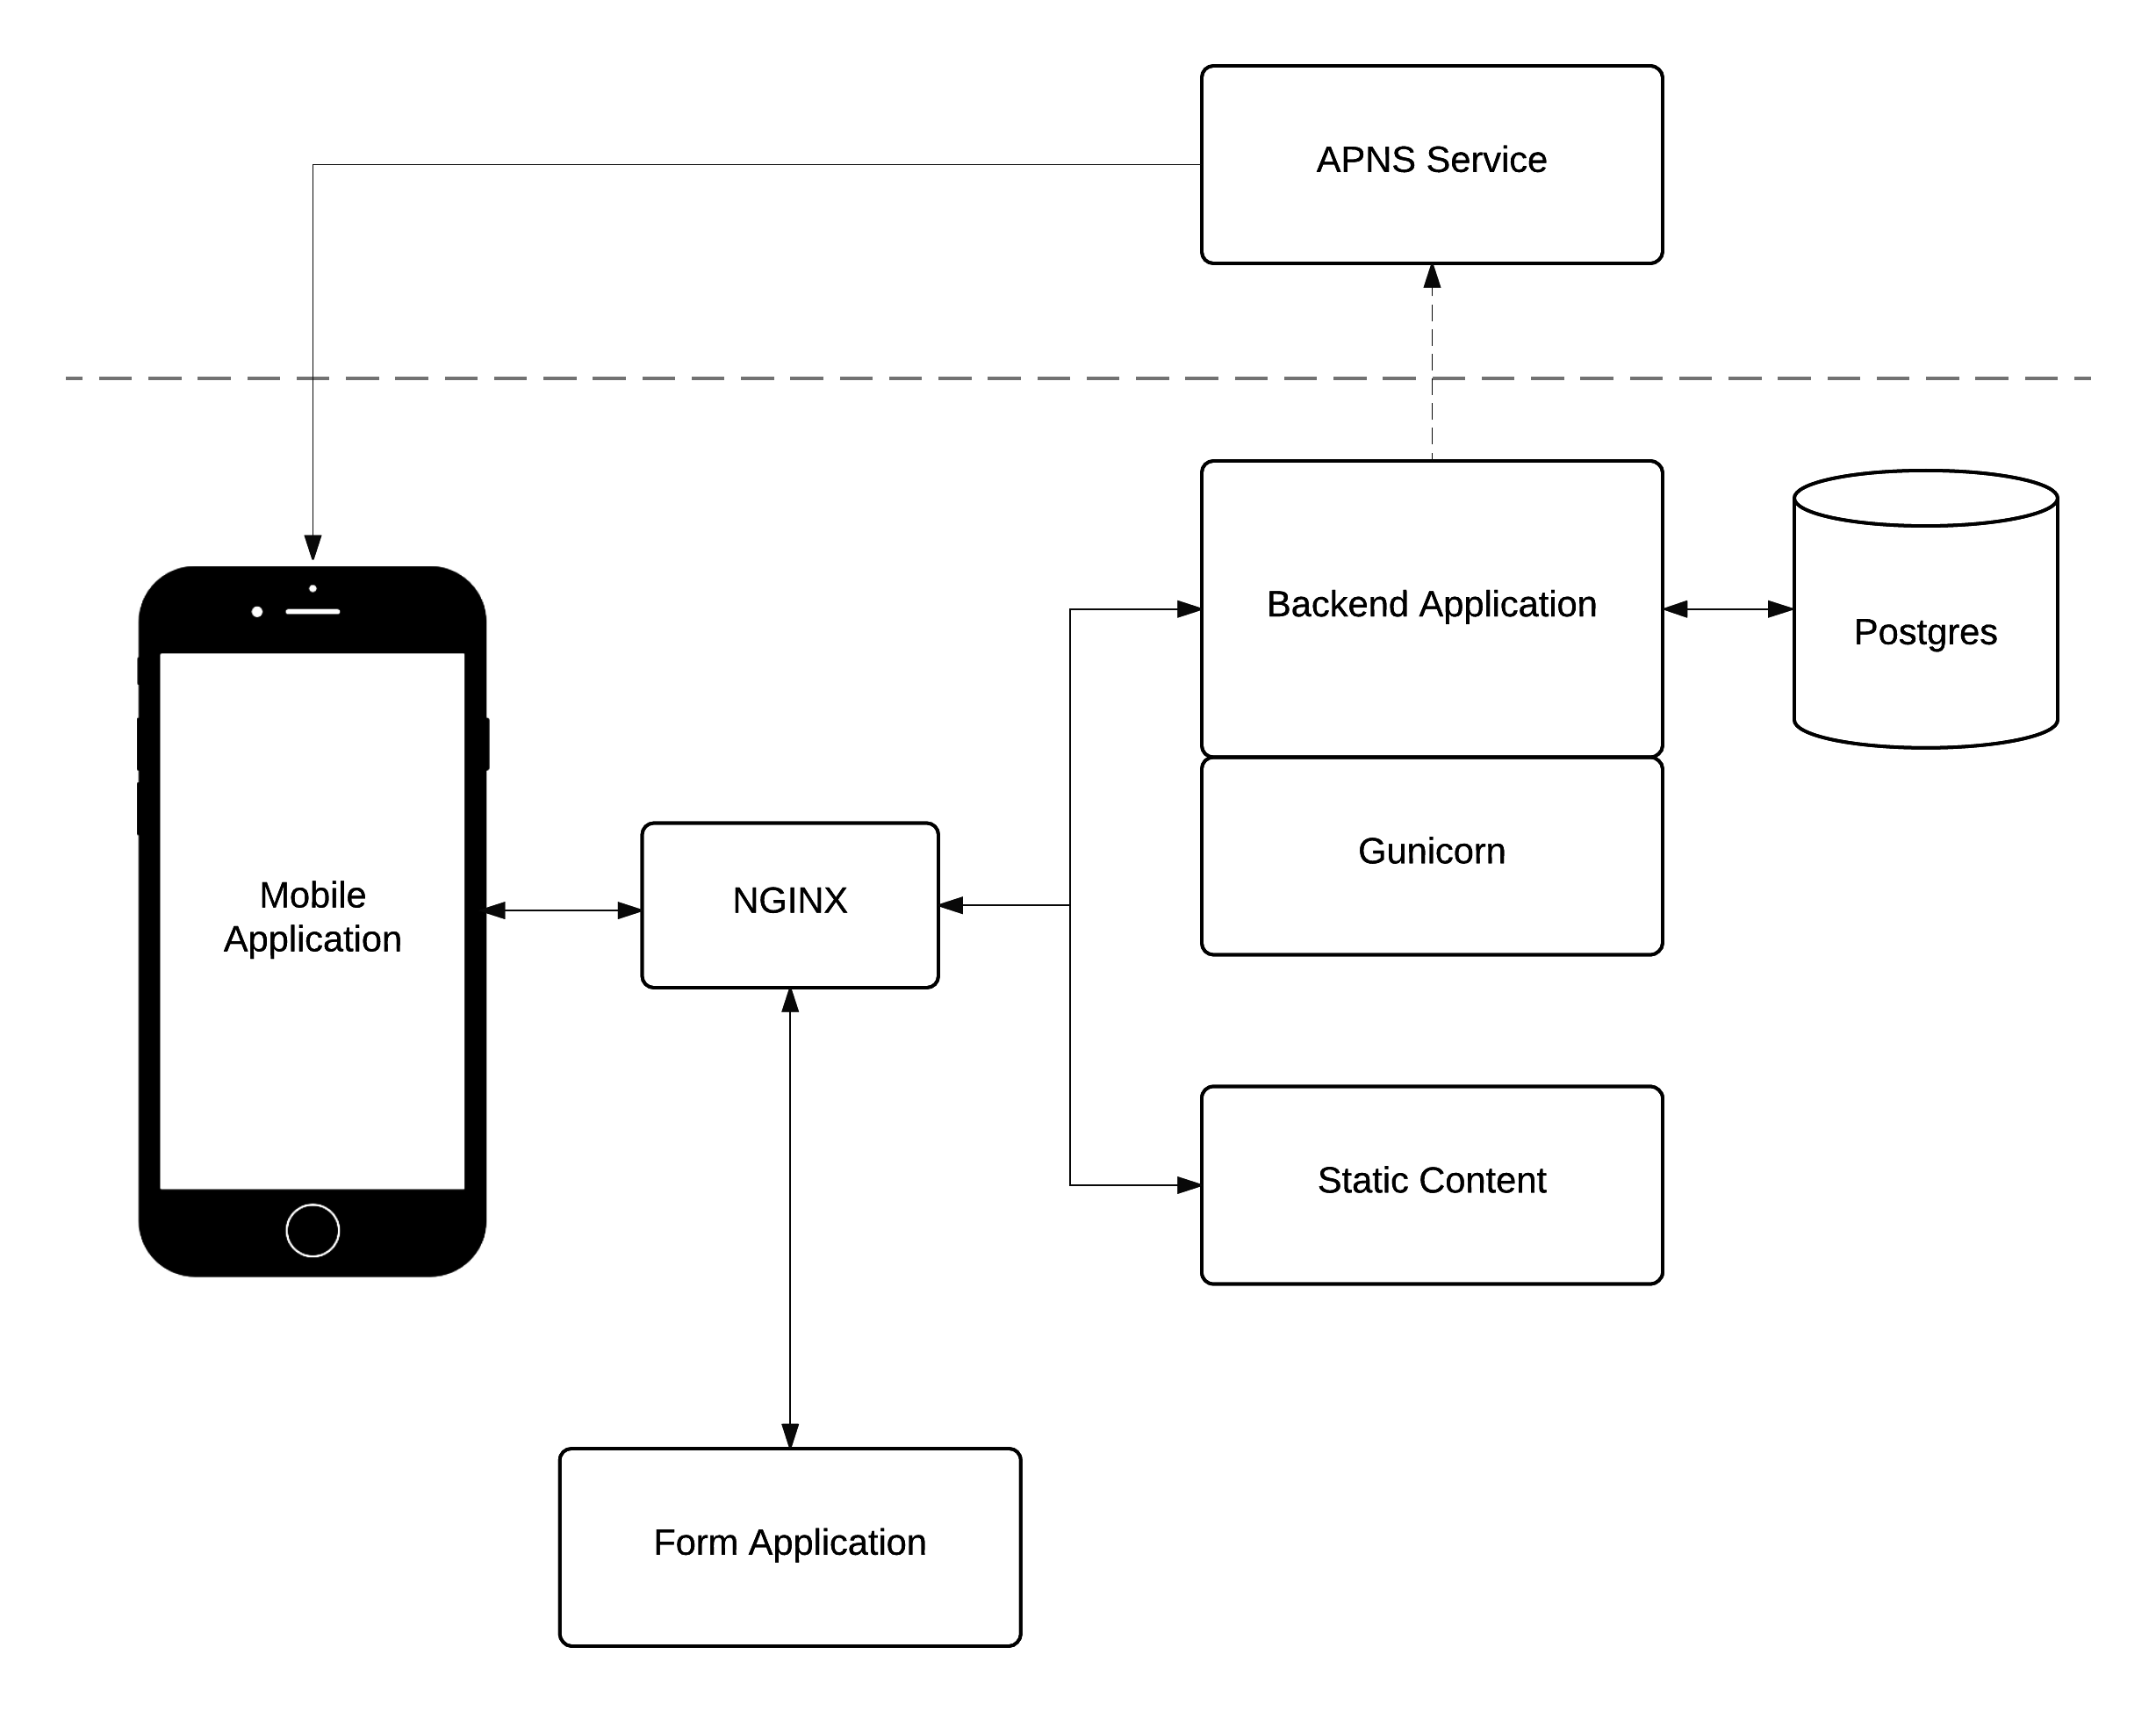
\includegraphics[width=0.7\textwidth]{architecture.png}
  \caption{The diagram shows the overall architecture of TapSensing.} \label{fig:architecture}
\end{figure}

\begin{itemize}
  \item \textbf{Mobile application}: The mobile application provides interfaces for the user to generate taps with corresponding sensor information. Furthermore, the application is capable of sending the acquired data to the backend application. More features of the mobile application are presented in section \ref{sec:mobileapp}. % # TODO
  \item \textbf{NGINX}: For accepting and routing incoming HTTP requests, an NGINX reverse proxy/load balancer is used. The reverse proxy forwards the incoming requests to the server-side application and is capable of serving static content, such as images, HTML, CSS and JavaScript files of the form application.
  \item \textbf{Gunicorn}: Gunicorn is a Python Web Server Gateway Interface (WSGI) HTTP server which runs the source code of the backend application.
  \item \textbf{Backend Application}: The backend application provides HTTP API endpoints which inherit the server-side logic. The backend provides authentication and persistence functionalities. More information on the backend application is to be found in section \ref{sec:backend}
  \item \textbf{PostgreSQL}: TapSensing uses a PostgreSQL\footnote{PostgreSQL is a general purpose and object-relational database management system.} database for storing the application state, user related information, the survey data and the retrieved tap and sensor information.
  \item \textbf{Form application}: The form application provides a web user interface where study participants can answer survey questions.
\end{itemize}

% For the network requests containing the tap information which come from the mobile device to reach the backend, it must first pass through a reverse proxy. As reverse proxy we have chosen NGINX due to it's easy configurability. In this case, NGINX forwards requests to the TapSensing application and serves static files.\\
% The TapSensing backend is written upon the Python Django Framework\footnote{https://www.djangoproject.com/} which is being executed upon the gunicorn application server. Django uses a so-called ORM to perform transactions with the Database, which in our case is a PostgreSQL database.

\section{Mobile Application}
Mobile
\label{sec:mobileapp}

\subsection{User Interface}
\subsubsection{Login}
When the application is opened for the first time, a login screen appears. As in standard login screens, the interface asks for credentials including username and password. Authenticating users, has the advantage, that the generated data can be mapped to individual users.

% The source code of the of the question view is to be found in \texttt{LoginViewController.swift}.

\subsubsection{Start Screen}
During the trial the user is asked to generate taps once a day. In order to indicate if the user is eligible to perform a tap generation trial, the start screen shows a button that is either active or inactive. This switch depends on 4 distinct conditions: \\

\begin{figure}[h!]
  \centering
  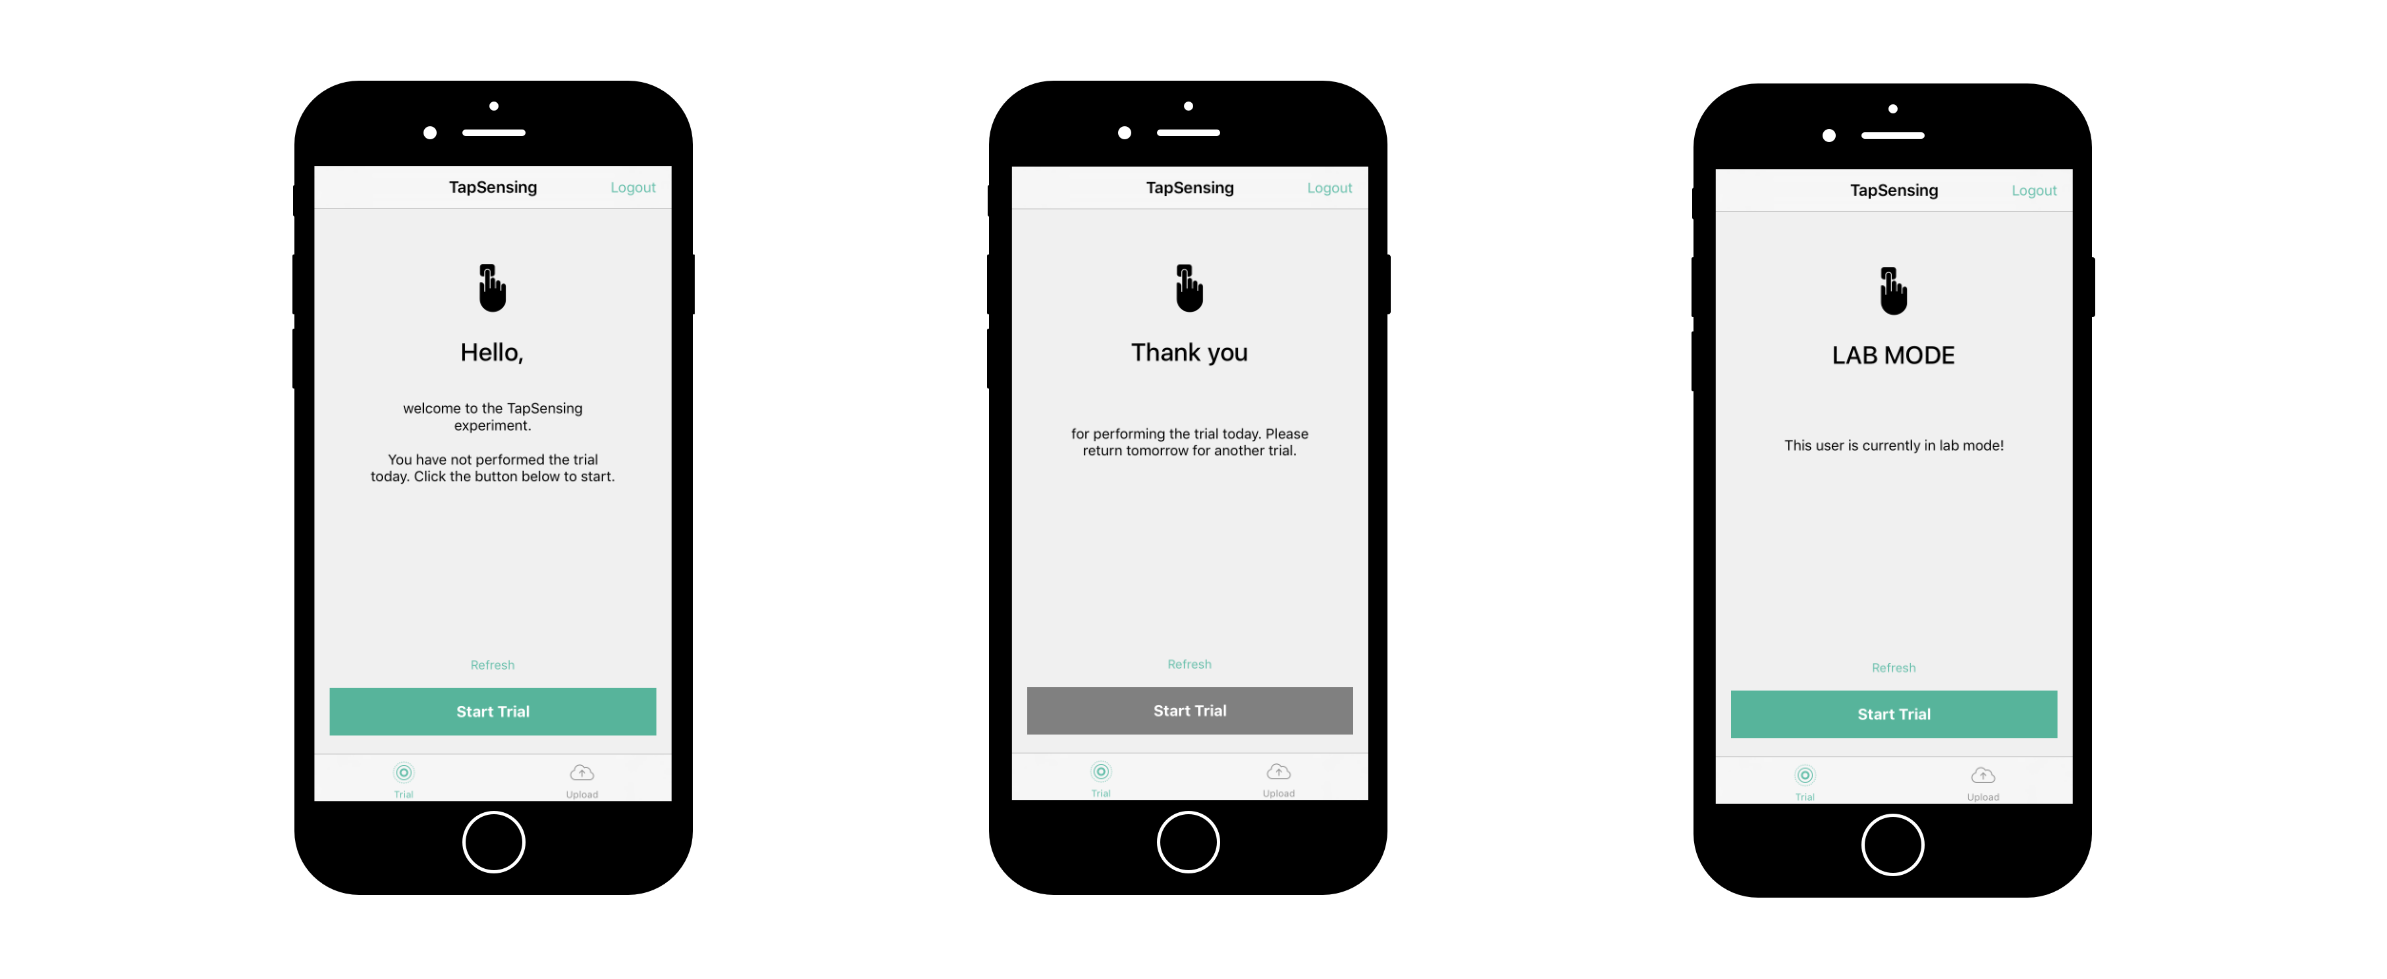
\includegraphics[width=0.8\textwidth]{iphones_startscreen.png}
  \caption{This figure shows the start screen in different configurations. On the left hand-side screenshot, the user has not performed a trial while the the middle image shows the screen where a trial has been performed. The right-hand side image shows the \textit{lab mode} where trails can permanently be performed.}
\end{figure}

When data is collected in the laboratory environment, the app is set to \textit{lab mode}. In \textit{lab mode} the button is always active and trials can be performed. When a user has not performed a trial today, the button is inactive. In contrast, when a user has performed a trial today, the button is inactive and a further trial can be performed the next day. Once all field trials are performed, the app confirms that all data is collected and the button remains inactive.

% The source code of the of the question view is to be found in \texttt{StartViewController.swift}.
\subsubsection{Tap Input}

\begin{figure}[h!]
  \centering
  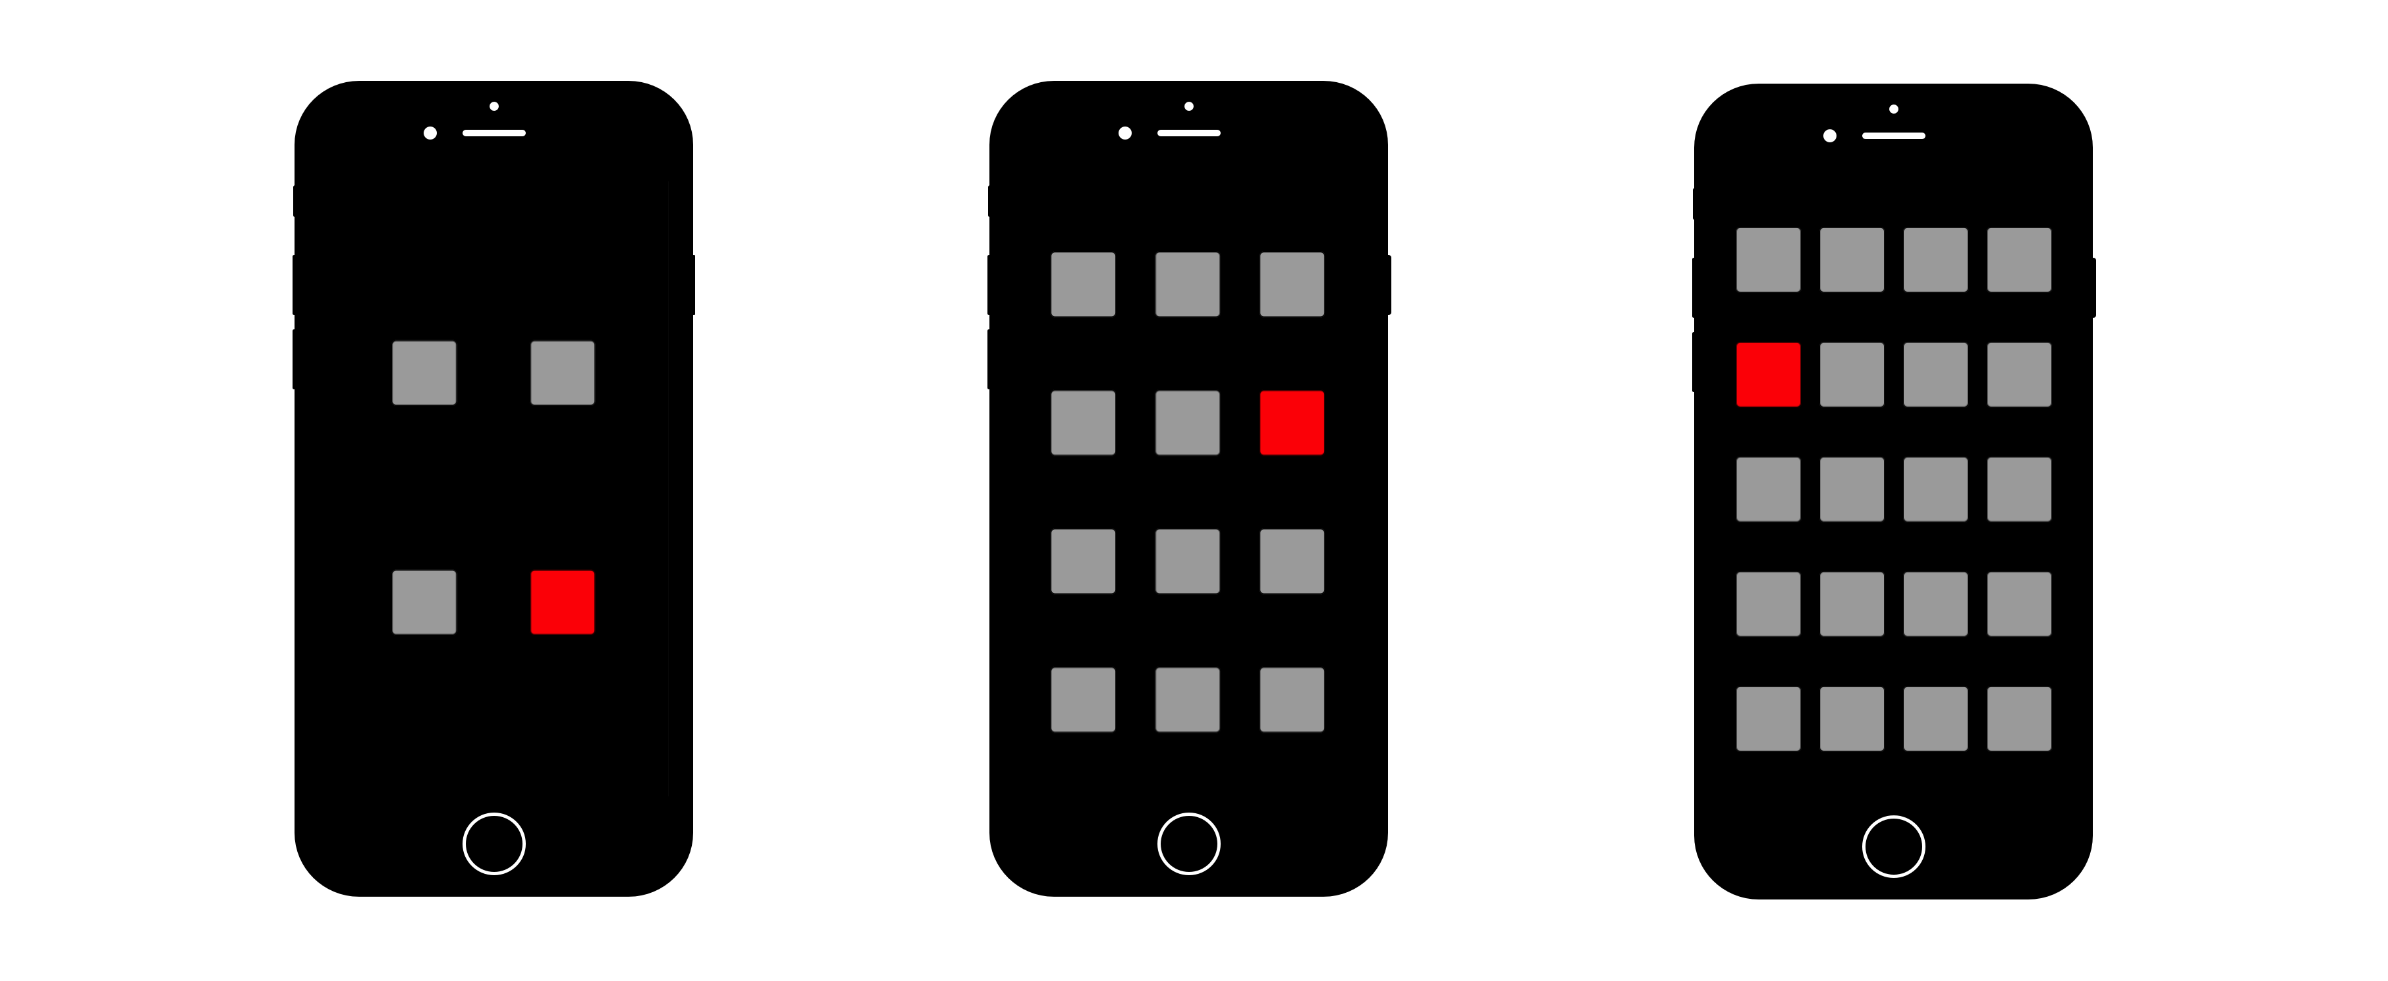
\includegraphics[width=0.8\textwidth]{grids_iphone.png}
  \caption{The figure shows the tap input user interface with buttons aligned in a grid shape structure. The leftmost structure offers 4 buttons, the middle offers 12 buttons whereas displays 20 distinguishable buttons.}\label{fig:grid}
\end{figure}

To acquire individual user taps the mobile application offers a user interface where buttons are aligned in a grid shape structure. The structure is calculated based on a specific configuration set where the amount the vertical and horizontal buttons in the interface can be set. Figure \ref{fig:grid} shows the interface, where 4, 12 and 20 distinguishable buttons are configured.\\

For the user to tap on every location of the screen exactly once, a red button indicating the next button to tap is highlighted guiding the user through the interaction process. While the user is tapping the grid, the gyroscope and accelerometer information is recorded. After all buttons gave been tapped, either a new grid is loaded or the tap acquisition phase ends proceeding with the question interface.

% Maybe a table
% \begin{itemize}
% \item 2 x 2
% \item 4 x 3
% \item 4 x 5
% \end{itemize}

% \begin{center}
%     \begin{tabular}{ | l | l | l | }
%     \hline
%     \# & height & width \\ \hline
%     1 & 2 & 2 \\
%     2 & 4 & 3 \\
%     3 & 4 & 5 \\
%     \hline
%     \end{tabular}
% \end{center}

% The source code of the of the tap input view is to be found in \texttt{GridViewController.swift}.


\subsubsection{Questions}
\begin{figure}[h!]
  \centering
  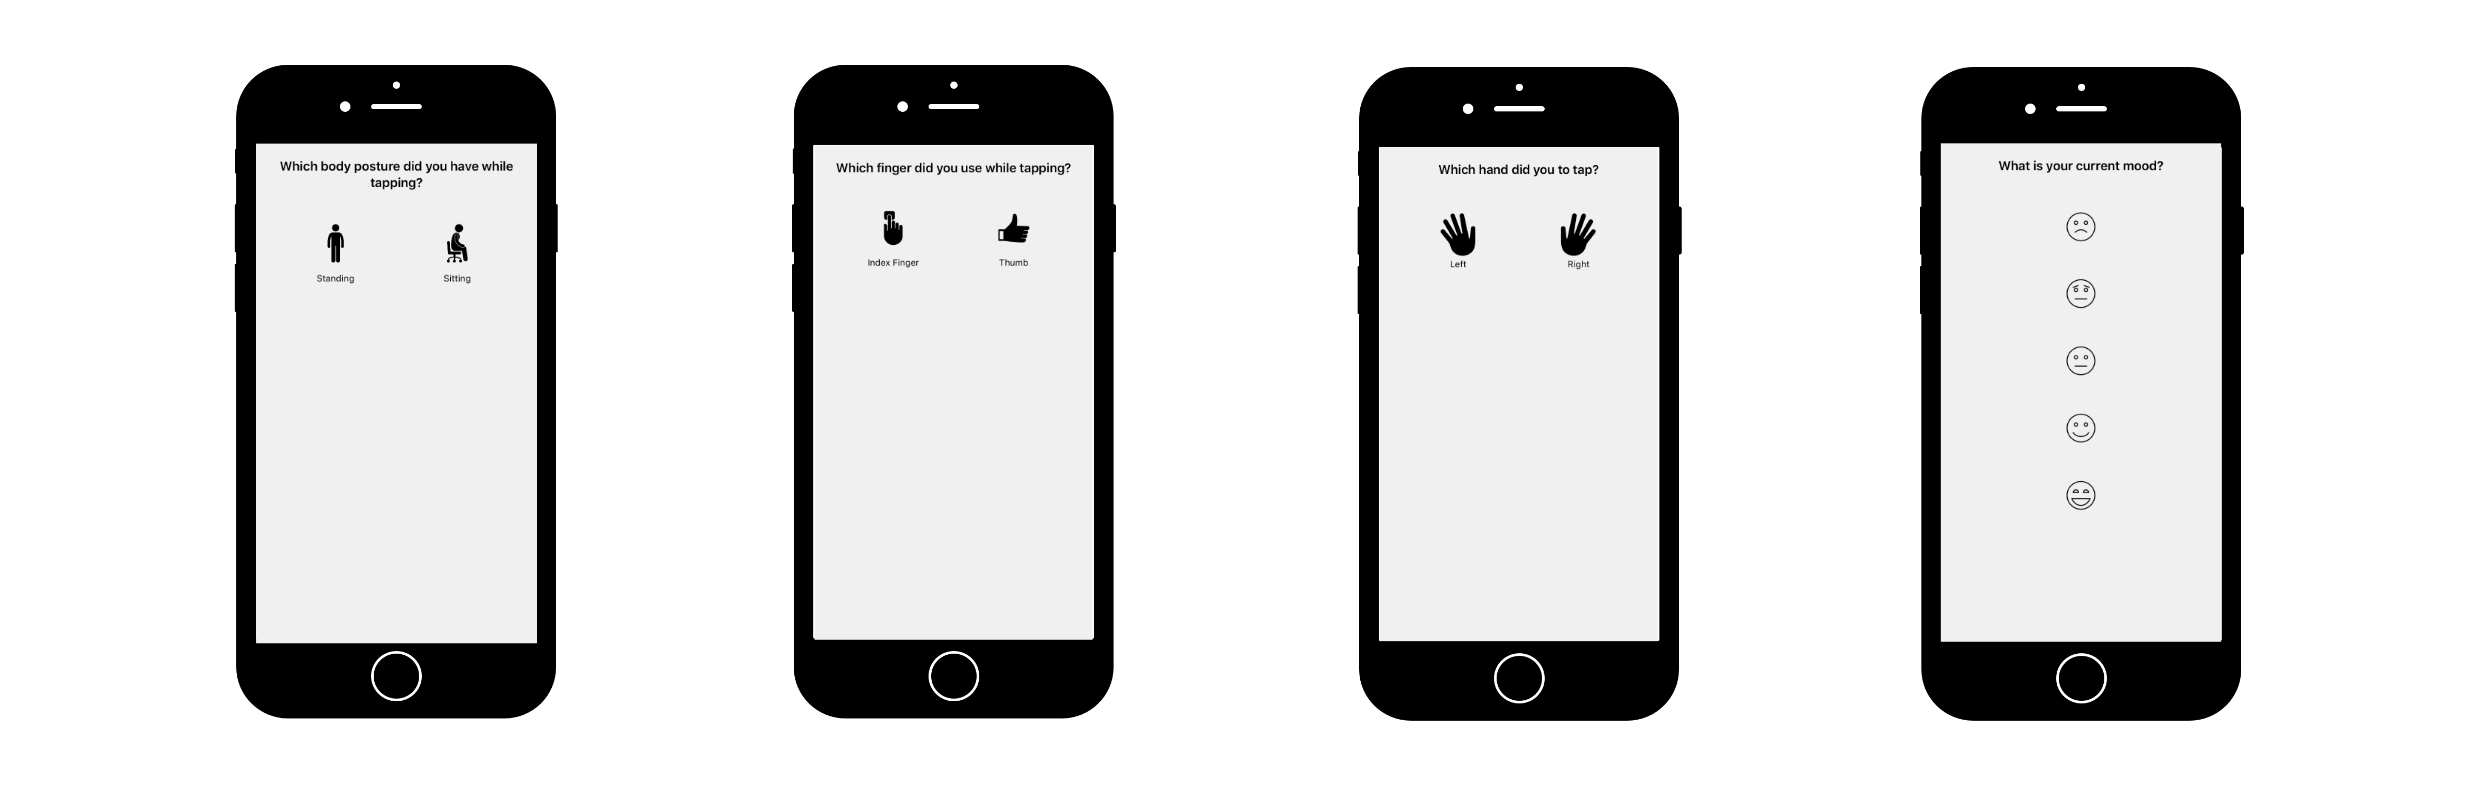
\includegraphics[width=1\textwidth]{questions_iphone.png}
  \caption{The figure displays question views with icons as answer possibilities.}
\end{figure}

To furthermore label the data acquired in the tap input interface, the application provides screens for the user to answer several questions. These question regard the various condition in which the user has generated taps. In the table below the asked questions with corresponding answer choices are to be found.

\begin{center}
  \begin{tabular}{| l | l | l | l |}
  \hline
  \textbf{Question} & \textbf{Answer Choices} \\ \hline
  Which body posture was used during the interaction ? & Standing, Sitting \\
  Which finger did you use while tapping? & Index Finer, Thumb \\
  Which hand did you use to tap? & Left, Right \\
  What is your current mood? & 1 - 5 \\
  \hline
  \end{tabular}
  \caption{The Table shows the questions asked in the question view.}
\end{center}

To enable fast interactions, each answer possibility to a question is represented in the interface with an icon. Once an icon has been pressed, the application transits to the next question until all questions have been answered.

% The source code of the of the question view is to be found in \texttt{QuestionViewController.swift}.

\subsubsection{Upload}
After all taps and questions are gathered, the acquired data is sent to the server. The interface at this points displays a spinning wheel for the user to acknowledge that the mobile phone is processing the data. In case an upload fails, the application provides a manual upload screen, where past sessions can be uploaded.

% The source code of the of the upload views are to be found in \texttt{UploadViewController.swift} and  \texttt{ManualUploadViewController.swift}.
% \subsection{Smartphone Sensors}
% Modern smartphones come with a variety of different sensors offering valuable services to it's users and enhancing many applications. The newest Apple iPhone to date, the iPhone 7, has a fingerprint sensor, a barometer, a three-axis gyroscope and accelerometer (MEMS), a proximity sensor and an ambient light sensor attached to it's main-board \cite{iphone7techspecs}. As we are going to predict finger taps on the iPhone screen, the only sensors that are effected by the force of the tap are the gyroscope and the accelerometer. Therefore, these will be outlined in the following sections.

% \subsubsection{Accelerometer}

% The accelerometer is a sensor module that measures the acceleration it encounters by either movement or gravity \cite{sensorsstudy}. However, the acceleration caused by movement, the so-called inertial acceleration and the gravitational acceleration can not be distinguished by the sensor. This is due to Einstein's equivalence principal stating that the effects of gravity on an object are indistinguishable from the acceleration of the object's reference frame \cite{doi:10.1021/ed014p49.2}. \\

% \begin{figure}[h!]
%   \centering
%   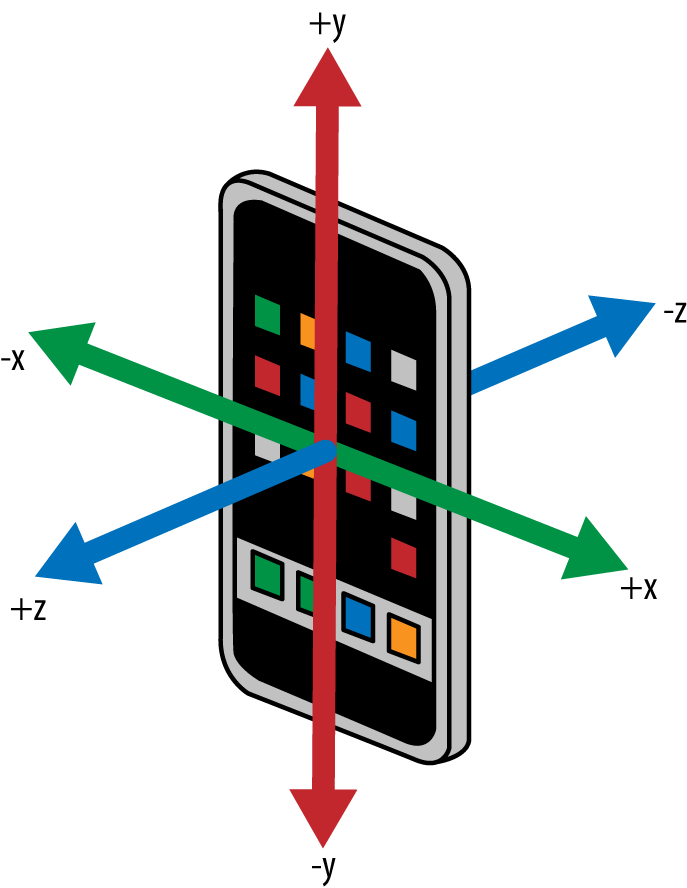
\includegraphics[width=0.35\textwidth]{iphone-acc.png}
%   \caption{Apple iPhone with the corresponding axes of the accelerometer.}
% \end{figure}

% When the position of the device is fixed, as for example when it is placed on a table the accelerometer values would yield $a = \{ a_x = 0, a_y = 0, a_z = -1\}$. This feature make it suitable for detecting device screen rotations. As the device flips from landscape to portrait orientation, the gravity is sensed by a different set of accelerometer axis \cite{sensorsstudy}.\\

% The values of the acceleration are quantified in the SI unit metres per second per second ($m/s^2$). However, in engineering the acceleration is typically expressed in terms of the standard gravity ($g$).

% \subsubsection{Gyroscope}

% As the accelerometer is suitable for detecting orientations, it lacks the ability to detect spin or more precise rotation movements. These spin movements are detected by the gyroscope sensor which is responsible for detecting and maintaining orientation \cite{sensorsstudy}. \\

% A mechanical gyroscope typically composes of a spinning wheel which is set within three so-called gimbals. These gimbals enable the spinning wheel to be set in any orientation. Although the orientation does not remain fixed when the device is rotated, it changes in response to an external torque much lesser and in a different direction than it would be without the large angular momentum associated with it. Each gimbals translates to one of the three gyroscope outputs, namely \textit{pitch}, \textit{roll} and \textit{jaw} (See \cite{wiki:Gyroscope}). \\

% The gyroscope sensor within the MEMS\footnote{Microelectromechanical systems}, the chip deployed in the iPhone, is between 1 to 100 micrometers of size. When the gyroscope is rotated, a small resonating mass is shifted as the angular velocity changes. This movement is converted into very low-current electrical signals that can be amplified and read by a host system. \\

% The values of the gyroscope are quantified in as rotations per seconds (RPS) or as degrees per second ($\deg/s$).

% \subsubsection{Accessing sensor values}
% % Apple offers api for accessing these values.
% In order to access gyroscope and accelerometer Apple provides a high level API\footnote{An Application Program Interface is a set of rules and subroutines provided by an application system for the developer to use. Here is a link to the Core Motion API Documentation: \url{https://developer.apple.com/documentation/coremotion/} } for accessing the device's sensors: \texttt{Core Motion}. Core Motion reports motion and environmental related data from sensors including accelerometers, gyroscopes, pedometers, magnetometers, and barometers in easy to use manner. \\

% Sensor values can either be accessed as proceeded version including aggregations of the values and a raw version. For TapSensing, we make sure to record the raw values to avoid any form of bias. The update interval can be configures at ranges from $10$Hz - $100$Hz. Higher update-rates are possible but are not ensured to be processed in real-time by the device. For TapSensing, the update rate is configured with the highest (safe) value possible. This ensures that tap patterns are captured with an accurate resolution to make a later classification easier. The figure below is a code snipping depicting how sensor values are retrieved in the TapSensing application.

% \begin{figure}[thp]
% \centering
% \begin{minipage}{0.7\textwidth}

% \begin{minted}{swift}
% let UPDATE_INTERVAL = 0.01
% let motionManager = CMMotionManager()

% // Set the update interval on both sensors
% motionManager.gyroUpdateInterval = UPDATE_INTERVAL
% motionManager.accelerometerUpdateInterval = UPDATE_INTERVAL

% // Start reading the sensor values
% motionManager.startAccelerometerUpdates()
% motionManager.startGyroUpdates()

% // Pass in a function to handle sensor update values,
% // which arrive in the update interval rate.
% motionManager.startAccelerometerUpdates(to: .bg) {
%     (data: CMAccelerometerData?, error: Error?) in
%     // handle incoming data
%     ...
% }
% motionManager.startGyroUpdates(to: .bg) {
%     (data: CMGyroData?, error: Error?) in
%     // handle incoming data
%     ...
% }
% \end{minted}
% \end{minipage}
% \caption{Swift code snippet displaying how to access sensor values with Core Motion.}
% \label{test}
% \end{figure}

\subsection{Implementation Notes}
\subsubsection{Obtaining Sensor Information}
In order to access the gyroscope and the accelerometer, Apple provides a high-level API\footnote{An Application Program Interface is a set of rules and subroutines provided by an application system for the developer to use. The following link leads to the Core Motion API documentation: \url{https://developer.apple.com/documentation/coremotion/} } for accessing the device's sensors: \textit{Core Motion}. Core Motion provides motion and environmental related data from sensors including accelerometers, gyroscopes, pedometers, magnetometers, and barometers in easy to use manner. \\

Sensor values can either be accessed as proceeded including aggregations of the values or as raw version. For TapSensing, raw values are recorded to avoid any form of bias. The update interval can be configures at ranges from $10$Hz - $100$Hz. Higher update-rates are possible but are not ensured to be processed in real-time by the device. For TapSensing, the update rate is configured with the highest (safe) value possible. This ensures that tap patterns are captured with high resolution in order to make a classification easier.
\subsubsection{Local Persistence}
It is possible that a session upload fails due to lack of internet access or another reason. Due to this, the application stores all session information and sensory data in it's local SQLite database. For local persistence Apple provides it's own framework called \textit{Core Data} which is extensively used in TapSensing. Once the data has been successfully received by the backend, the data is deleted from the local database.
\subsubsection{Push Notifications}
TapSensing is registered with the Apple Push Notification Service allowing the application to receive push notifications. Notifications are used to remind the user during the field study, that he has to take part in the study.
\subsubsection{Distribution}
Installing iOS applications that are not uploaded to the Apple App Store, requires each device to be registered in the Apple Developer Portal with the smartphone's serial number. To avoid this, the application has been uploaded to the App Store enabling an easy distribution.

\section{Backend application}
\label{sec:backend}
\subsection{HTTP Endpoints}
\label{sec:endpoints}
For the purpose of interoperability the network communication from the mobile application and the forms application to the server-side application is done via HTTP Requests in the JSON\footnote{JSON (JavaScript Object Notation)\cite{ietf-jsonbis-rfc7159bis-04} is a lightweight data-interchange format.} format. The endpoints listed below represent tiny logic components that can be called from an external client.
\begin{center}
  \begin{tabular}{|p{2cm}|p{4cm}|p{8cm}|}
  \hline
  \textbf{HTTP \newline Method} & \textbf{URL} & \textbf{Description} \\ \hline
  POST & /login & Provides login functionalities for the mobile client. This method returns an authentication, that is used for further requests to authenticate the user.\\
  \hline
  POST & /session & Provides upload functionality for a session data objects.\\
  \hline
  POST & /touchevent & Provides upload functionality for touchevent data objects.\\
  \hline
  POST & /sensordata & Provides upload functionality for a sensordata data objects.\\
  \hline
  POST & /apns & Retrieves the Device's APNS token. This is required to send push notifications to the users.\\
  \hline
  GET & /trial-settings & Provides the configuration for the tap input view. Here, the amount of buttons and the amount of grid repetitions that are to be performed in a single session can be defined.\\
  \hline
  POST & /survey & Provides upload functionalities for the survey form application.\\
  \hline

  \end{tabular}
  \caption{The Table shows the questions asked in the question view.}
\end{center}

\subsection{Data Model}
TapSensing's data model reflect the schemas that are used in the PostgreSQL database. As seen in figure \ref{fig:erdiagram}, the data model consists of 4 data objects that I will describe in this section:

\begin{itemize}
  \item \textbf{User}: The user model is inherited by the Django's user model\footnote{For more information on the Django user model, the following URL leads to the model's documentation: \url{https://docs.djangoproject.com/en/1.11/ref/contrib/auth/}}. The user model is used for authentication and persisting the authentication token. The other models described in this section are connected to the user model through a foreign key relation to identify the user associated with the data object.
  \item \textbf{Session}: The session data object holds all information associated with the user's trial. This includes the data collecting in the ``labeling part''\footnote{The ``labeling part refers to the question views, where additional information on the data acquired is collected'''} of the application such as the hand used, the body posture and the typing modality. In addition, information is stored such as device infos and if the session took place in a laboratory or field environment.
  \item \textbf{Touchevent}: The touchevent data object stores information regarding the ``ground truth'' of the user generated tap including the exact x and y coordinates, timestamp and an identifier of the specific grid rectangle tapped in the tap input view. Furthermore, it is noted if the user hit a specific rectangle and if the event is a touch-down or touch-up event.
  \item \textbf{Sensordata}: The sensordata data object captures all information obtained by the gyroscope and accelerometer of the mobile device. To differentiate between accelerometer and gyroscope values, the data object includes a type field. In addition, the model captures the timestamp and the 3-sensor components (x, y, z) of the individual sensors.
\end{itemize}

\begin{figure}[h!]
  \centering
  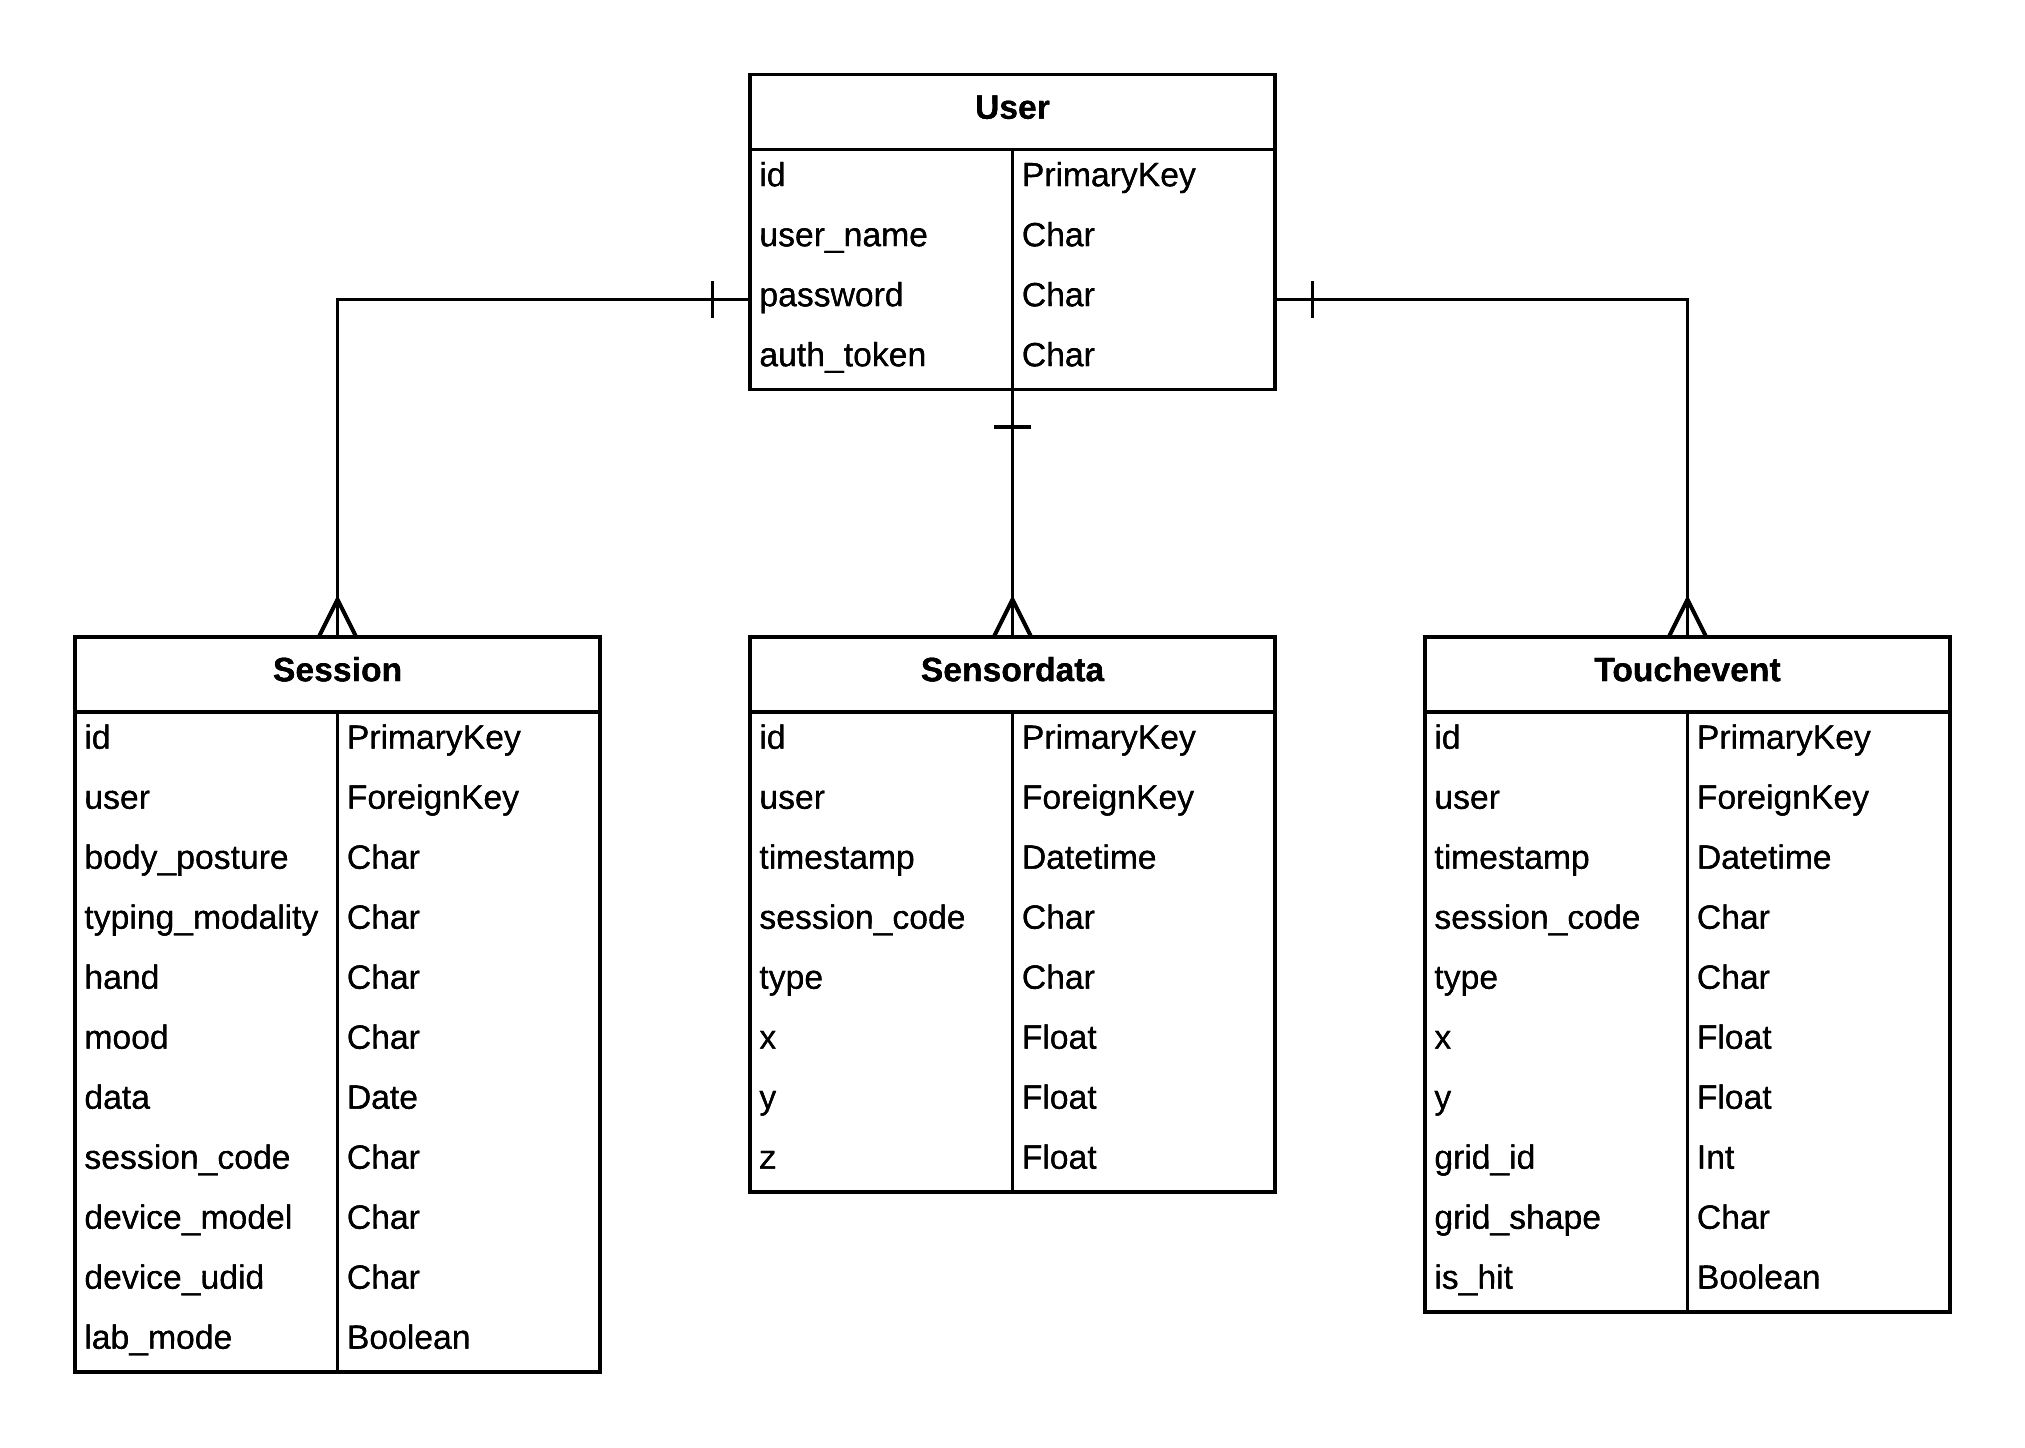
\includegraphics[width=1\textwidth]{datamodel1.png}
  \caption{The diagram shows TapSensing's data model with the user, session, sensordata and touchevent data object.} \label{fig:erdiagram}
\end{figure}

% An additional model was created for the survey application.

% \begin{figure}[h!]
%   \centering
%   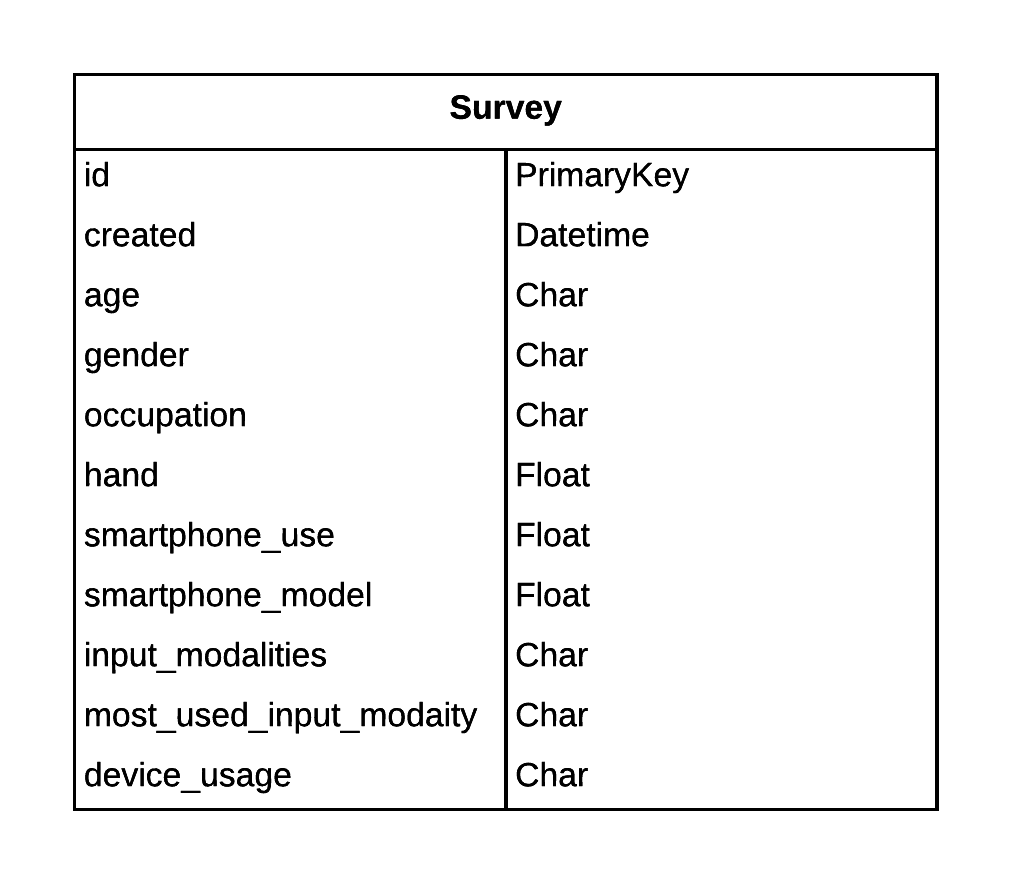
\includegraphics[width=0.4\textwidth]{datamodel2.png}
%   \caption{The diagram shows TapSensing's data model with the user, session, sensordata and touchevent data object.} \label{fig:erdiagram}
% \end{figure}

\subsection{Implementation Notes}
\subsubsection{Authentication}
The authentication mechanism implemented in TapSensing is based on a standard token authentication scheme. This allows the association of an incoming request with a set of identifying credentials, which is - in this context - the user the request came from. In order to obtain an authentication token, the mobile application sends the login credentials of a user including username and password to the login endpoint\footnote{The login endpoint is described in section \ref{sec:endpoints}.}. When the credentials have been checked for validity, the endpoints returns an authentication token in the following format:
\begin{minted}[tabsize=4]{js}
{     
  "token": "Token 3acc6c2a58723e2f1579d4526add2511f6a0a525"
}
\end{minted}
The token is then added to the HTTP request in the ``Authorization'' header to authenticate the user.
\subsubsection{Ensuring data consistency}



\subsubsection{Push Notifications}
Participants are reminded every day with push notifications during the field study to take part as previous research has shown that push notifications greatly enhance the participation \cite{pushNot}. In the same study\cite{pushNot}, passive notifications - notifications without sound - have been seen to positively impact the user taking action. Following these assumptions, a push notification strategy has been implemented combining notifications with and without sound. Figure \ref{fig:push-notifications} shows the implemented strategy with trigger times. \\

\begin{figure}[h!]
  \centering
  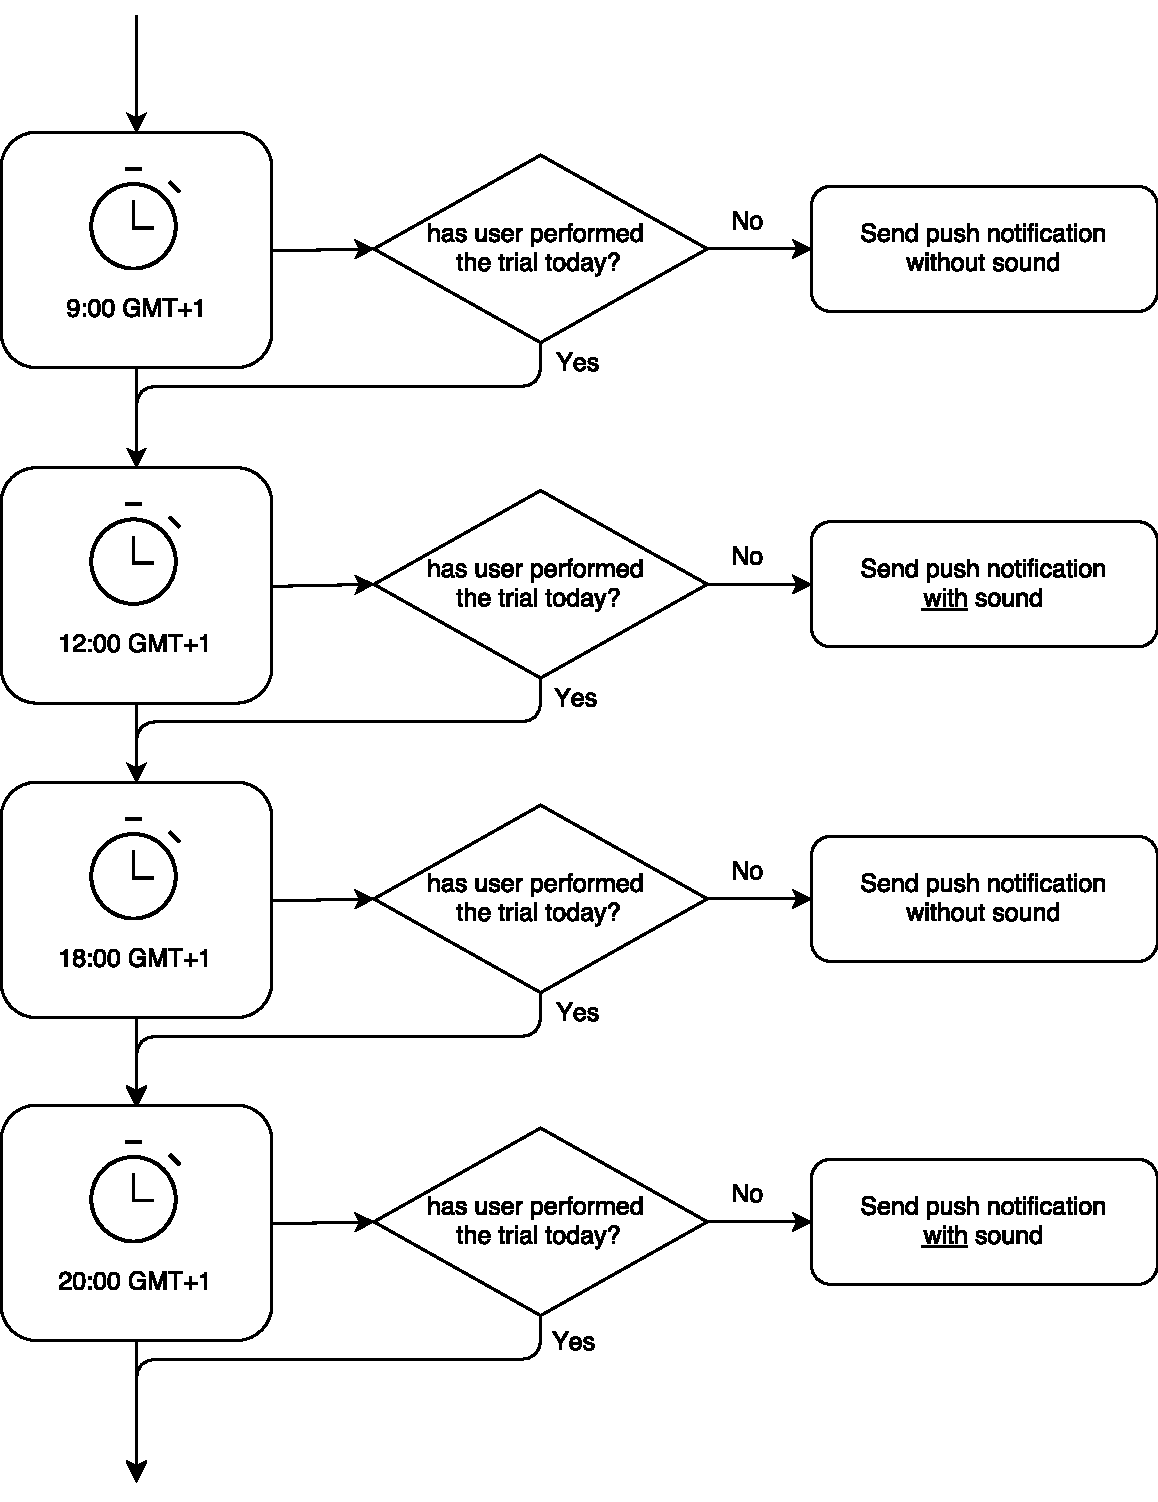
\includegraphics[width=0.5\textwidth]{push_notifications.pdf}
  \caption{The diagram shows the implemented push notification strategy.} \label{fig:push-notifications}
\end{figure}

Implementation-wise, the Django package \textit{django-push-notifications}\footnote{\url{https://github.com/jleclanche/django-push-notifications}} is used providing mechanisms to register devices as well as to send notifications.
\subsubsection{Backups}
To prevent data loss, the PostgreSQL database is backed up via a unix cronjob every evening. The database dumps are sent automatically to Amazon Web Services S3 Bucket.
\subsubsection{Deployment}

    \chapter{Data Preprocessing \label{cha:chapter4}}
\section{Overview}
1. Query 2. Split into Taps 3. Interpolate 4. Feature Extraction 5. CSV
\section{Feature Extraction}
- Explain column, matrix and sensor features.

\begin{figure}[h!]
  \centering
  \begin{minipage}{.3\textwidth}
    \centering
    \begin{tikzpicture}
      \matrix [matrix of math nodes] (m)
      {
          g_{x_0} &g_{x_1} &g_{x_2} &g_{x_3} &g_{x_4} \\
          g_{y_0} &g_{y_1} &g_{y_2} &g_{y_3} &g_{y_4} \\            
          g_{z_0} &g_{z_1} &g_{z_2} &g_{z_3} &g_{z_4} \\
          \_ & \_ & \_ & \_ & \_ \\      
          a_{x_0} &a_{x_1} &a_{x_2} &a_{x_3} &a_{x_4} \\
          a_{y_0} &a_{y_1} &a_{y_2} &a_{y_3} &a_{y_4} \\            
          a_{z_0} &a_{z_1} &a_{z_2} &a_{z_3} &a_{z_4} \\
      };
      \draw[color=black!100, thick] (m-1-1.north west) -- (m-1-5.north east) -- (m-1-5.south east) -- (m-1-1.south west) -- (m-1-1.north west);
      \draw[color=black!100, thick] (m-2-1.north west) -- (m-2-5.north east) -- (m-2-5.south east) -- (m-2-1.south west) -- (m-2-1.north west);
      \draw[color=black!100, thick] (m-3-1.north west) -- (m-3-5.north east) -- (m-3-5.south east) -- (m-3-1.south west) -- (m-3-1.north west);
      \draw[color=black!100, thick] (m-5-1.north west) -- (m-5-5.north east) -- (m-5-5.south east) -- (m-5-1.south west) -- (m-5-1.north west);
      \draw[color=black!100, thick] (m-6-1.north west) -- (m-6-5.north east) -- (m-6-5.south east) -- (m-6-1.south west) -- (m-6-1.north west);
      \draw[color=black!100, thick] (m-7-1.north west) -- (m-7-5.north east) -- (m-7-5.south east) -- (m-7-1.south west) -- (m-7-1.north west);
      \node[align = center, below=2cm]{Column Features};
    \end{tikzpicture}
  \end{minipage}
  \begin{minipage}{.3\textwidth}
    \centering
    \begin{tikzpicture}
      \matrix [matrix of math nodes] (m)
      {
          g_{x_0} &g_{x_1} &g_{x_2} &g_{x_3} &g_{x_4} \\
          g_{y_0} &g_{y_1} &g_{y_2} &g_{y_3} &g_{y_4} \\            
          g_{z_0} &g_{z_1} &g_{z_2} &g_{z_3} &g_{z_4} \\
          \_ & \_ & \_ & \_ & \_ \\      
          a_{x_0} &a_{x_1} &a_{x_2} &a_{x_3} &a_{x_4} \\
          a_{y_0} &a_{y_1} &a_{y_2} &a_{y_3} &a_{y_4} \\            
          a_{z_0} &a_{z_1} &a_{z_2} &a_{z_3} &a_{z_4} \\
      };
      \draw[color=black!100, thick] (m-1-1.north west) -- (m-1-5.north east) -- (m-3-5.south east) -- (m-3-1.south west) -- (m-1-1.north west);
      \draw[color=black!100, thick] (m-5-1.north west) -- (m-5-5.north east) -- (m-7-5.south east) -- (m-7-1.south west) -- (m-5-1.north west);      
      \node[align = center, below=2cm]{Sensor Features};     
      % \draw[color=black,8oublies-](m-1-2.north) -- +(0,0.3);
    \end{tikzpicture}
  \end{minipage}
  \begin{minipage}{.3\textwidth}
    \centering
    \begin{tikzpicture}
      \matrix [matrix of math nodes] (m)
      {
          g_{x_0} &g_{x_1} &g_{x_2} &g_{x_3} &g_{x_4} \\
          g_{y_0} &g_{y_1} &g_{y_2} &g_{y_3} &g_{y_4} \\            
          g_{z_0} &g_{z_1} &g_{z_2} &g_{z_3} &g_{z_4} \\
          \_ & \_ & \_ & \_ & \_ \\      
          a_{x_0} &a_{x_1} &a_{x_2} &a_{x_3} &a_{x_4} \\
          a_{y_0} &a_{y_1} &a_{y_2} &a_{y_3} &a_{y_4} \\            
          a_{z_0} &a_{z_1} &a_{z_2} &a_{z_3} &a_{z_4} \\
      };
      \draw[color=black!100, thick] (m-1-1.north west) -- (m-1-5.north east) -- (m-7-5.south east) -- (m-7-1.south west) -- (m-1-1.north west);
      % \draw[color=red,double,implies-](m-1-2.north) -- +(0,0.3);
      \node[align = center, below=2cm]{Matrix Feature};
    \end{tikzpicture}
  \end{minipage}
  \caption{The figure shows how different features are extracted from the overall sensor matrices: Column features, sensor features and matrix features.}
\end{figure}  

\subsection{Column Features}
\begin{center}
  % Feature Description
  \begin{tabular}{ | l| l | l | l |}
  \hline
  Name & Description & Feature Type & Amount \\
  \hline
    \texttt{peak} & Amount of peaks in the time series & column  & 6 \\
    \texttt{zero\_crossing} & Amount of zero crossings in the signal & column  & 6 \\ 
    \texttt{energy} & Energy of the signal & column  & 6 \\ 
    \texttt{entropy} & Entropy measure of the the signal & column  & 6 \\
    \texttt{mad} & Median absolute deviation of the signal & column  & 6 \\
    \texttt{ir} & Interquartile Range & column  & 6 \\
    \texttt{rms} & Root mean square of the signal & column  & 6 \\
    \texttt{mean} & Mean of the time series & column  & 6 \\
    \texttt{std} & Standard deviation of the time series & column  & 6 \\
    \texttt{min} & Minimum of the time series & column  & 6 \\
    \texttt{median} & Median of the time series & column  & 6 \\
    \texttt{max} & Maximal value of the time series & column  & 6 \\
    \texttt{var} & Variance of the time series & column  & 6 \\
    \texttt{skew} & Skewness of the time series & column  & 6 \\
    \texttt{kurtosis} & Kurtosis of the time series & column  & 6 \\
    \texttt{sem} & Standard error of the time series & column  & 6 \\
    \texttt{moment} & Moment in the time series & column & 6 \\
    \texttt{spline} & Spline interpolation of the signal (12 steps) & column  & 6*12 \\
  \hline
    \texttt{fro\_norm} & Frobenius matrix norm & matrix & 1 \\
    \texttt{inf\_norm} & Infinity matrix norm & matrix & 1 \\
    \texttt{l2\_norm} & L2 matrix norm & matrix & 1 \\
  \hline
    \texttt{cos\_angle} & Cosine Angle of sensor component pairs & sensor & 3 \\
    \texttt{pears\_cor} & Pearson Correlation of sensor component pairs & sensor & 3 \\
    
  \hline
  \end{tabular}
\end{center}

% peak,
% zero_crossing,
% energy,
% entropy,
% mad,
% iqr,
% rms,
% np.mean,
% np.std,
% np.min,
% np.median,
% np.max,
% np.var,
% st.skew,
% st.kurtosis,
% st.sem,
% st.moment
\subsection{Matrix Features}
\begin{center}
  % Feature Description
  \begin{tabular}{ | l | l |}
  \hline
  Name & Description \\
  \hline
    \texttt{fro\_norm} & - \\
    \texttt{inf\_norm} & - \\
    \texttt{l2\_norm} & - \\
  \hline
  \end{tabular}
\end{center}
\subsection{Sensor Features}
\section{Feature Scaling}

    \chapter{Method\label{cha:chapter5}}

\section{Hypothesis}
To recall, in the related work section previous research was presented showing that PIN\footnote{Personal Identification Number} and passwords can be obtained by reconstructing touchscreen taps based on motion sensor readings \cite{Tapprints, Accessory, Touchlogger}. However, since the data in these approaches was collected in a controlled environment, it has not been shown that the feasibility to predict tap locations also applies to a more natural environment where users usually engage with their personal smartphones. This question forms the first hypothesis of this thesis.

\begin{center}
  \begin{mdframed}[backgroundcolor=gray!10] 
    \textbf{H1}  The environment of recorded sensor data has an effect on the prediction accuracy.
  \end{mdframed}
\end{center}

\begin{center}
  \begin{framed}
    \textbf{H1.1:} The prediction accuracy for a classifier trained with the laboratory data will score higher than one trained with the field data.
  \end{framed}
\end{center}

Furthermore, 

\begin{center}
  \begin{mdframed}[backgroundcolor=gray!10]
    \textbf{H2:} The input modality has an effect on the prediction accuracy.
  \end{mdframed}
\end{center}

It is plausible that typing with the index finger and holding the device in the other hand will cause less movement of the smartphone as typing with a thumb will. This is presumably to be reflected in the motion data.

\begin{center}
  \begin{framed}
    \textbf{H2.2:} The prediction accuracy for a classifier trained with index finger tap data will score higher than one trained with thumb tap data.
  \end{framed}
\end{center}

Moreover, I presume that 
\begin{center}
  \begin{framed}
    \textbf{H3:} The body posture has an effect on the prediction accuracy.
  \end{framed}
\end{center}

Similar to the input modality, it is also plausible that a user that taps a smartphone screen while sitting will move lesser than standing.

\begin{center}
  \begin{framed}
    \textbf{H2.2:} The prediction accuracy for a classifier trained with index finger tap data will score higher than one trained with thumb tap data.
  \end{framed}
\end{center}


\begin{center}
  \begin{framed}
    \textbf{H1.1:} The prediction accuracy for a classifier trained with the laboratory data will score higher that one trained with the field data for each of the three grids.
  \end{framed}
\end{center}

\section{Experimental Approach}

\begin{figure}[h!]
  \centering
  \includegraphics[width=1\textwidth]{process.pdf}
  \caption{This figure shows the overall appraoch to the experiment.} \label{fig:appraoch}
\end{figure}

The overall experiment consists of a three step process. In the first step, labeled data is acquired from subjects invited to take part in the experiment. For this purpose, the TapSensing application presented in the last chapter is used. The data acquisition part is necessary to collect sensor data with the corresponding ground truth of the tap locations for the supervised learning task. 

After the data is successfully acquired, the continuos sensor recordings are preprocessed to obtain the portion of recording which represents each individual tap. To extract certain characteristics of the sensor signature created by the each tap, feature are extracted in a further step. These features are then used to train a set of classifiers. 

The classification results are then discussed in the results section of this work.
% TODO: statistical test.

% - Data acquisition
%   - Ground truth of the touch Environments with grid_id and timestamps
%   - Sensory recordings of gryoscope and accelerometer
%   - input modalities and body posture
%   - Environments Lab and field
% - Preprocessing Feature Extraction


\section{Labeled Data Acquisition}

\subsection{Subjects}
A total of 27 subjects were invited to participate in the study. There were no restrictions concerning the demographics of individual subjects. However, each subjects had to be in  possession of one of the permitted iOS devices.

\subsection{Devices}
The devices have been restricted to the Apple iPhone 6, 6s and 7 based on their mutual screen size. Furthermore, as the screen size has a large effects on the sensor signature created by a tap, the screen size is an important factor to enable the comparison of classification results among devices.

\subsection{Environments \& Conditions}
As the study aimed at collecting sensor reading both in the field as well as in a laboratory environment, the data acquisition is done in two distinct settings:
\begin{enumerate}
  \item \textbf{Laboratory Evironment}: Subjects were invited to a laboratory room which had a standard office ergonomics setup. Subjects have been asked to either sit at the desk or stand in the room while tapping.
  \item \textbf{Field Environment}: Subjects were asked to generate taps using their smartphone at any place they are currently located. For example, this could be at home, at work or during leisure activity.
\end{enumerate}

Besides the environment of the recorded sensor data, the collected varies in the input modality and body posture while the tap was made. Subjects are either allowed to use the index finger (while holding the device in the other hand) or the thumb to generate taps. Sitting and Standing are allowed as body postures as these two represent the natural interactions with the smartphone. 

\subsection{Acquisition Procedure}
In order for participants to generate tap data, the subjects were invited to come to the laboratory for the first part of the experiment. To avoid information asymmetry, each participant read an experiment instruction\footnote{The instruction sheet is to be found in the appendix.}. Subjects should then confirm whether they have understood the previously read information. Additional questions regarding the instructions were answered. In the next step, subjects were asked to fill out an online questionnaire regarding their persona and personal smartphone usage.

% TODO: instruction in appendix
To begin with the data acquisition, participants were asked to download the application from the Apple App Store and to login using provided credentials.

\begin{figure}[h!]
  \centering
  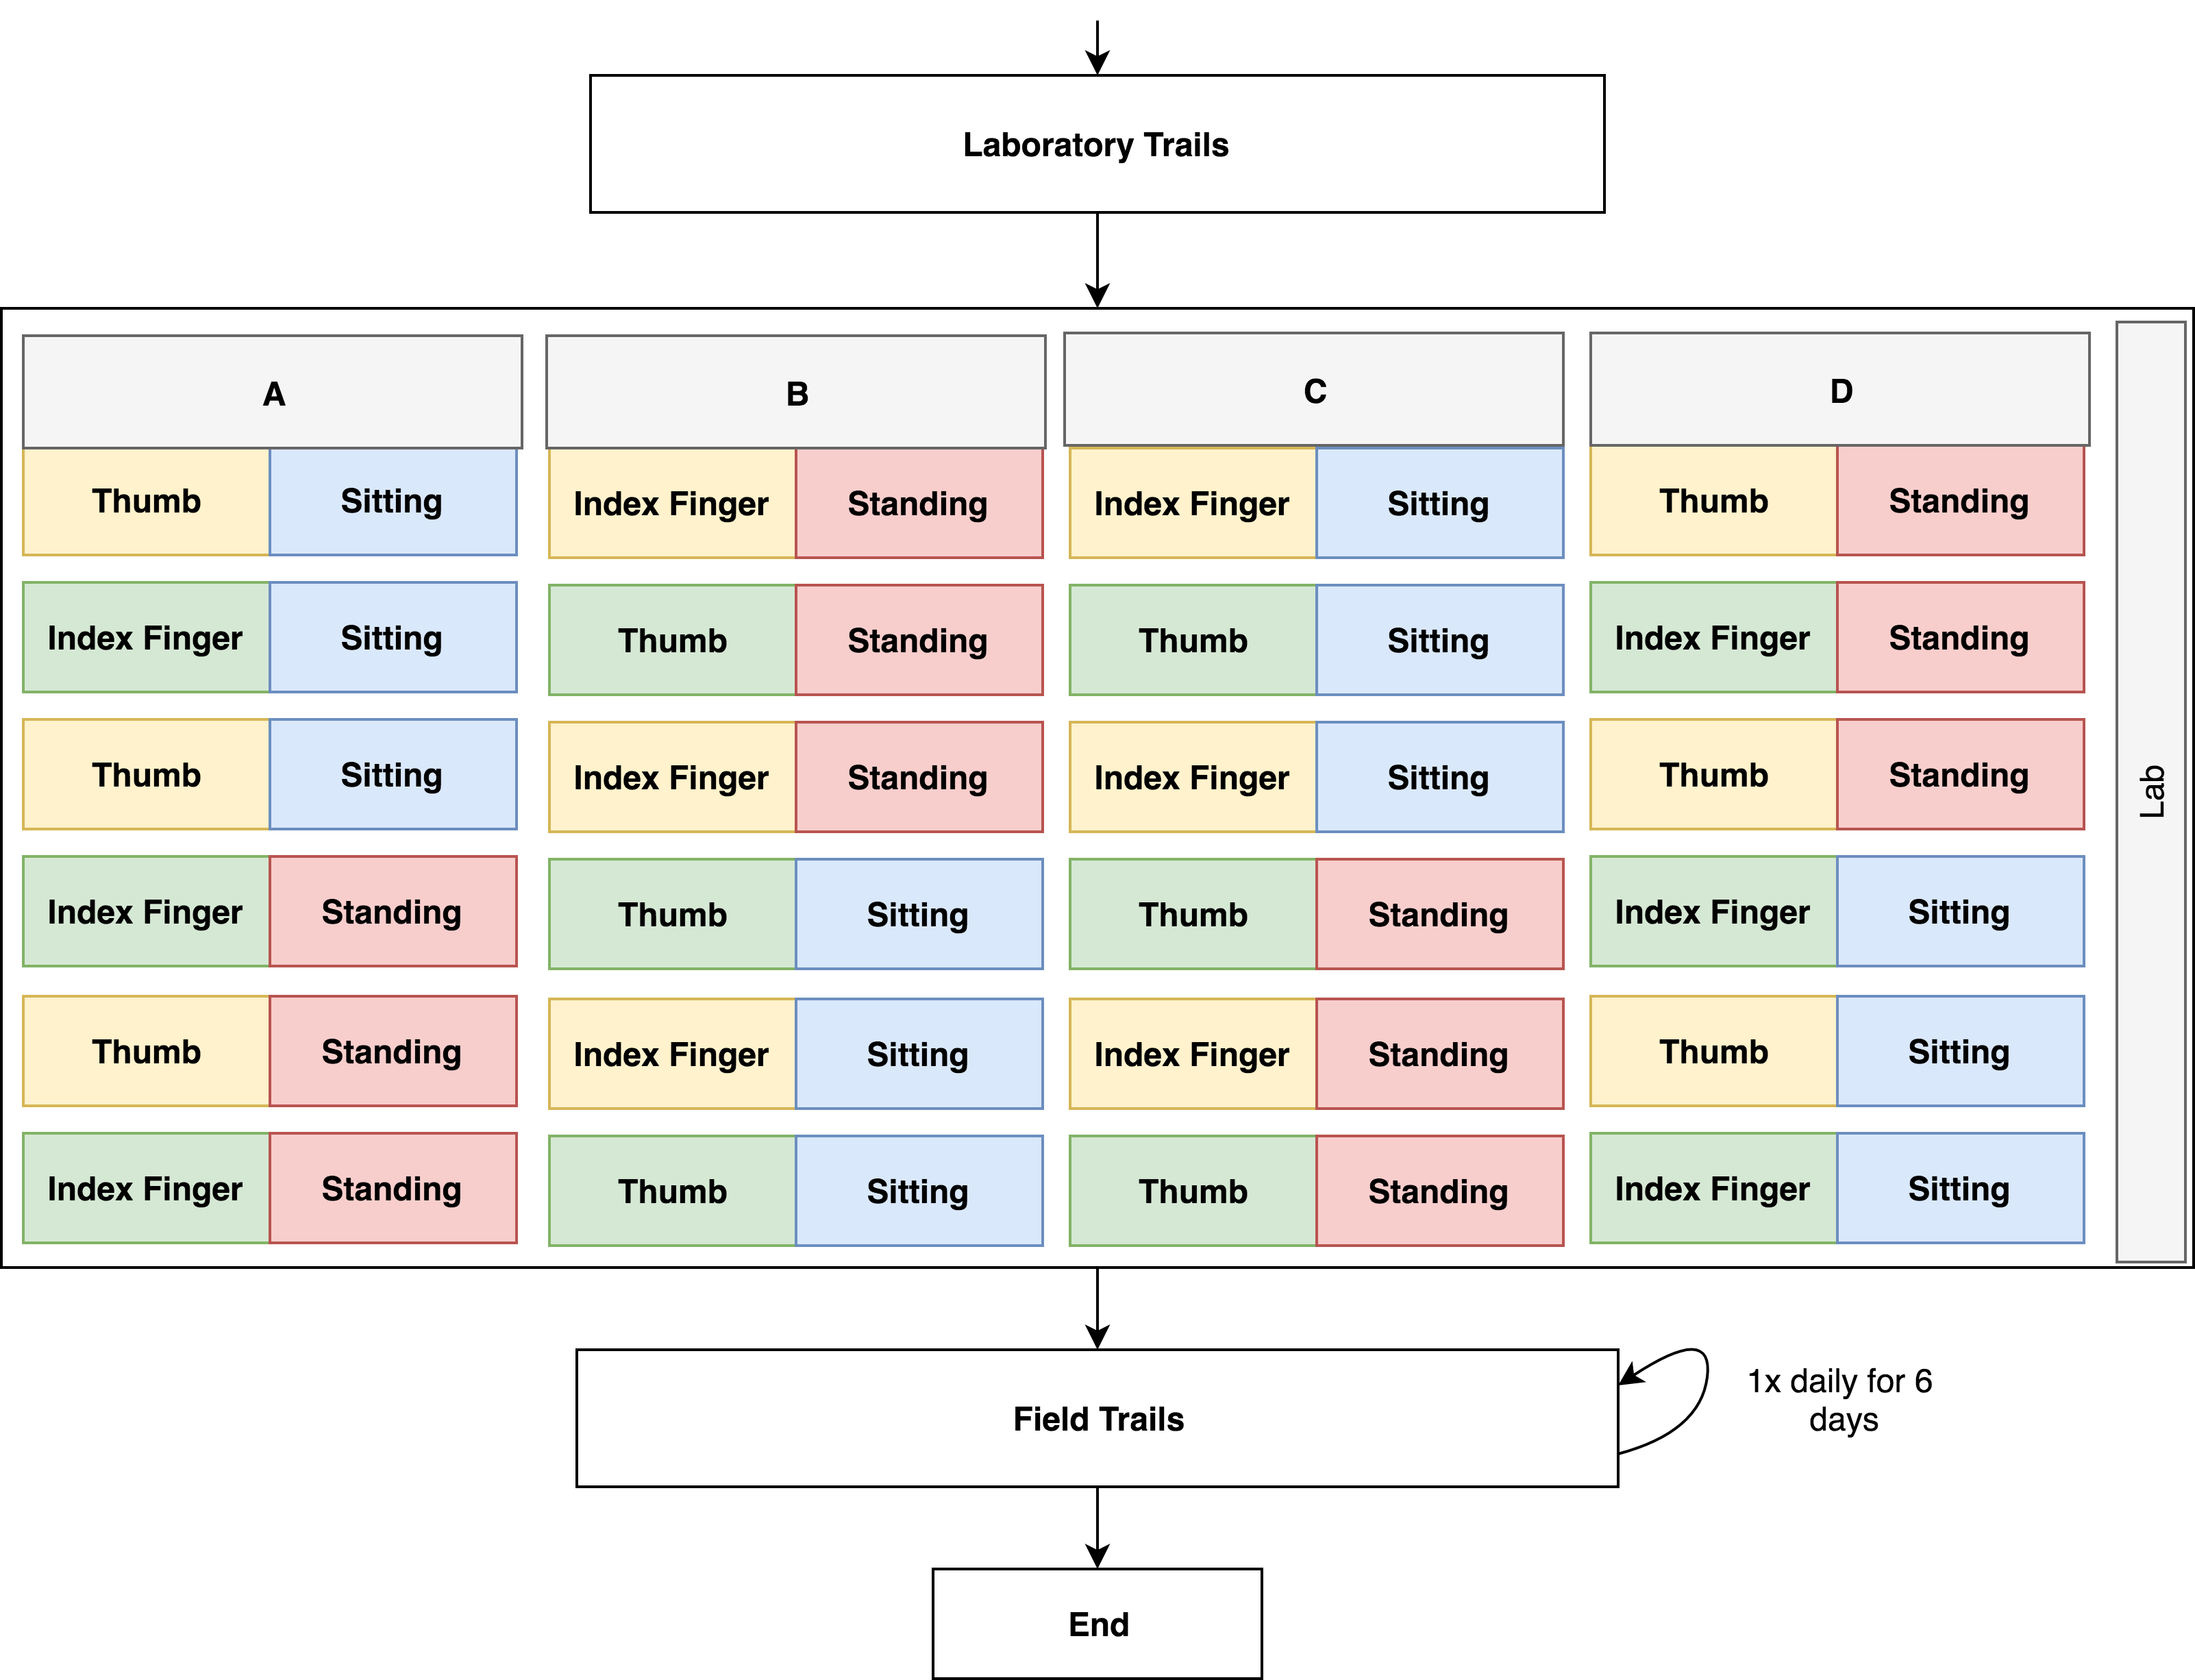
\includegraphics[width=1\textwidth]{study_design.png}
  \caption{This figure shows the procedure every subject has to perform in the study.} \label{fig:study_design}
\end{figure}

Subsequently, subjects were asked to perform 6 consecutive trials in the TapSensing application, whereas one trail includes tapping each grid four times in randomized order. Recall, the grid sizes defined consist of 4, 12 and 20 distinguishable buttons. For an equal distribution of the body posture and the input modality while tapping, each trial is dependent on one of four configurations onto which each subject is assigned. These configuration are to be seen in Figure \ref{fig:study_design}.  It is important to note that each subject is not allowed to alter the body posture or input modality during a trial. After all trials are performed, subjects were asked to continue with the field study.\\

During the field study, subjects performed one trial daily on 6 separate days. On each day push notifications were sent as a reminder to participate. Subjects were free to decide which input modality or body posture to use as the aim of the field study is to collect data that represents regular smartphone usage.

\section{Data Preprocessing \label{cha:chapter4}}
\subsection{Preprocessing}
Before features can be extracted from individual taps, the continuous sensor recording from each trial needs to be sliced to obtain the portion of the recordings which is relevant for the tap. The timestamp of the touchdown event is used to find an appropriate starting point. Here, 20ms are subtracted from the timestamp as due to the latency between the physical touchdown event and the recorded event. Based on the data collected in the pilot study, the average tap duration (being the duration between a touchdown and the corresponding touchup event) between 70ms - 200ms. Taking this value into account, a window size of 150ms was chosen to enrich each slice with more information. Figure \ref{fig:touchdown} shows the sensor components of a gyroscope reading with a slicing window marked with a grey background. 

\begin{figure}[h!]
  \centering
  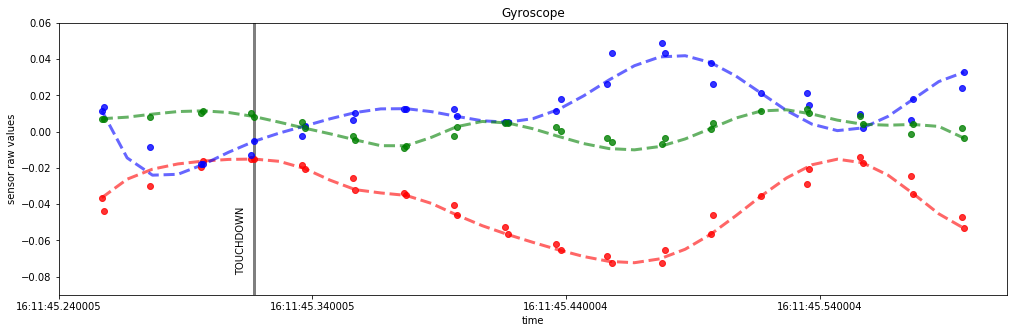
\includegraphics[width=1\textwidth]{gyroscope_touchdown.png}
  \caption{The figure shows a continuos gyroscope reading with the slicing window and corresponding timestamps. The timestamp of the touchdown event is used as an anchor point.} \label{fig:touchdown}
\end{figure}

Unfortunately, due to different CPU loads on the mobile devices, sensor values are not pushed from the operating system to the mobile application in a constant manner leading to an uneven distribution of the sensor recordings on the time scale. To balance out each tap to a fixed amount of values, a cubic spline interpolation is used. Figure \ref{fig:touchdown} shows the interpolated sensor components with dots representing the raw recordings. Furthermore, recordings that are below 75Hz are filtered out. After the slices are produced for each tap, features are extracted.

\subsection{Feature Extraction}
A feature is an individual measurable property or characteristic of a phenomenon being observed \cite{Duda:2000:PC:954544}. Therefore, choosing discriminant and independent features is a crucial step for the performance of the later classification. Fortunately, \citeauthor{Tapprints}'s preliminary work has shown a comprehensive list of possible sensor features of which the following features are partially adapted.

\begin{figure}[h!]
  \centering
  \begin{minipage}{.3\textwidth}
    \centering
    \begin{tikzpicture}
      \matrix [matrix of math nodes] (m)
      {
          g_{x_0} &g_{x_1} &g_{x_2} &g_{x_3} &g_{x_4} \\
          g_{y_0} &g_{y_1} &g_{y_2} &g_{y_3} &g_{y_4} \\            
          g_{z_0} &g_{z_1} &g_{z_2} &g_{z_3} &g_{z_4} \\
          \_ & \_ & \_ & \_ & \_ \\      
          a_{x_0} &a_{x_1} &a_{x_2} &a_{x_3} &a_{x_4} \\
          a_{y_0} &a_{y_1} &a_{y_2} &a_{y_3} &a_{y_4} \\            
          a_{z_0} &a_{z_1} &a_{z_2} &a_{z_3} &a_{z_4} \\
      };
      \draw[color=black!100, thick] (m-1-1.north west) -- (m-1-5.north east) -- (m-1-5.south east) -- (m-1-1.south west) -- (m-1-1.north west);
      \draw[color=black!100, thick] (m-2-1.north west) -- (m-2-5.north east) -- (m-2-5.south east) -- (m-2-1.south west) -- (m-2-1.north west);
      \draw[color=black!100, thick] (m-3-1.north west) -- (m-3-5.north east) -- (m-3-5.south east) -- (m-3-1.south west) -- (m-3-1.north west);
      \draw[color=black!100, thick] (m-5-1.north west) -- (m-5-5.north east) -- (m-5-5.south east) -- (m-5-1.south west) -- (m-5-1.north west);
      \draw[color=black!100, thick] (m-6-1.north west) -- (m-6-5.north east) -- (m-6-5.south east) -- (m-6-1.south west) -- (m-6-1.north west);
      \draw[color=black!100, thick] (m-7-1.north west) -- (m-7-5.north east) -- (m-7-5.south east) -- (m-7-1.south west) -- (m-7-1.north west);
      \node[align = center, below=2cm]{Column Features};
    \end{tikzpicture}
  \end{minipage}
  \begin{minipage}{.3\textwidth}
    \centering
    \begin{tikzpicture}
      \matrix [matrix of math nodes] (m)
      {
          g_{x_0} &g_{x_1} &g_{x_2} &g_{x_3} &g_{x_4} \\
          g_{y_0} &g_{y_1} &g_{y_2} &g_{y_3} &g_{y_4} \\            
          g_{z_0} &g_{z_1} &g_{z_2} &g_{z_3} &g_{z_4} \\
          \_ & \_ & \_ & \_ & \_ \\      
          a_{x_0} &a_{x_1} &a_{x_2} &a_{x_3} &a_{x_4} \\
          a_{y_0} &a_{y_1} &a_{y_2} &a_{y_3} &a_{y_4} \\            
          a_{z_0} &a_{z_1} &a_{z_2} &a_{z_3} &a_{z_4} \\
      };
      \draw[color=black!100, thick] (m-1-1.north west) -- (m-1-5.north east) -- (m-3-5.south east) -- (m-3-1.south west) -- (m-1-1.north west);
      \draw[color=black!100, thick] (m-5-1.north west) -- (m-5-5.north east) -- (m-7-5.south east) -- (m-7-1.south west) -- (m-5-1.north west);      
      \node[align = center, below=2cm]{Sensor Features};     
      % \draw[color=black,8oublies-](m-1-2.north) -- +(0,0.3);
    \end{tikzpicture}
  \end{minipage}
  \begin{minipage}{.3\textwidth}
    \centering
    \begin{tikzpicture}
      \matrix [matrix of math nodes] (m)
      {
          g_{x_0} &g_{x_1} &g_{x_2} &g_{x_3} &g_{x_4} \\
          g_{y_0} &g_{y_1} &g_{y_2} &g_{y_3} &g_{y_4} \\            
          g_{z_0} &g_{z_1} &g_{z_2} &g_{z_3} &g_{z_4} \\
          \_ & \_ & \_ & \_ & \_ \\      
          a_{x_0} &a_{x_1} &a_{x_2} &a_{x_3} &a_{x_4} \\
          a_{y_0} &a_{y_1} &a_{y_2} &a_{y_3} &a_{y_4} \\            
          a_{z_0} &a_{z_1} &a_{z_2} &a_{z_3} &a_{z_4} \\
      };
      \draw[color=black!100, thick] (m-1-1.north west) -- (m-1-5.north east) -- (m-7-5.south east) -- (m-7-1.south west) -- (m-1-1.north west);
      % \draw[color=red,double,implies-](m-1-2.north) -- +(0,0.3);
      \node[align = center, below=2cm]{Matrix Feature};
    \end{tikzpicture}
  \end{minipage}
  \caption{The figure shows how different features are extracted from the overall sensor matrices: Column features, sensor features and matrix features.}\label{fig:featureextraction}
\end{figure}  

The features extracted are differentiated based on the set of axis where aggregational functions are applied. These can be categorized as column features, sensor features and matrix features, as illustrated in figure \ref{fig:featureextraction}. Column features refer to features that are a product of a function being applied to each \textit{x}, \textit{y} and \textit{z} sensor axis separately. Sensor features are defined as features where sensor axis are combined. An example for a sensor feature is the Pearson correlation which is calculated for each sensor component pair \textit{xy}, \textit{xz} and \textit{yz}. With sensor features, relations between the components are captured. Lastly, matrix features are a product of a function being applied to both gyroscope and accelerometer time series.

Since taps on different locations of the screen generate different sensor signatures we design features that are able to capture the properties of the sensor readings generated by a tap. For this purpose, a total of 230 features have been extracted for each individual tap. The table \ref{table:features} below shows the complete list of features ordered by feature type. Features have been extracted from both the time domain and the frequency domain. In addition, to standardize the range of the features extracted, a Min-Max scaling is applied to each feature.

\begin{center}
  % Feature Description
  \begin{tabular}{ | l| l | l | l |}
  \hline
  Name & Description & Feature Type & Amount \\
  \hline
    \texttt{peak} & Amount of peaks in the time series & column  & 6 \\
    \texttt{zero\_crossing} & Amount of zero crossings in the signal & column  & 6 \\ 
    \texttt{energy} & Energy of the signal & column  & 6 \\ 
    \texttt{entropy} & Entropy measure of the the signal & column  & 6 \\
    \texttt{mad} & Median absolute deviation of the signal & column  & 6 \\
    \texttt{ir} & Interquartile Range & column  & 6 \\
    \texttt{rms} & Root mean square of the signal & column  & 6 \\
    \texttt{mean} & Mean of the time series & column  & 6 \\
    \texttt{std} & Standard deviation of the time series & column  & 6 \\
    \texttt{min} & Minimum of the time series & column  & 6 \\
    \texttt{median} & Median of the time series & column  & 6 \\
    \texttt{max} & Maximal value of the time series & column  & 6 \\
    \texttt{var} & Variance of the time series & column  & 6 \\
    \texttt{skew} & Skewness of the time series & column  & 6 \\
    \texttt{kurtosis} & Kurtosis of the time series & column  & 6 \\
    \texttt{sem} & Standard error of the time series & column  & 6 \\
    \texttt{moment} & Moment in the time series & column & 6 \\
    \texttt{spline} & Spline interpolation of the signal (12 features) & column  & 6*12 \\
    \texttt{fft} & Fast Fourier Transform (5 features) & column  & 6*5 \\
  \hline
    \texttt{cos\_angle} & Cosine Angle of sensor component pairs & sensor & 6 \\
    \texttt{pears\_cor} & Pearson Correlation of sensor component pairs & sensor & 6 \\
  \hline
    \texttt{fro\_norm} & Frobenius matrix norm & matrix & 1 \\
    \texttt{inf\_norm} & Infinity matrix norm & matrix & 1 \\
    \texttt{l2\_norm} & L2 matrix norm & matrix & 1 \\
  \hline
  \end{tabular}
  \captionof{table}{Table of features extracted from every tap.}\label{table:features}
\end{center}

\section{Classification}
After the features are extracted for all the tap data acquired, learning algorithms are applied in order to measure the classification accuracy. In this experiment, a SVM with radial basis kernel is used as well as a feedforward artifical neural network.

\subsection{Evaluation}
To evaluate the classifiers trained in the classification part of the experiment, a K-fold cross-validation is used. In K-fold cross-validation, the training set is divided into K subsets of equal sizes. Sequentially, every subset is tested using the classifier trained on the remaining K-1 subsets. During this process, each pattern in the dataset is predicted once. After K classifiers are trained, the mean of the accuracy scores is computed to determine how well the classifier performs.

\subsection{Grid Search}
In order to optimize the hyperparameters of each learning algorithm, a grid search is performed. A grid search is an exhausting search through a defined subset of the hyperparameter space for each algorithm. The subset of parameters are combined using the cartesian product in order to configure the classifier. To evaluate the each classifier with a set of hyperparameters, a 5-fold cross validation is performed.

The parameters $C$ and $\gamma$ of the SVM RBF kernel are tested during the grid search using exponential growing sequenced, a recommended method to find suitable parameters \cite{hsu2003practical}.
\begin{align}
  C &= \{ 2^{k} | k \in \{-3, -2, ..., 14, 15\} \}\\ 
  \gamma &= \{ 2^{k} | k \in \{-13, -12, ..., 2, 3\} \}
\end{align}
As for the SVM, hyperparameters are defined for the ANN. Presumably the most crucial parameter in an ANN is the amount of hidden layers defined as when a network is too large it tends to overfit the training data while a too small network can lead to high bias. Therefore, networks ranging from 60 to 1800 nodes are defined and evaluated during the grid search. To regularize the networks an $L_2$ penalty \cite{ng2004feature} is used. The following table \ref{table:anns} lists all configurations of the evaluated ANNs.

\begin{center}
  \begin{tabular}{ | l | l | l | l | l |}
  \hline
  Hidden Layer & L2 Penalty & Learning Rate & Activation & Optimizer \\ \hline
  (1000, 500, 200, 100) & 0.001 & 0.01 & RELu & Adam \cite{DBLP:journals/corr/KingmaB14} \\
  (400, 200, 50) & 0.003 & 0.01 & & \\
  (200, 100, 25) & 0.0001 & 0.1 & & \\
  (100, 50, 10) & 0.0003 & & & \\
  (50, 10) & & & & \\
  \hline
  \end{tabular}
  \captionof{table}{ANN configurations during grid search.}\label{table:anns}
\end{center}

After the grid search is computed, the best performing model with corresponding hyperparameters is used for analysis.
\subsection{Metrics}
As the amount of taps are equal for each subject and grid cell, the amount of training examples for each class is balanced. Therefore, the standard accuracy score for the classifier is used.
\begin{align}
  A &= \frac{TN + TP}{TN + FP + TP + FN} 
\end{align},
where TN is the number of true negative cases, FP is the number of false positive cases, FN is the number of false negative cases and TP is the number of true positive cases.
\raggedbottom
% parameter_candidates = [
%   {'hidden_layer_sizes': [
%       [1000, 500, 200, 100],
%       [400, 200, 50], 
%       [200, 100, 25], 
%       [100, 50, 10], 
%       [50, 10]],
%    'solver': ['adam'],
%    'alpha': [0.001, 0.003, 0.0001, 0.0003],
%    'activation': ['relu'],
%    'learning_rate_init': [0.001, 0.01, 0.1],
%    'max_iter': [10000],
% #          'verbose': [True]
%   }
% ]





% The traditional way of performing hyperparameter optimization has been grid search, or a parameter sweep, which is simply an exhaustive searching through a manually specified subset of the hyperparameter space of a learning algorithm. A grid search algorithm must be guided by some performance metric, typically measured by cross-validation on the training set[2] or evaluation on a held-out validation set.


    \chapter{Results\label{cha:chapter6}}
\section{Hypothesis}
\section{Discussion}

    \chapter{Discussion}
For the hypothesis tests, the assumptions made in section \ref{sec:hypothesis} will be either rejected or approved based on the results observed in the previous chapter.

\begin{center}
  \begin{framed}
    \textbf{H.1}  The environment of recorded sensory data has an effect on the prediction accuracy.\\
    \textbf{H1.1:} The prediction accuracy for a classifier trained with the data in the laboratory environment will score higher than one trained with data collected in the field.
  \end{framed}
\end{center}

Both assumptions can be approved as the results yield a significant difference between the performance measures of the estimators for both environments. 

Across all available grid sizes the analysis shows that tap location inference is reasonably possible in the field as well as in the laboratory environment. Yet, for the field environment, an accuracy drop of approximately 20\% was measured. Moreover, the results hint that PINs could be obtained in a real-world attack as the granularity of inferable locations is sufficient to project a PIN input mask on the 4x3 grid. Compared to previously proposed inference systems, the system presented in this work yields lower prediction accuracies than \textit{TapPrints} \cite{Tapprints}. However, as the scope of this work is to highlight the difference between both environments and not to display an upper bound to what is feasible, by interpreting the results, it is indicated that tap inference in the field is considerably more difficult.

% Across all available grid sizes analysis has shown that a tap inference is reasonably possible in the field as well as in the laboratory environment. The accuracies measured hint that PINs could be obtained in a real-world attack as the granularity of inferable locations is sufficient to project a PIN input mask on the 4x3 grid. The accuracies measured should not be interpreted as an upper bound of what is feasible, but should rather indicate the tap location inference in the field environment is considerably more difficult. As accuracy drops of approximately 20\% for field tap compared to laboratory taps have been seen, this statement is furthermore underlined.
% Across all available grid sizes analysis has shown that a tap inference is reasonably possible in the field as well as in the laboratory environment. The accuracies measured hint that PINs could be obtained in a real-world attack as the granularity of inferable locations is sufficient to project a PIN input mask on the 4x3 grid. Compared to previously proposed inference systems, the system presented in this work yields lower prediction accuracies compared to \textit{TapPrints} \cite{Tapprints}. Hence, as the scope of this work was not to build a more superior inference system, the measurements should not be interpreted as an upper bound to what is feasible. Instead, the results should indicate that tap location inference in the field is considerably more difficult. As we have seen an accuracy drop of approximately 20\% for field tap compared to laboratory taps, this statement is furthermore underlined.

Since device motion sensors are capable of capturing the slightest device vibrations, a vibrant environment or activity, one to which subjects where exposed during the field acquisition, is presumably prone to polluting the sensor signals with increased noise. This noise can distort the tap information encoded in the sensor signals aggravating clear predictions of the tap locations. Consequently, as subjects where free to perform tap generation trails where and how they wanted, this freedom is reflected in the recorded data sets with increased variability negatively impacting the classification accuracies.

When comparing the tested devices, the analysis has shown that the iPhone 7 taps could be predicted with higher accuracies compared to the iPhone 6 and iPhone 6s, respectively. During the feature extraction, it was observed that the iPhone 6 and the iPhone 6s have generated taps that were partially below the sampling rate of 100Hz, the rate initially defined in the TapSensing application. It is assumed that this is caused by high CPU loads on the devices. As a high CPU load causes the sampling rate to drop, due to lower resolution signals a decrease in estimator performance can be explained.

\begin{center}
  \begin{framed}
    \textbf{H2:} The input modality has an effect on the prediction accuracy.\\
    \textbf{H2.2:} The prediction accuracy for a classifier trained with index finger tap data will score higher than one trained with thumb tap data.
  \end{framed}
\end{center}

The analysis has shown that classification results of the computed models, when comparing the input modalities, differed significantly. As the index finger taps could be predicted at higher measures compared to the thumb taps, both hypothesis can be approved.

This outcome can be explained by comparing the motion of the individual input modalities. When a user taps the device with the index finger, the striking force of the finger hits the smartphone screen causing a shift towards the z-axis. As the other hand is used as a support, the applied force is partially resisted stopping the device from tilting. In contrast, when a user taps with the thumb, the striking force causes the device to rotate as the device is held in the same hand. This rotation causes a higher variance in the recorded data which results in an inferior predictability.

% We can derive from this, that the predictability of a tap is strongly influences by the striking force of the physical tap and resisting force of the supporting hand.

% - 

\begin{center}
  \begin{framed}
    \textbf{H3}: The body posture has an effect on the prediction accuracy.\\
    \textbf{H3.1:} The prediction accuracy for a classifier trained with taps where a user sat will score higher than one trained with taps where a user stood.
  \end{framed}
\end{center}

The results have shown that the difference in classification measures for both body postures, sitting and standing, differed significantly. The classification for sitting data yielded higher accuracies when compared to the standing data sets. Due to this finding, both assumptions can be approved.

The analysis indicates that the body posture poses an important influence factor on the variability in the motion data collected. This result can be explained based on two assumptions. Firstly, it is likely that subjects used their device while walking during the field study which poses a source for increased noise. Secondly, during the data acquisition in the laboratory environment, it is known that subject did not walk while tapping the device. As this data was also contained in the training examples, it is assumed that standing on the spot also enables the user to make slight body movements which can effect the variability of the recorded samples.

Lastly, in the cross user experiment, it has been shown that it is possible to predict tap locations of users in the field that where not involved in the training process. This shows that in a real-world scenario an attacker could compute a model trained on several test users and, consequently, make predictions on unseen users in the field. However, as the accuracies measured ranged from 0.9 to a 0.34 for the individual users tested, the varying results indicate that the cross user inference can yield unreliable predictions. These findings align with previous results \cite{Tapprints}, as varying cross user accuracies were likewise to be found.

% However, as the accuracies measured suffered from strong fluctuation, it is remains unclear if a real-world attack, as modelled in this experiment, could reliably infer tap locations in order to obtain relevant information from a user.
With the overall findings in this work, it has been shown that the performance of a tap inference system is strongly influenced by various sources of data variability. Consequently, if an inference system was to be deployed for a real-world attack, it would have to overcome the user switching input modalities, changing body postures and a potential increase in environmental noise from the user's current location in the field. As the impact of the environment was not modelled in related experiments \cite{Tapprints,Touchlogger,Accessory}, the proclaimed security threat of tap location inference has to be reassessed taking the variance of field data into account. However, as I believe that the performance gap between the field and laboratory environment could be bridged with appropriate filtering techniques or the design of more resilient features, the security threat of motion sensor emanation is yet prevalent.


% However, I believe that with the use of appropriate filtering techniques or the design of more resilient features, the performance gap between the laboratory and the field environment could be bridged. 


% Although TapPrints should be only deemed as an early
% step towards the use of mobile devices’ motion sensors for
% tap and letter inference, it exposes a latent security threat:
% An attacker could silently tap into the motion sensor data
% stream using a background running application with little
% effect on the device performance – the impact on the battery
% is minimal given the low power requirements of the
% accelerometer and gyroscope [22].

% We show that the inference accuracy can increase by leveraging
% the correlated sensing data patterns from tapping a
% same letter or icon multiple times. More sophisticated attacks
% could combine TapPrints with targeted dictionary min-
% ing techniques, which exploit the information from the confusion
% matrix to narrow down the inference of a letter by just
% searching the dictionary space associated with the top-most
% confused letters [1].

% mitingation 
% pause motion sensor when keyboard active
% reduction of sample rate
% user has to give access to sensors


% Besides the user behavior related influence factors on the inference system, additional constraints where found concerning the device. This includes the CPU, the on-board sensor hardware, the position of the sensor on the logic board, the screen size and, as seen in this study, a potentially varying sensor sampling rate. 


% noise was not modelled in the similar experiments, 

% In addition, performance constraints were also to be found for the device. 

% The overall finding have implications regarding the actual security threat posed by tap location inference. Despite similar studies strongly emphasizing the potential dangers of this practice \cite{Tapprints, Accessory, Touchlogger}, I believe that the dangers have to be reassessed with the findings in this study. It has been shown that the performance of tap inference system can suffer from various sources of data variability. Consequently, if an inference system was to be deployed for a real-world attack, it would have to overcome the user switching input modalities, changing body postures and a potential increase in environmental noise from the users current location. Furthermore, predicting tap locations across user's yield a further 

% As these were only user behavior related influence factors, there are two more important constraints to consider. Firstly, the inference is dependant on properties of the device itself which includes the CPU, the on-board sensor hardware, the position of the sensor on the logic board, the screen size and, as seen in this study, a potentially varying sampling rate. 

% Secondly, in order to extract information from the predicted tap locations, the position of the user interface components have to been known which is not always the case. One example of a varying interfaces is the fact that Android and iOS platform offer alternative software keyboard that differ in their keyboard layout.



% feature engeneering
% fingerprint sensors
% --- 



% These overall finding have implications regarding of the actual security threat posed by tap location inference. As similar experiment strongly emphasize the dangers of motion sensor emanation \cite{Tapprints, Accessory, Touchlogger}, . However as the experiments in these similar studies were based on data from single environments and with limited variations in the input modalities, the proclaimed threat would have to be reassessed with the finding in this study. If an inference system was to be deployed for a real-world attack the inference system would have to overcome various sources of variability originating from permanently changing environments, users switching input modalities, changing body postures and not to name different device models (with fluctuating sample rates). 

% In summary, in this work we have seen that the tap inference is feasible in the field environment. By measuring and comparing the performance of classifiers trained on different sets of data, several source of variability have been identified. Following the hypothesis stated, this implies that a real world implementation would have to overcome increased variability originating from the input modality, the body posture, the environment in which the tap was recorded and the device model (including CPU, screen size and sensors).

% These findings have implications regarding the actual security threat posed by motion sensor emanations. Similar experiments, such as \cite{Tapprints, Accessory}, proclaimed that PINs and Passwords could be obtained by capturing gyroscope and accelerometer signals. However, as the data obtained for training the classifiers in these experiments originated from a controlled environment, the proclaimed security threat has to be reassessed with the results found in this experiment. If an inference system was to be deployed for a real world attack, the system would have to overcome increased environmental noise and users switching input modalities and body postures, as modelled in this experiment. \\

% Sources of Variability: A real-world implementation of this attack
% would have to address several sources of variability such as
% different hand sizes, typing styles, screen sizes, and keyboard user
% interfaces. Nevertheless, we do not claim that our models are generalizable
% to address these issues. Individual calibration will likely
% always be a necessity, but we believe our model can be extended to
% address these and other sources of variability given the appropriate
% training data.
% In general, though there certainly exists subtle variabilities, most
% people enter text on smartphones in a similar fashion. We observe
% several categories of typing styles. For example, some people prefer
% to hold a phone with one hand while using the index finger of the
% other hand to enter text, while others prefer to hold a phone with both
% hands and enter text using their thumbs. Typing style also depends
% on whether the phone is held in a portrait or landscape orientation. A
% sample of the acceleration measurements can be used to identify the
% holding style of the user. This enables the adversary to switch to the
% appropriate translation model.
% Some variables can be identified directly by the running application
% (e.g., the screen size and keyboard UI). In the case of variability
% that is not easily identified from the acceleration measurements or by
% the application, the adversary can train the model separately for each
% configuration and use the results of the model that produces the most
% sensible output. We make simplifying assumptions because the goal
% of our work is to show that such attacks are feasible due to the nature
% of information leaked by accelerometers.
% Real-World Threat: Major websites typically limit the number
% of retries for entering a password. Our results indicate that a small
% fraction of passwords can be cracked in a limited number of trials
% (e.g., 1 of 99 passwords was cracked in 1 attempt and 6 of 99 in 4.5
% median attempts). Attackers can perform this attack in a scalable
% manner where cracking just 1% of passwords can be lucrative.
% Our model makes no assumptions about the text being entered–
% it simply maps sensor data to screen locations to keys. This attack
% can be used to extract other types of text, such as text messages and
% e-mail, where a perfect translation is not necessary to produce an
% approximate text representation and enable the extraction of sensitive
% information. Furthermore, the structured form of natural-language
% text makes it vulnerable to further analysis (e.g., analysis that uses
% a dictionary-backed sequencing model, such as the n-gram language
% model, to further disambiguate the entered text.
% There do exist simpler methods for attackers to obtain sensitive
% information from smartphones. We discuss some of these threats in
% §1 and §6. However, the accelerometer is a particularly interesting
% case since it presents a physical side channel that cannot be easily
% shielded or detected. It is prudent to consider an adversary with more
% resources that is willing to invest the extra time needed to develop a
% robust eavesdropping application with these stealthy properties. Our
% model represents a proof-of-concept design to demonstrate that this
% is a real threat.

\chapter{Conclusion\label{cha:chapter7}}
In this thesis, \textit{TapSensing} was presented, a data acquisition system that collects touchscreen tap event information with corresponding accelerometer and gyroscope readings. Having performing a data acquisition study with 27 subjects and 3 different iPhone models, a total of 45,000 labeled taps could be acquired from a laboratory and the field environment. After a feature extraction on the acquired sensor recordings, several machine learning classifiers have been trained and compared in order to, firstly, determine if tap location inference is feasible for the field environment and, secondly, to identify the sources of variability in the collected data. Furthermore, a real-world attack scenario has been evaluated where it has been tested if the user's field taps can be predicted based on a classifier trained on laboratory data from a different set of users.

The overall findings have shown that tap location inference is generally possible for data acquired in the field, however, with a performance reduction of approximately 20\% when comparing both environments. Moreover, it has been shown that the performance of the inference is dependant on the body posture and the input modality used to perform taps as these pose sources for an increased variability in the motion data. Lastly, it has been shown that it is possible to predict tap locations of users in the field that where not involved in the training process furthermore increasing the threat posed by motion sensor emanations. As the tap inference has now been shown for a more realistic data set and by aligning with the previous experiments \cite{Touchlogger, Tapprints, Accessory}, this work yet again confirms that smartphone motion sensor could potentially be used to comprise the user's privacy. I hope that these findings furthermore raise the awareness of potential eavesdropping attacks due to the non-restricted motion sensor access by smartphone operating system providers.

% concluding statement

% In this paper, we presented TapPrints, a framework to infer
% where people tap and what people type on a smartphone
% or tablet display based on accelerometer and gyroscope sensor
% readings. Using about 40,000 labeled taps collected from
% ten participants on three different platforms and with the
% support of machine learning analysis, we showed that TapPrints
% is able to achieve up to 90% and 80% accuracy for,
% respectively, inferring tap locations across the display and
% letters. Although our findings are initial, we demonstrated
% that motion sensors, normally used for activity recognition
% and gaming, could potentially be used to compromise users’
% privacy. We hope that our research will accelerate follow up
% efforts to address the vulnerabilities stemming from unrestricted
% access to motion sensors.

\section{Further Outlook}
It this work, it was identified that the field environment bears a potential source of variability in the motion data resulting in a general decrease of the predictability of tap locations. It is assumed that is due to an increase in noise originating from the user activity or vibrant surrounding. For future studies, it could be investigated if applying appropriate filtering on the sensor data could mitigate this ``field effect'' whereas a second option would be to design resilient features. However, as hand-crafting such features requires high domain knowledge, convolution neural networks could be used to automatically extract features instead.

Convolution neural networks have shown to achieve high accuracies solving the Human Activity Recognition (HAR) problem \cite{zeng2014convolutional} in which accelerometer signals are used to predict which activity the smartphone user currently has. As the gyroscope and accelerometer signals could be encoded as a single matrix, the convolution network is able to apply convolution filters on the input to automate the feature extraction process. This approach could not only be resilient against environmental noise but could also achieve higher accuracies than the currently proposed methods.




% ---------------------------------------------------------------
\backmatter % no page numbering from here
    \addchap{List of Acronyms}

\begin{tabbing}
spacespacespace \= space \kill
APNS \> Apple Push Notification Service \\
ANN	 \> 	Artificial Neural Network	 \\
CSS	 \> 	Cascading Style Sheets	 \\
HAR	 \> 	Human Activity Recognition	 \\
HTML	 \> 	Hypertext Markup Language	 \\
HTTP \> Hypertext Transfer Protocol \\
JSON \> JavaScript Object Notation \\
ML	 \> 	Machine Learning	 \\
RBF-Kernel \> Radial basis function kernel \\
REST \> Representational State Transfer \\
SVM	 \> 	Support Vector Machine	 \\
WSGI \> Web Server Gateway Interface \\
\end{tabbing}
\endinput

		
		% if you want to provide a glossary with explanations of important terms put it in here

    \bibliographystyle{plainnat}
    \bibliography{./bib/references}
    
    \addchap{Annex}

\begin{appendix}

\section*{Results}
\subsection*{Data Aquisition}

\begin{figure}[h!]
  \centering
  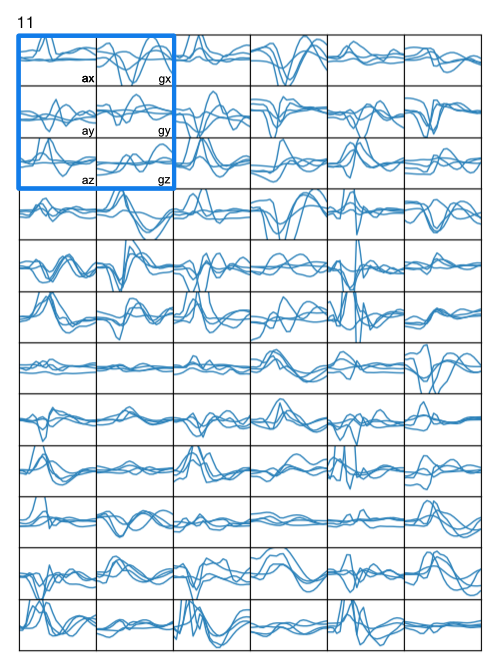
\includegraphics[width=0.8\textwidth]{results/tap4x32.png}
  \caption{The visualization shows the collected gyroscope and accelerometer components for the 4x3 grid. In the top left corner the grid class 11 is shown which corresponds to the top left corner of the mobile device.} \label{fig:taps}
\end{figure}

\subsection*{Input Modality}
\subsubsection*{2x2 grid}
For the comparison between input modalities, we find that for the 2x2 grid, all mean accuracies across devices were higher for index finger tap data compared to classifiers trained with the thumb tap data.

A Wilcoxon signed-rank test shows that the classification results for both input modalities differ significantly. The fold accuracies on thumb data were statistically lower than the fold accuracies on index finger data Z = 27, p < 0.05.

\begin{figure}[h!]
  \centering
  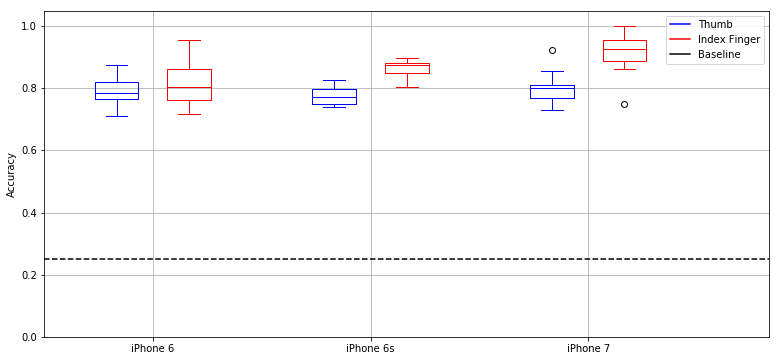
\includegraphics[width=1\textwidth]{results/index-vs-thumb-2x2.png}
  \caption{The figure shows the tap inference accuracies for the 2x2 grid of the 10-fold cross-validation.} \label{fig:participation}
\end{figure}

\begin{table}[h!]
  \centering
\begin{tabular}{|l|l|c|c|c|c|c|}
  \cline{3-6}
  \multicolumn{2}{c}{} & \multicolumn{4}{|c|}{\textbf{Accuracy}}  \\
  \hline
  \textbf{Device} & \textbf{Input Modality} & mean &   min &   max  & std &  \textbf{Classifier} \\
  \hline
	iPhone 6 & Index &      0.82 &     0.72 &     0.95 &     0.07 &  SVM \\
	& Thumb &      0.79 &     0.71 &     0.87 &     0.05 &  SVM \\
	\hline
iPhone 6s & Index &      0.86 &     0.80 &     0.90 &     0.03 &  SVM \\
	& Thumb &      0.78 &     0.74 &     0.83 &     0.03 &  SVM \\
	\hline
	iPhone 7 & Index &      0.91 &     0.75 &     1.00 &     0.07 &  SVM \\
	& Thumb &      0.80 &     0.73 &     0.92 &     0.05 &  SVM \\
	\hline
\end{tabular}
  \caption{Classification results for the 2x2 tapping grid for both input modalities: thumb and index finger.}
\end{table}

\subsubsection*{4x3 grid}
For the 4x3, all mean accuracies across devices were higher for index finger tap data compared to classifiers trained with the thumb tap data. The greatest difference in inference accuracies are to found on the iPhone 7 where 0.7 (+/- 0.08) for index finger records and 0.52(+/- 0.03) for thumb taps.

A Wilcoxon signed-rank test shows that the classification results for both input modalities differ significantly. The fold accuracies on thumb data were statistically lower than the fold accuracies on index finger data Z = 64.0, p < 0.05.


\begin{figure}[h!]
  \centering
  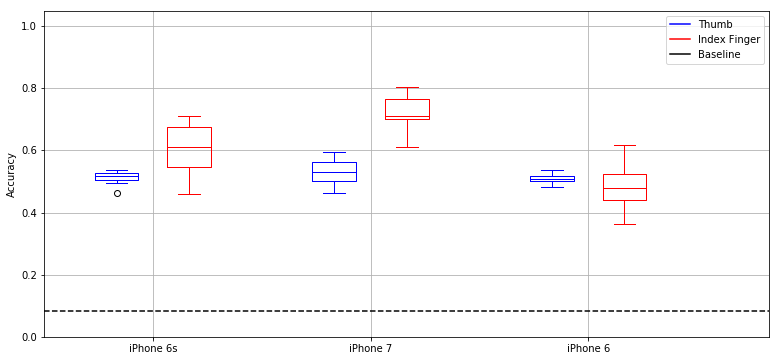
\includegraphics[width=1\textwidth]{results/index-vs-thumb-4x3.png}
  \caption{The figure shows the tap inference accuracies for the 4x3 grid of the 10-fold cross-validation.} \label{fig:participation}
\end{figure}

\begin{table}[h!]
  \centering
\begin{tabular}{|l|l|c|c|c|c|c|}
  \cline{3-6}
  \multicolumn{2}{c}{} & \multicolumn{4}{|c|}{\textbf{Accuracy}}  \\
  \hline
  \textbf{Device} & \textbf{Input Modality} & mean &   min &   max  & std &  \textbf{Classifier} \\
  \hline
	iPhone 6 & Index &      0.48 &     0.40 &     0.56 &     0.06 &  SVM \\
	& Thumb &      0.50 &     0.43 &     0.54 &     0.04 &  SVM \\
	\hline
iPhone 6s & Index &      0.61 &     0.48 &     0.72 &     0.07 &  SVM \\
	& Thumb &      0.47 &     0.43 &     0.51 &     0.03 &  SVM \\
	\hline
	iPhone 7 & Index &      0.70 &     0.56 &     0.80 &     0.08 &  SVM \\
	& Thumb &      0.52 &     0.48 &     0.57 &     0.03 &  SVM \\
	\hline
\end{tabular}
  \caption{Classification results for the 4x3 tapping grid for both input modalities: thumb and index finger.}
\end{table}

\section*{Body Posture}
\subsection*{2x2}
For the 2x2, all mean accuracies across devices were higher for sitting data compared to classifiers trained with the standing data. A Wilcoxon signed-rank test shows that the classification results for both body postures differ significantly. The fold accuracies on standing data were statistically lower than the fold accuracies on sitting data Z = 55.0, p < 0.05.

\begin{figure}[h!]
  \centering
  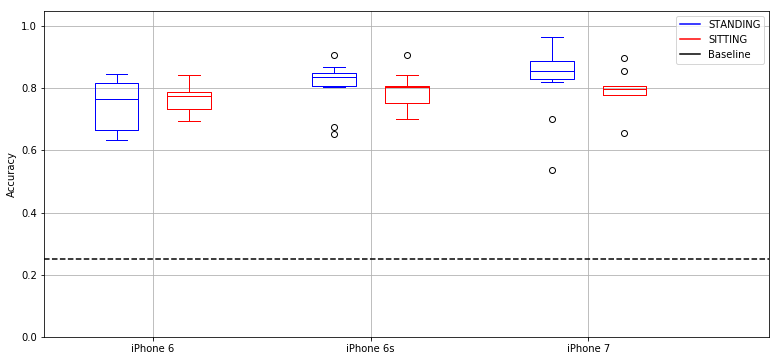
\includegraphics[width=1\textwidth]{results/standing-vs-sitting-2x2.png}
  \caption{The figure shows the tap inference accuracies for the 4x3 grid of the 10-fold cross-validation.} \label{fig:participation}
\end{figure}

\begin{table}[h!]
  \centering
\begin{tabular}{|l|l|c|c|c|c|c|}
  \cline{3-6}
  \multicolumn{2}{c}{} & \multicolumn{4}{|c|}{\textbf{Accuracy}}  \\
  \hline
  \textbf{Device} & \textbf{Input Modality} & mean &   min &   max  & std &  \textbf{Classifier} \\
  \hline
	iPhone 6 & Sitting &  0.84 &     0.68 &     0.97 &     0.08 &  SVM \\
	& Standing &      0.80 &     0.63 &     0.94 &     0.10 &  SVM \\
	\hline
	iPhone 6s & Sitting &      0.87 &     0.72 &     1.00 &     0.09 &  SVM \\
	& Standing &      0.85 &     0.73 &     0.93 &     0.05 &  SVM \\
	\hline
	iPhone 7 & Sitting &      0.95 &     0.88 &     1.00 &     0.04 &  SVM \\
	& Standing &      0.86 &     0.60 &     0.94 &     0.10 &  SVM \\
	\hline
\end{tabular}
  \caption{Classification results for the 2x2 tapping grid for both input modalities: thumb and index finger.}
\end{table}


\subsection*{4x3}
For the 2x2, all mean accuracies across devices were higher for sitting data compared to classifiers trained with the standing data. A Wilcoxon signed-rank test shows that the classification results for both body postures differ significantly. The fold accuracies on standing data were statistically lower than the fold accuracies on sitting data Z = 71.0, p < 0.05.

\begin{figure}[h!]
  \centering
  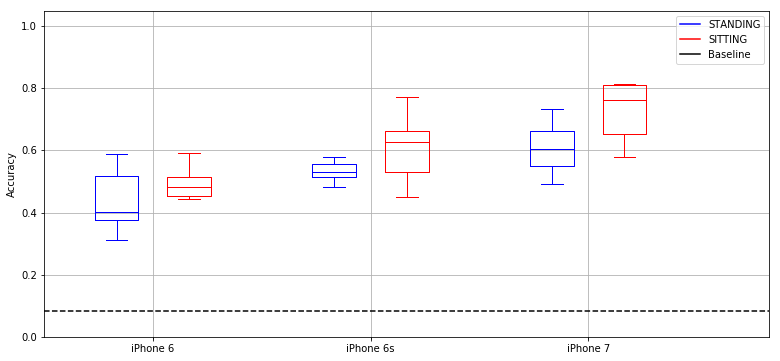
\includegraphics[width=1\textwidth]{results/standing-vs-sitting-4x3.png}
  \caption{The figure shows the tap inference accuracies for the 4x3 grid of the 10-fold cross-validation.} \label{fig:participation}
\end{figure}

\begin{table}[h!]
  \centering
\begin{tabular}{|l|l|c|c|c|c|c|}
  \cline{3-6}
  \multicolumn{2}{c}{} & \multicolumn{4}{|c|}{\textbf{Accuracy}}  \\
  \hline
  \textbf{Device} & \textbf{Input Modality} & mean &   min &   max  & std &  \textbf{Classifier} \\
  \hline
	iPhone 6 &  Sitting &      0.49 &     0.44 &     0.59 &     0.05 &  SVM \\
	{} & Standing &      0.47 &     0.34 &     0.62 &     0.08 &  SVM \\
	\hline
iPhone 7 &   Sitting     &      0.73 &     0.58 &     0.81 &     0.08 &  SVM \\
	& Standing &      0.64 &     0.52 &     0.76 &     0.08 &  SVM \\
	\hline
iPhone 6s & Sitting &      0.61 &     0.45 &     0.77 &     0.11 &  SVM \\
	& Standing &      0.56 &     0.51 &     0.61 &     0.03 &  SVM \\
	\hline
\end{tabular}
  \caption{Classification results for the 4x3 tapping grid for both input modalities: thumb and index finger.}
\end{table}

\newpage {
	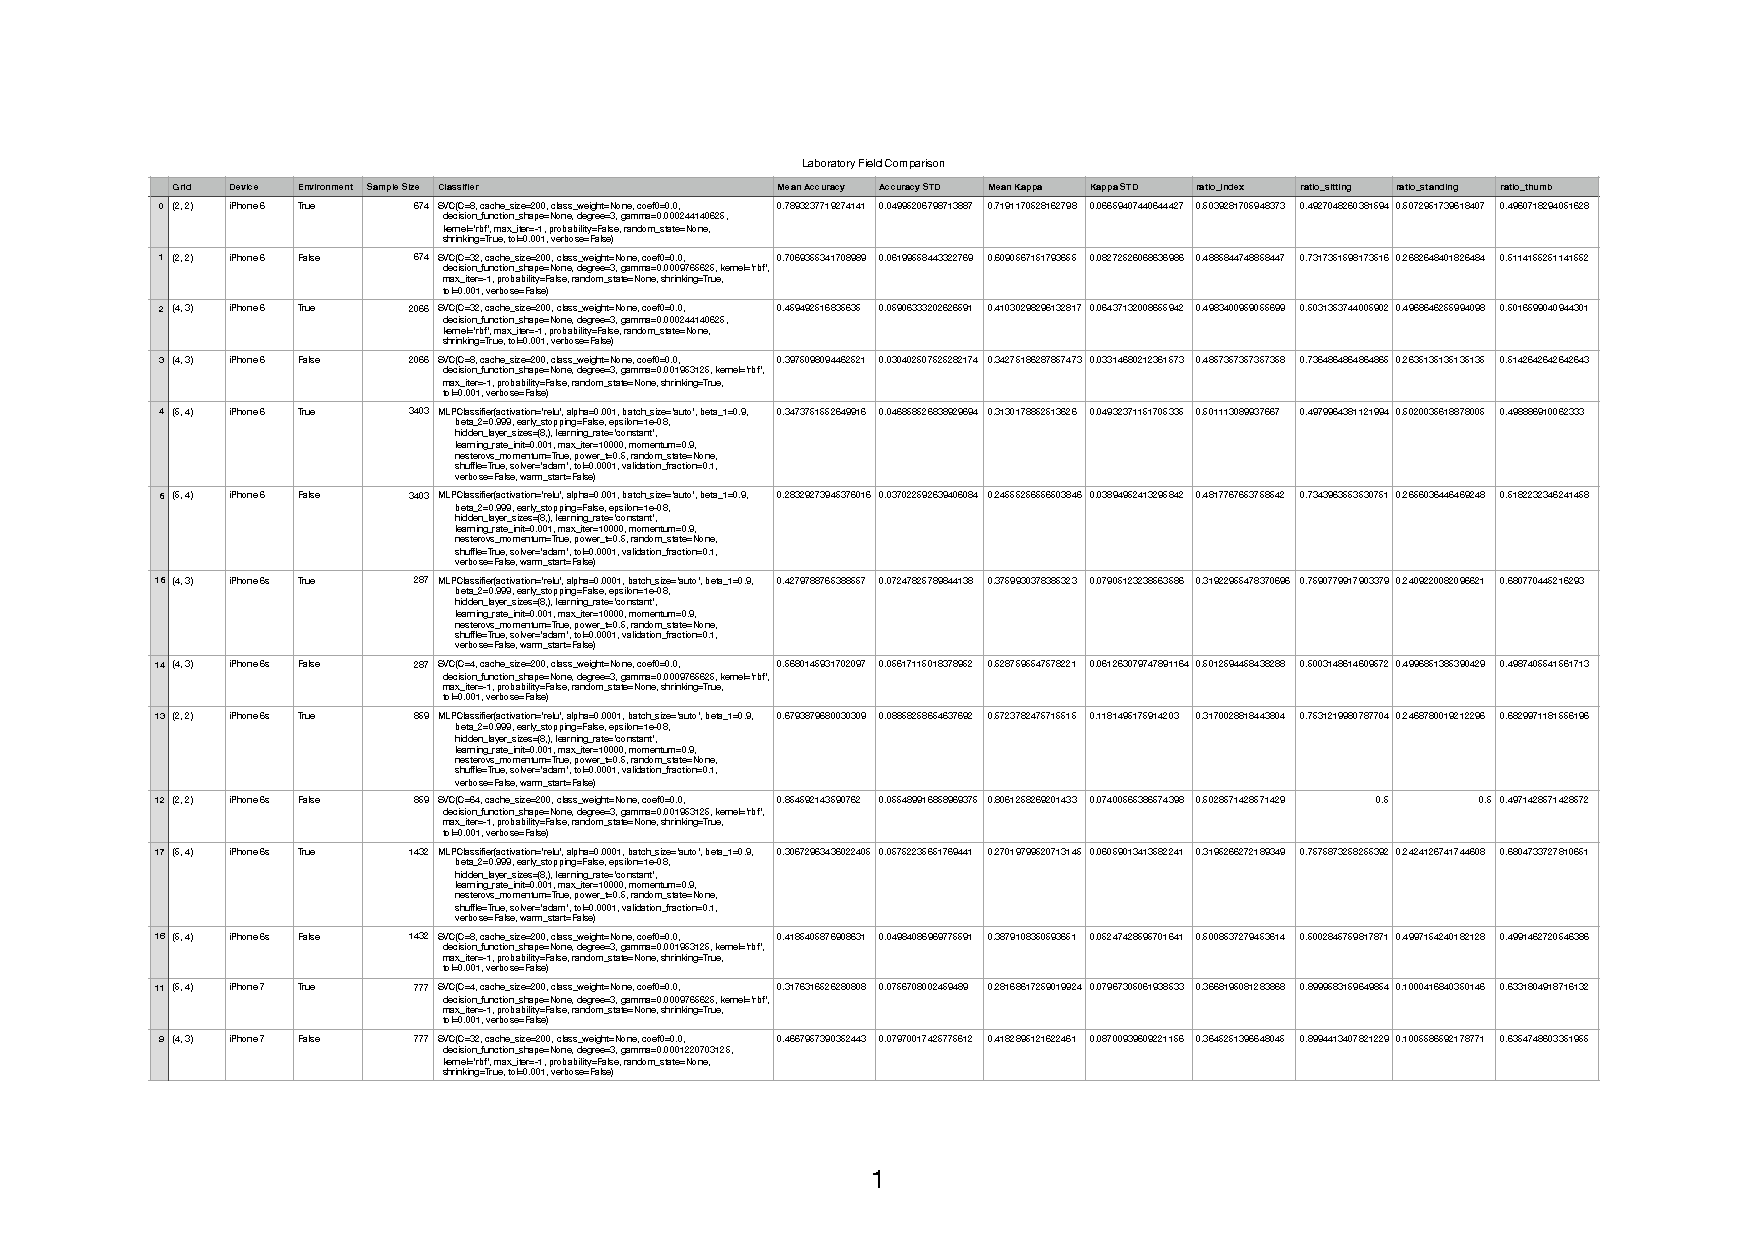
\includepdf[landscape=true, pages=-]{pdf/labfield_print.pdf}
	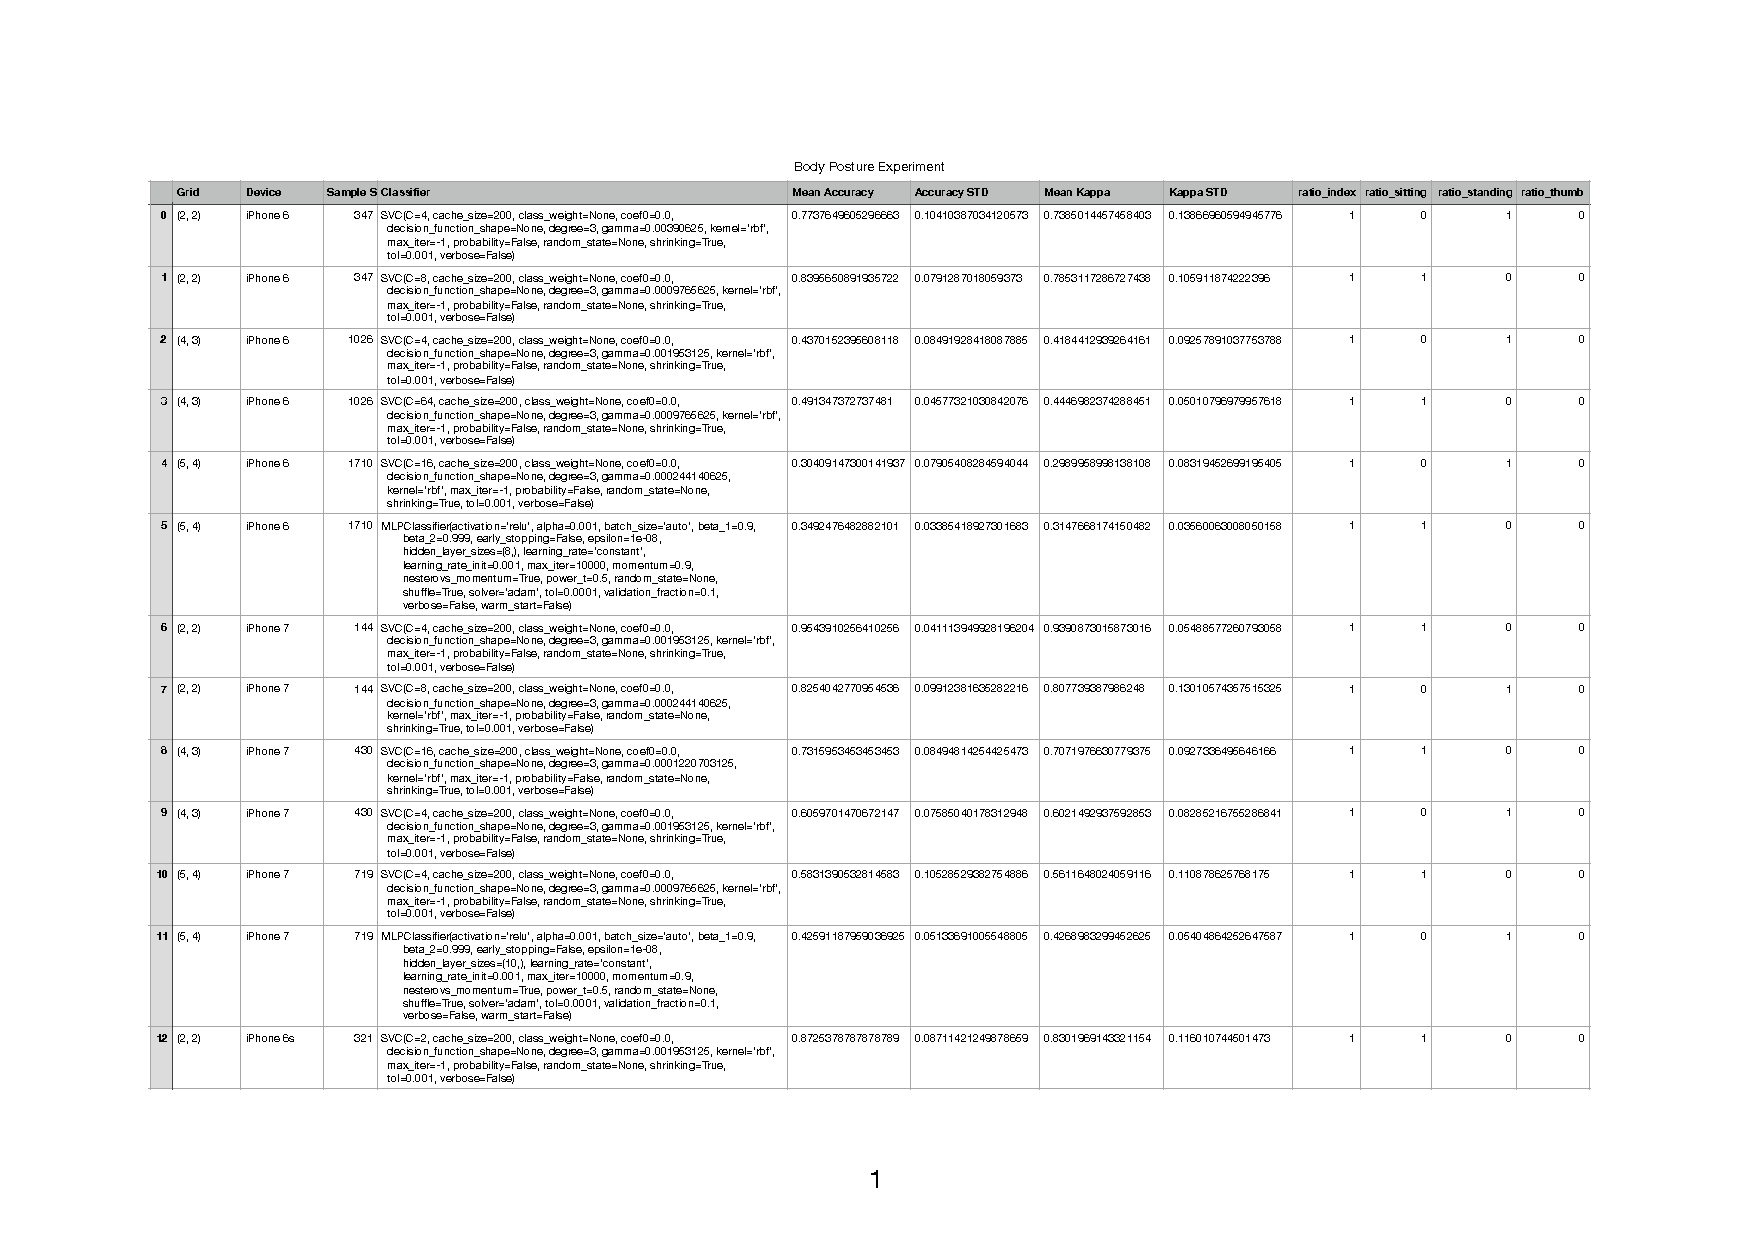
\includepdf[landscape=true, pages=-]{pdf/body_posture_print.pdf}
	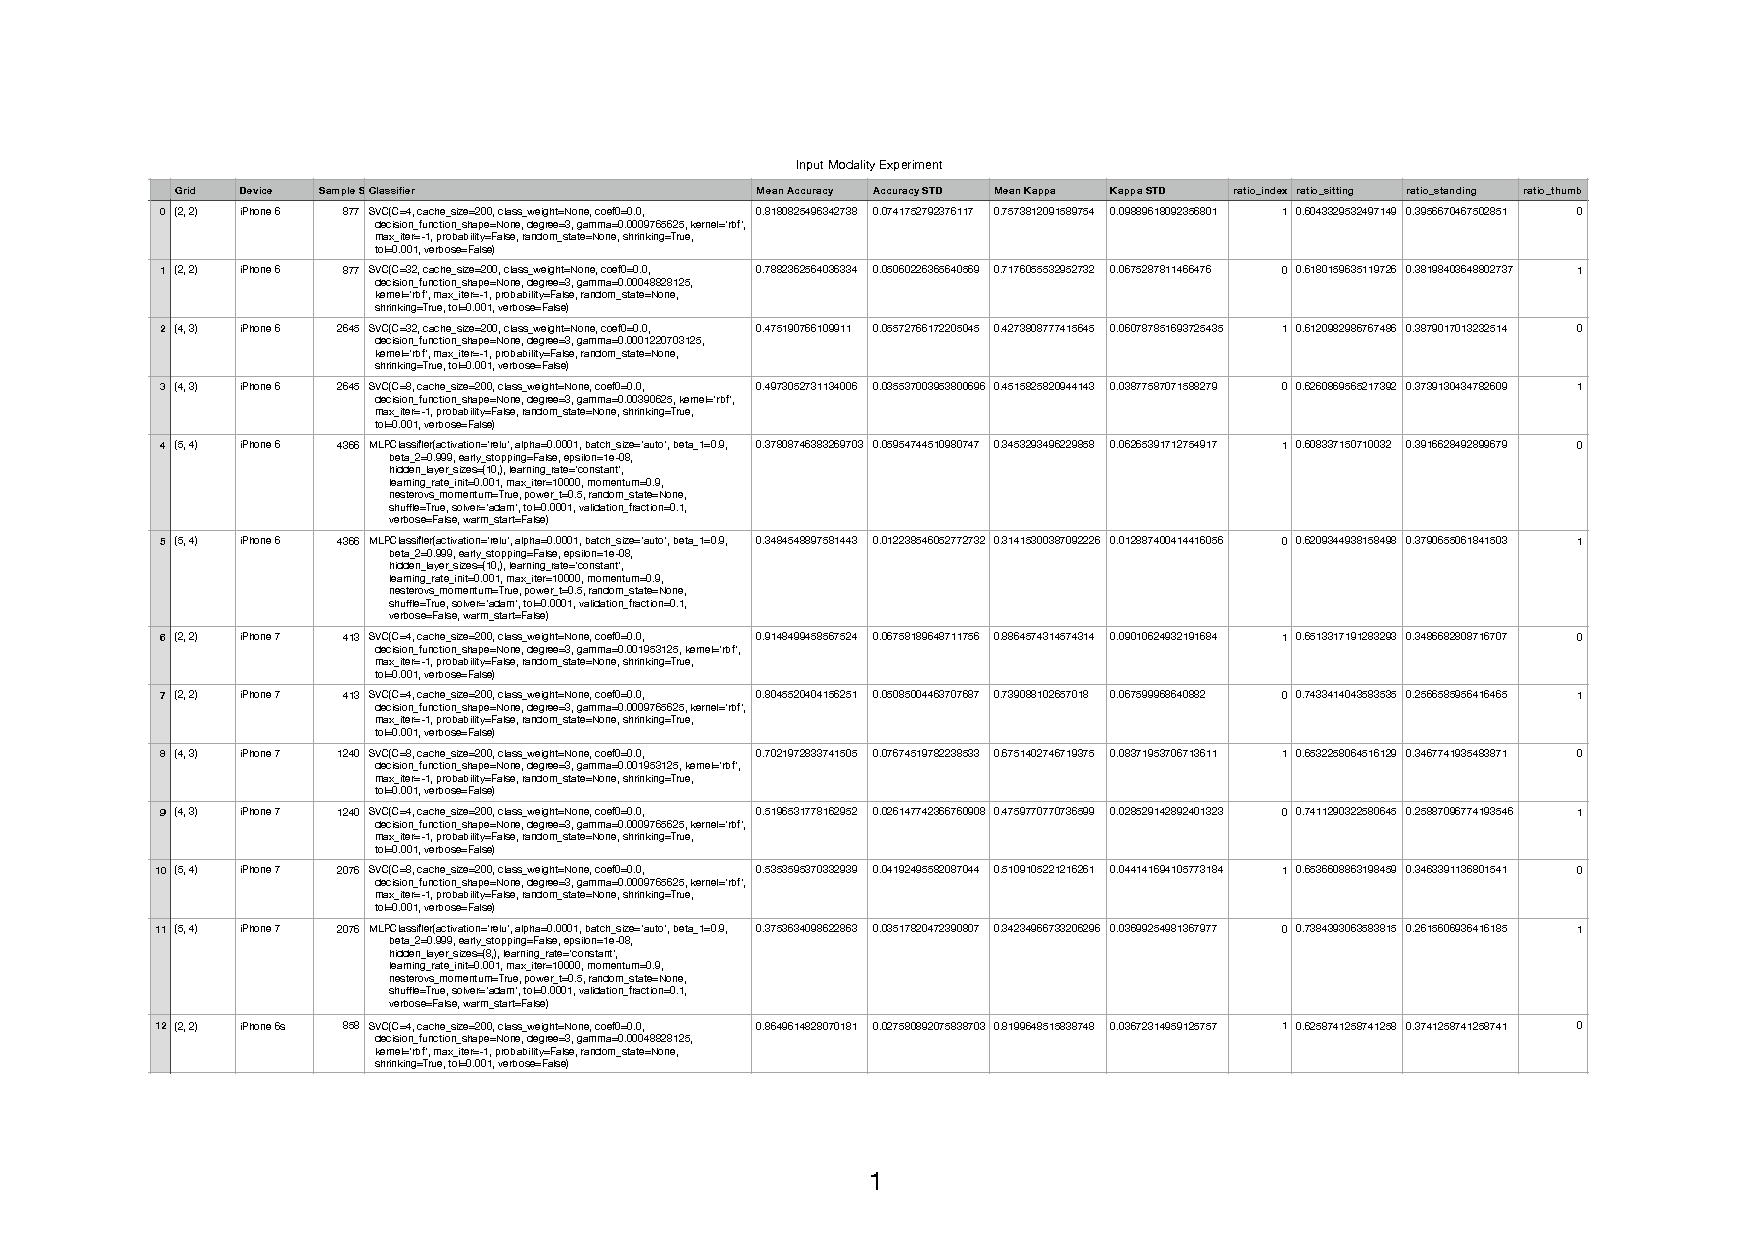
\includepdf[landscape=true, pages=-]{pdf/input_modality_print.pdf}
}


\end{appendix}

\endinput


\end{document}
